\documentclass[12pt,letterpaper]{article}
\usepackage[capposition=top]{floatrow}
\usepackage{epsfig}
\usepackage{amsmath}
\usepackage{amssymb}
\usepackage{setspace}
\usepackage{array}
\usepackage{hyperref}
\usepackage{longtable}
\usepackage{lscape}
\usepackage{pdflscape}
\usepackage{natbib}
\usepackage{ulem}
\usepackage{placeins}
\usepackage[margin=1in]{geometry}
\usepackage{tabularx}
\usepackage[table]{xcolor}
\usepackage{booktabs}
\newcolumntype{Y}{>{\centering\arraybackslash}X}
\usepackage{multirow}
\usepackage{caption}
%\usepackage{subcaption}
\usepackage{tgtermes}
\usepackage[T1]{fontenc}
\fontfamily{qtm}\selectfont
\usepackage{tikz}

\newcommand{\mynoteMM}[1]{\textcolor{red}{[MM note: #1]}}
\newcommand{\SAdded}[1]{\textcolor{red}{#1}}
%\renewcommand{\SAdded}[1]{\textcolor{black}{#1}}
%\renewcommand{\sout}[1]{{}}
%remove comment if don't want notes to show:
%\newcommand{\mynoteMM}[1]{\textcolor{}{}}
%\newcommand{\mynoteSR}[1]{\textcolor{}{}}
\definecolor{azure}{rgb}{0.0, 0.5, 1.0}
\definecolor{gray90}{gray}{.90}
\definecolor{gray80}{gray}{.80}
\definecolor{paleblue}{cmyk}{.2, 0, 0, 0}

\newcommand{\bfbeta}{\ensuremath{\mbox{\boldmath $\beta$}}}
\newcommand{\bfzeta}{\ensuremath{\mbox{\boldmath $\zeta$}}}
\newcommand{\bfgamma}{\ensuremath{\mbox{\boldmath $\gamma$}}}
\newcommand{\bfdelta}{\ensuremath{\mbox{\boldmath $\delta$}}}
\newcommand{\bfomega}{\ensuremath{\mbox{\boldmath $\omega$}}}
\newcommand{\bfc}{\ensuremath{\mbox{\boldmath $c$}}}
\newcommand{\bfx}{\ensuremath{\mbox{\bf x}}}
\newcommand{\bfm}{\ensuremath{\mbox{\bf m}}}
\newcommand{\0}{\ensuremath{\mbox{\boldmath $0$}}}
\newcommand{\defeq}{\mathrel{\mathop:}=}


\begin{document}

\singlespacing

\title{
\vspace{-1.25cm}
Seasonality, Academic Calendar and School \\
Drop-outs in South Asia\thanks{\protect%
The authors are grateful to IFPRI for sharing the data and Ranjana Roy for the data cleaning support. The authors thank the following people for helpful comments (alphabetically): Ariel BenYishay, Austin Davis, Gary Fields, Hyuk H Son, Jessica A. Goldberg, Jonathan Morduch, Kensuke Kubo, Nobuhiko Fuwa, Seema Jayachandran, Takashi Kurosaki, Tomoki Fujii, Yasuyuki Sawada, and participants at ASSA Meeting, NEUDC, Econometric Society Meeting, Hakone Conference as well as seminar series at Hitotsubashi University, GRIPS-FASID, Waseda University, Singapore Management University, National University of Singapore, NanYang Technological University, World Bank, Washington State University, University of Central Florida, Florida International University and IDE. The authors are responsible for the errors. The findings, interpretations, and conclusions expressed in this paper are the author's own, not of their affiliated institutions. \vspace{0.25em}}} 

\author
{\textsc{Seiro Ito}\thanks{
Institute of Developing Economies, IDE-JETRO, 3-2-2 Wakaba, Mihama-Ku, Chiba-shi, Chiba 261-8545, Japan, seiroi@gmail.com.}
{\textsc{ and Abu S. Shonchoy}}\thanks{
Florida International University, Department of Economics, 11200 SW 8th Street, Miami, Florida 33199, USA. Phone: (305) 348-3352,
Email: shonchoy@fiu.edu, parves.shonchoy@gmail.com}}


\maketitle

\vspace{2.5em}
%\vspace{-1.5em}

\begin{abstract}
\vspace{-0.5em}
\singlespacing{
Rural families face tradeoffs in deciding whether to retain their children in school or work in the field. School calendars heighten this tradeoff by not accommodating seasonal agricultural labor demand, leading to dropouts. Utilizing Ramadan school holidays as a natural experiment, we find annual exams overlapping with the harvesting season increase school dropout by 6.6-9.0 percentage points in Bangladesh. Age-specific cohort analysis using national household survey confirms these findings. Exploiting state-level academic calendar variation, we execute complementary analysis with India and find supporting evidence. Our paper suggests careful school calendar design in developing countries by adequately addressing local seasonality.


{\bf Keywords:} Enrollment; child labor; seasonal labor-demand; school calendar; ramadan; drop-out.

{\bf JEL Code:} O13, O15, O38, O53, J23, J24
\vspace{5em}}

%\textcolor{red}{This is Seiro edit.}\\
%\textcolor{blue}{This is Abu-san edit.}

\end{abstract}

\doublespacing

\pagebreak

\normalsize





\section{Introduction}

Local agricultural seasonality is an integral part of rural livelihoods in developing countries, which can seriously affect school continuation for students. Low-income families, who are mostly credit-constrained and often dependent on their children's labor, face a trade-off in deciding whether to retain their children in school or make them work in the field. In agrarian societies, this tension is greatest during the planting and harvesting seasons, when there is a rise in labor demand with escalating wage rates, often leading students to discontinue schooling. Education-related policies in developing countries do not typically address this concern with seasonal work. 

Bangladesh Bureau of Statistics (BBS) estimated that 56\% of all child labor belongs to the agricultural sector in Bangladesh \citep{bbs2003report}. In a detailed education assessment study by USAID, 42\% of rural students are reported to be absent during the harvesting period in Bangladesh, compared to 6.8\% absent during the planting period \citep[][Table IV.D.9, page 110]{Rahman2004}. \SAdded{[In our 2003 data, slightly higher 11-15\% (2.8 to 3.8 days per 25 days) absenteeism is observed.]} This is not a past phenomenon; a recent 2017-18 study on school students in Bangladesh also finds a similar trend in absenteeism among rural children during the time of harvesting \citep{Fujii2019}.\footnote{More recently Primary School Certification Exam (PCSE), which was introduced in 2009, was scheduled in the last week of November in 2010. Unsurprisingly, the Directorate of Primary Education reported a 10$\%$ absenteeism on the first day of this largest nationwide public examination, highlighted in the media \textit{the Daily Star} (click here \url{https://www.thedailystar.net/news-detail-163453}). Interestingly, on the same day, the 24th November 2010, the Daily Star reported bumper production of \textit{Aman} paddy in some parts of Bangladesh (click here \url{https://www.thedailystar.net/news-detail-163434}). } Similarly, high absenteeism is reported in India's rural schools due to such conflict with the agricultural calendar as reported in the paper by \cite{de2016estimating}. Previous studies have investigated the role of technology, weather shocks and price changes in agriculture on schooling; however, the calendar issue (overlapping peak labor demand time with annual grade progression final examination) has not been discussed or documented in the academic literature.

Bangladesh's schooling system follows the English (Gregorian) calendar for academic activities (January-December) and does not accommodate local agricultural cycles. As a consequence of this misalignment, annual examinations in schools, which are typically held at the end of the calendar year (December), coincide with the peak harvest period of the major wet season paddy called \textit{Aman}.\footnote{\textit{Aman} rice is the largest crop in Bangladesh by area and the second-largest by cereal production.} During the harvesting period, student's schooling is routinely interrupted by the active involvement in rice production and post-production processes. Advancement to the next higher grade typically depends on achieving satisfactory scores in the final exam \citep{ADB2017}. When the harvesting period overlaps with the final examination period, it can result in attaining lower academic scores or missing exams altogether. This prompts some student to discontinue or drop out of school. 

Poor agricultural households, who typically cultivate small-hold-tenure land, are generally unable to hire external labor because of labor market imperfections, such as shortage of labor at the harvesting time \citep{rosenzweig1988labor}, liquidity constraints raising the shadow price of labor input owing to cash payment requirements \citep{singh1986agricultural}, and imperfect substitution between hired and family labor \citep{de1991peasant}.\footnote{Even if farmers are not constrained, parents may want their children to learn essential farming skills by actively engaging in the harvesting process \citep{bhalotra2003child}, or illiterate farmers are myopic to realize the importance of children's human capital formation or return to education \citep{BalandRobinson2000}. } Moreover, the opportunity cost of schooling increases during peak labor demand time as the marginal revenue product of child labor increases. The seasonal variations in opportunity costs of schooling has not attracted due attention in both policies and academic literature. 

To address this gap, we estimate the impact of increased seasonal labor demand during the annual final exam on school continuation. Exploiting the shifting Ramadan dates by years that force the high stake final exams to be held either in or off the haversting period, which we consider as exogenous, we compare schooling outcomes of the year that exams ovelap with the harvest with the year that does not. We find that the overlap contributes to school dropout for students from agricultural households compared to non-agricultural households. 

During 1999-2001, owing to the mandatory school holidays in \textit{Ramadan}, schools have brought forward their examination schedule to the pre-harvest season in Bangladesh, a time of reduced local agricultural labor demand. Using student-level panel data from 1999 and 2002 and employing a difference-in-differences (DID) estimator, we compare school enrollment between children from agricultural and non-agricultural households to assess the differential impacts of seasonal labor demand changes on school continuation. 

We find that annual exams overlapping with the \textit{Aman} harvesting period decrease school continuation (increase dropout) for children from agricultural households by 6.6 to 9.0 percentage points (compared with a 35\% dropout between 1999-2002 by non-agricultural households). We document that this impact is primarily coming from the boys enrolled in secondary school, suggesting the brawn-based interpretation that boys who are more productive in agricultural activities tend to get pulled out of schools \citep{PittRosenzweigHassan2010}. 

To test the common trend assumption necessary for the consistency of the DID estimator, we show that it is likely to hold using three data sources: One with a later round of the primary sample and the other two with nationally representative household sample surveys of Bangladesh. \SAdded{The common trend tests using India data also shows ... (need to add here)}

To rule out possible confounders, we use placebo tests and a series of robustness checks. The placebo test, where we use the later rounds of data under which the exam schedule always coincides with the harvest, finds no effects on the same cohorts in later rounds and on the younger cohorts of the same age observed in the later round. Most importantly, the boys subsample show no effects in all placebo tests. We also compare our estimates with Muslim and non-Muslim households to disentangle any confounding factors, such as festivity and fasting, and flood-affected and unaffected areas to see if a natural disaster-driven shock is driving the results. We find that these factors have statistically nil impacts. In further assessing the impact mechanism, we find higher absenteeism during the agricultural season among the agricultural households. This suggests absence is one of the plausible factors driving these estimates. In addition to higher dropout rates, we also find that the grade progression is slower for children of agricultural households even when they stay on school. This indicates that the opportunity costs of human capital are higher for the agricultural households when academic calendar is not adjusted for local agricultural seasonality. 

To check the validity of this finding, we examine the overall impact of \textit{Ramadan} induced temporary changes in the academic calendar on educational outcomes in Bangladesh. Using the latest round of the nationally-representative Household Income and Expenditure Survey (HIES 2016), we conduct an age-specific cohort analysis of academic outcomes in rural areas. Our analysis suggests that the school-going age cohort in 1999 significantly benefited from this favorable academic calendar, which reduced the urban-rural education gap by 0.46 years and increased the probability of completing primary, secondary, and higher secondary schools by 5.3, 5.3, and 3.3 percentage points, respectively. Using a Mincerian regression, we find this impact generates approximately a three percent economic return (measured with annual wage earnings) for the beneficiary cohort owing to a favorable academic calendar.

In an effort to assess the external validity of findings, we also used data from India to exploit the state-level academic calendar variations against primary crop harvest seasons. Unlike Bangladesh, where a national homogeneous school calendar is utilized, in India, this conflict occurs due to the variation in the state-level school calendar and local primary crop harvesting season, making some states' academic routines unfavorable for students from agrarian families. It shows similar negative impacts (5.34 to 6.55 percentage points reduction) of academic calendar mismatch on school continuation for agricultural household children, consistent with our findings in Bangladesh. This further indicates that our finding may be applicable in South Asia with relevant populations (dominant agricultural sector, credit-constrained, and poor smallholder farmers). 

When we take our findings as the inadequacy of addressing local agricultural seasonality in education policy, they may have broader implications that are not limited to Bangladesh or India. In Africa, the temporary withdrawal of children from school during harvesting and times of hungry-season-led migration results in permanent withdrawal from schools \citep{ andvig1999child, Colclough2000, Hadley2010, kadzamira2003can, WorldBank1998}.\footnote{In Ethiopia, school enrollment begins in September; however, children leave schools in November due to the harvesting labor demand of \textit{meher} season crops, which are Barley, Maize, Wheat, Sorghum, Oats, and Millet. In Kenya, a similar problem occurs, as maize harvesting (October-November) overlaps with the Kenyan Certificate of Secondary Exam (KCSE) in November. We observe such conflict in school schedules and seasonality in other countries such as Malawi, Nigeria, and Nepal. } The agricultural seasonality is a difficult issue when a uniform school calendar is implemented in multiple climatic zones. Countries such as Tanzania, Brazil, Colombia, and India have multiple climatic zones suitable for different crops. Strictly enforcing a country-wide uniform academic calendar in such countries may conflict with local agricultural seasonality, which can adversely affect the schooling of children of agricultural households. 

Our study contributes to the literature by identifying the demand-side constraints on schooling in developing countries. Research on the demand-side aspects of schooling suggests that the opportunity cost of schooling can be exorbitantly high for children from economically marginalized households. This is due to liquidity constraints  \citep{JacobySkoufias1997, BeegleDehejiaGatti2006}, the inability to insure against shocks to income-earning activities \citep{Jensen2000, deJanvryetal2006, Case2006}, comparative advantages in remunerative physical work \citep{PittRosenzweigHassan2010}, and children's inability to become decision-makers for their human capital investments \citep{BalandRobinson2000}. The existing literature documents a higher opportunity cost of schooling through positive rainfall shocks that increase agricultural productivity in India \citep{shah2017drought}, new manufacturing factory openings \citep{atkin2016endogenous} and gold mining \citep{santos2018blessing}. Our study highlights another important opportunity cost issue caused by a mismatch between the academic calendar and peak seasonal agricultural labor demand.

This study also speaks to the literature on the effects of academic calendar reforms, such as all-year schooling \citep{ mcmullen2012impact, graves2010academic}; shorter school week \citep{anderson2015does}; early school starting hours \citep{cortes2012role,  hinrichs2011bell, edwards2012early, carrell2011s}; and reduction in compulsory years of schooling \citep{elsayed2021less}. Two papers closest to our setting study Malawi; \cite{allen2024double} documenting adverse school progression due to greater overlap of school and farming calendar and \cite{dillon2021selling} showing mixed evidence on schooling improvement when the government aligns academic session starting time with harvesting to facilitate school fee payments for credit-constrained farmers. Lastly, our study strengthens the literature on the impact of child labor on schooling that documents the concurrence of work and schooling \citep{RavallionWodon2000, Edmonds2007, Dumas2012}; and negative correlations between exam scores and work hours \citep{AkabayashiPsacharopoulos1999, Heady2003, Gunnarsson2006}.


\section{Context and Identification\label{sec.id}}
\subsection{School Education and Academic Calendar in Bangladesh}

Bangladesh's educational system comprises Primary (grades 1-5, ages 6-10), Secondary (grades 6-10, ages 11-15), and Higher Secondary (grades 11-12, ages 16-17) schooling followed by tertiary and vocational education \citep{kono2018primary}. Schooling is compulsory up to grade 8. However, it is not enforced. 

The academic year in Bangladesh runs from January to December. Since its independence, Bangladesh's school learning assessment system has mostly followed two pen-and-paper-based exams conducted by schools annually, known as half-yearly (mid-year, conducted in June) and final (year-end, conducted from late November to mid-December) exams. These assessments are prepared and graded by teachers of the respective schools. The mid-year exam is somewhat formative, while the year-end exam is considered the final evaluation. Students are promoted to the next higher grade based on their performance in the annual exam. End-of-year exams are binding for all grades, and not passing the exam would prohibit grade progression \citep{de2004school,begum2008school,ADB2017}. Figure \ref{school_calander_2019} in Appendix A4 presents a typical Ministry of Education (MoE) provided academic calendar that clearly shows the half-yearly and final exam timing for Bangladesh and these dates are fixed at the beginning of the academic year (\cite{ADB2017}, page 73).\footnote{The Bangladesh National Education Commission has recommended the addition of three exams - first-term, second-term, and third-term, which were introduced later, with the third term acting as the annual exam. However, currently, primary schools continue with the annual three-examination system, while the Ministry of Education (MOE) has recently switched secondary schools to a two-examination system (half-yearly and annual). These two exams have already been scheduled, and all schools adhere to this new system. } 


\subsection{Rice Harvesting, Agricultural Calendar and Child Labor \label{sec.rice}}

Rice is the principal agricultural product in Bangladesh, accounting for 74\% of the gross crop area \citep{tisdell2019agricultural}. Out of three cropping seasons (Boro, Aus, and Aman) of rice production \citep{laborte2017riceatlas}, \textit{Aman} is the largest in terms of the amount of area utilized, as mentioned in footnote 1. \textit{Aman} is a traditional rain-fed paddy variety planted in July-August and harvested from late November to mid-December \citep{shelley2016rice}.\footnote{The agricultural calendar is not static, and it may shift by a week or so due to climatic conditions of the year. } \textit{Aman} intensity varies across regions; however, given the dominance of rice and the lack of agricultural diversity, other crops in any season are very limited, capturing only 2.67 and 1.97\% of the gross cropped area in Bangladesh \citep{tisdell2019agricultural}. It is well documented that agricultural wage fluctuates seasonally, peaking during harvesting (and sometimes during planting). Figure \ref{wage} taken from \citet{rahman1988labour} portrays wage variation for agricultural wage laborers across the seasons, with wages peaking during the \textit{Boro} and \textit{Aman} paddy harvesting seasons in April-June and November-December, respectively.

\begin{figure}[h!]
\centering
\includegraphics[width = 17cm, height = 13cm]{Figures/Seasonal Agri Wage.jpg}\\
\caption{Seasonal variation in agricultural wage in Bangladesh}
\label{wage}
\end{figure}

These hikes in agricultural wages during harvesting are driven by the rapid rise in local labor demand within a short period of time owing to time-sensitive harvesting (hence, not allowing spatial labor movement) coupled with liquidation demand to pay the bills accumulated throughout the year \citep{burke2019sell}. Moreover, the lack of credit access makes it difficult for marginalized farmers to pay for hired labor, forcing them to depend on family labor. According to the \cite{bbs2003report} National Child Labor survey 2002-2003, approximately 7.4 million children in Bangladesh are engaged in child labor, of which 23.5\% are in paid work and another 57\% are in unpaid family work. Agriculture remains the dominant sector for child labor, as reported in the later round of the child labor survey \cite{bbs2013report}. The age distribution of child labor overwhelmingly belongs to the 10-18 age category, comprising 96\% of all child labor in Bangladesh.

Children engaged in rice production need to engage in the planting, harvesting, and its subsequent tasks, which include threshing, husking, storage, transportation, and selling the harvested goods in the market \citep{chowdhury2009participatory}. Children who participate in harvesting are also get exposed to higher risks of injury due to the utilization of traditional tools (like sickles). Additionally, the physically demanding nature of harvesting work, combined with work-related fatigue and lacking academic support at home (especially for first-generation learners), further hinders academic preparation for year-end exams and progression.\footnote{In addition, several landless families depend on seasonal agricultural work opportunities. The adults of these families, predominantly male, work extensively during the harvesting period, which requires frequent migration out of the village, while children in the household take care of the livestock and other activities (like fetching water and hay-stacking for fodder). } Technically, a student can repeat the grade due to unsatisfactory performance in the yearly final exam. However, grade repetition is not encouraged and very few do so\footnote{The percentage of repeaters in Primary education is only 4\% and 1\% for Bangladesh and India, respectively. \url{https://data.worldbank.org/indicator/SE.PRM.REPT.ZS} }; as a result, failing a grade typically leads to school discontinuation.


\subsection{Ramadan timing as an identification strategy}

Bangladesh is predominantly a Muslim country, and \textit{Ramadan} is a compulsory activity for Muslims. During \textit{Ramadan}, schools are instructed by the Ministry of Education to declare holidays to accommodate and encourage religious practices for children. However, the schedule of these holidays is not fixed, as the Islamic months follow the lunar calendar system. Therefore, \textit{Ramadan} drifts 11-12 days per year on the solar calendar.

From 1999 to 2001, \textit{Ramadan} was observed in December. Consequently, schools had to move their annual final examinations by one month earlier to November, the off-harvest season for \textit{Aman} rice, to accommodate the completion of the academic schedule and holidays. This created only a small overlap between the peak seasonal labor demand period for \textit{Aman} rice and the final examination period. Three years later, in 2002, owing to shifts in lunar calendar dates to the Gregorian calendar, \textit{Ramadan} was celebrated in November. Schools declared holidays in that month and scheduled final examinations in December, which is the usual schedule that overlapped with the \textit{Aman} harvest season. 


\begin{figure}[bt]
\centering
\includegraphics[width = 10cm, height = 9.5cm]{Figures/Framework.jpg}\\
\caption{Sequence of Events.\protect\footnotemark}
\label{schedule}
\end{figure}

\footnotetext{Timing of the annual final exams, \textit{Ramadan}, and the peak harvest period for \textit{Aman} rice. \textit{Ramadan} shifts by approximately 11-12 days each year. The starting dates of \textit{Ramadan} in the different years are as follows: December 9, 1999; November 27, 2000; November 16, 2001; November 6, 2002; and October 27, 2003. The years in shaded rows indicate the years compared in this study using a natural experimental framework. This is a simplified schematic representation; the peak harvest season may shift by year and region. }

\textsc{\small Figure \ref{schedule}} depicts the schematic explanation of the timing of these events. In 1999, the annual final examination period partially overlapped with the harvest period. In 2002, the examination and harvest occurred concurrently after the \textit{Ramadan} holidays. For students preparing for the examinations, this implies that they faced a lower marginal product of labor or smaller seasonal labor demand during the examination period in 1999-2001 than during 2002. We consider this variation in seasonal labor demand during the examination period as a natural experiment that generates a productivity shock, as can be expressed in a simple two-period model (Appendix \ref{app_a1}).

We primarily use the longitudinal data of 1999, 2002 (collected in subsequent planting season of 2000, 2003, respectively) to estimate the impact of peak seasonal labor demand during the examination period --- a variation created by \textit{Ramadan} school vacation --- on the school continuation in Bangladesh. To separately indentify the impacts from time effects, we compare the agricultural and non-agricultural households. Our identification strategy is similar to that used by \citet{OosterbeekKlaauw2013}; taking the time difference of the same individual to eliminate individual fixed effects while using differences in exposure to harvest labor demand between households during exam periods to identify its impacts on school continuation.\footnote{The \textit{Ramadan} timing variation as a natural experiment has been successfully applied in the economics literature. \citet{AlmondMazumder2011} employ \textit{Ramadan} as a natural experiment for forcing smaller food intake. They control for its seasonality by exploiting the shifting nature of \textit{Ramadan} that results from its determination according to the lunar calendar. \citet{OosterbeekKlaauw2013} exploit the same shifting pattern of \textit{Ramadan} over a five-year period as a source of differing exposure to fasting and estimate its impacts on the examination scores of Muslim graduate students in the Netherlands. \citet{Campante2013} examine the impacts of \textit{Ramadan} fasting on the labor market and economy-wide outcomes. }

\subsection{Identification challenges \label{sec.identification_challange}}

The challenges we face with this identification strategy are threefold. First, there is no natural control group, as school holidays given during \textit{Ramadan} are nationwide phenomenon. Therefore, we compare children from agricultural households as the ``treated'' who face higher exposure to seasonal agricultural labor demand, with non-agricultural household children as the ``control.'' This is based on the assumption that poor agricultural families typically engage their children in farming activities during the harvest season to reduce the cost of harvesting and reap the benefits of greater seasonal labor demand and a higher marginal product of labor. In addition to these labor supply-side justifications, one can consider the demand-side preference for children from agricultural households because they have stronger ties with the agricultural community, more seasonal agricultural-based job networks, and more experience in agriculture activities, all of which make them more employable.\footnote{We also note that non-agricultural households tend to face peak labor demand, if any, at different times of the year, rather than during the harvest season (e.g., during new year celebrations). }

Second, empirical supports for the common trend assumption are necessary for the consistency of estimates. Owing to data limitations, we compare the enrollment changes between the treatment and control groups with later waves of the main data source using the 2002 and 2006 survey rounds. We also test the common trend assumption using the latest round of the National Representative HIES of Bangladesh by comparing various birth cohorts of rural and urban areas, which we proxy as agricultural and non-agricultural households.  All these empirical exercises support that the common trend assumption is satisfied.  
 
Third, because we utilize a natural experiment that lacks fine control of events, there may be other possible confounding factors that have affected only agricultural households in the observed years. For instance, in 1999, the annual final examinations were conducted before the harvest and the \textit{Ramadan} school holidays. In 2002, the examinations were scheduled during the harvest and after \textit{Ramadan} school holidays. Therefore, in our natural experiment framework, there exist two potential ``treatments,'' which are: a) Examination coinciding with vs. avoiding the harvest season, and b) Examination before vs. after the \textit{Ramadan} school holidays. Throughout our analysis, we emphasize the effect of point (a) by comparing the impact of the examination calendar shift on agricultural and non-agricultural households. For point (b), we assume that conducting examinations before or after school holidays similarly affects students in agricultural and non-agricultural households. In 2002, annual exams were conducted after a school break, which could have impacted school continuation (for example, students had adequate opportunities for proper rest, which might have improved academic continuation). However, this is true for students from both agricultural and non-agricultural households. We assume that there is no particular reason why having a school break before the exam systematically affects students only from agricultural households to discontinue schooling. We test this assumption using the HIES 2016, employing older cohorts for whom \textit{Ramadan} holidays occurred after the harvest and final exam season. Our estimates indicate no systematic difference in having long holidays before the exam. 

In addition to checking the possible advantages of having a holiday before the exam, we also examine the possible disadvantages of having festivity-related holidays that may affect subsequent exam performance. For instance, the home-learning environment during the festival period may differ between agricultural and non-agricultural households, which can systematically affect exam preparation and school continuation. To verify this empirically, we compare Muslim and non-Muslim households in the main sample. Since non-Muslims do not fast and are less prone to be affected by festivities, this exercise helps us disentangle the festivity impact, which is statistically negligible, and our primary findings remain unchanged. This also checks the impact of fasting; non-Muslim students do not fast; therefore, the statistically zero estimates for non-Muslims affirm that fasting is not the source of enrollment rate variations between households. 

Finally, one could show concern that natural disaster-related shocks (such as floods) could negatively affected the schooling of agricultural households in 2002. This can systematically drive children of agricultural households out of schools. To check this possibility, we test the impacts of floods by using a dummy variable of flooded areas at thana (sub-district) level. We find no evidence that floods disproportionately affected the children of agricultural households. More on the robustness checks are given in Section \ref{sec_DID}. 

\section{Data} 
\subsection{Definitions and descriptive statistics}

The main data-set we use is a panel data set collected in 2000, 2003, and 2007 in rural Bangladesh by the International Food Policy Research Institute (IFPRI). It surveyed 600 households from 60 villages in 30 unions (sub-sub-districts) of 10 thanas (sub-districts) to investigate the impacts of Food for Education (FFE) programs on school enrollment. The sample was selected using the following protocol: Ten thanas were first randomly selected with probability proportional to size (PPS) based on thana-level population data from the 1991 census, and two FFE unions and one non-FFE union were selected per thana.\footnote{This indicates that the choice of unions is not random. So the sample cannot be regarded as a representation of overall rural Bangladesh. However, we consider that it gives reasonable representative information about rural and economically disadvantaged areas of the country. } From each union, two villages were randomly selected with the PPS using village-level population data from the 1991 census. A complete census of the households was then conducted in each of the selected villages, and ten households that had at least one school-age child were randomly selected in each village from the census list of households. Two thanas were dropped from the 2002 survey by the IFPRI, making the panel data include eight thanas. In total, 3,326 individuals were surveyed. 

The survey was conducted in three rounds in September-October 2000, 2003, and 2007. These survey rounds captured enrollment information after completing the school examinations in the 1999, 2002, and 2006 academic years. Given the enrollment information captured through survey timing, we refer to enrollment information as "school continuation to 2000" and "school continuation to 2003."

In our main DID analysis, we use the balanced portion of the 1999-2002 survey data with an age cut-off of 10-18 years old in 1999, consisting of 626 individual observations. Our sample is built on parent(s)-child tuples (nuclear households) to control for parental characteristics, excluding 56 of the 682 individuals who do not have information about their parents. We set the lower age cutoff at ten years old, based on the definition of child labor used in the Labor Force Survey (LFS) of Bangladesh, capturing both primary and secondary school-enrolled students.\footnote{Compulsory school enrollment for primary education in Bangladesh is from age 6-10. For more information, see \url{http://uis.unesco.org/en/country/bd.} } We also use different age cutoffs (11-18 and 12-18 years) for robustness checks. Our main results remain qualitatively unchanged if we retain dropped individuals,\footnote{Not reported but available upon request.} or if we use different lower-age cutoffs. We also examined if there is any indication of non-random attrition and found no statistical evidence (reported in Table \ref{tab attrition comparison} and discussed in Appendix \ref{app_a3}).

For placebo regressions and testing common trends, we use the balanced portion of the 2002-2006 data. When we use the same individuals of the main estimation who were 10-18 in 1999 (1999 cohort), the placebo sample size becomes 616. When we use individuals aged 10-18 in 2002 (2002 cohort), the placebo sample becomes 812. A detailed description of the data cleaning, selection process, and descriptive statistics of the variables used in the main and placebo estimation are available in Appendix A3.\footnote{The 1999 and 2002 data sets are known as the \textit{Impact Evaluation of Food for Education Program in Bangladesh 2000}, and \textit{Comparing Food versus Cash for Education program in Bangladesh 2003} data set, respectively. The 2016 round data set is known as \textit{Chronic poverty and long-term impact study in Bangladesh}. For more information, see \url{https://www.ifpri.org/publication/impact-evaluation-food-education-program-bangladesh-2000}, \url{https://www.ifpri.org/publication/comparing-food-versus-cash-education-program-bangladesh-2003}, and \url{https://www.ifpri.org/publication/chronic-poverty-and-long-term-impact-study-bangladesh.} }

In our main DID analysis, we compare the enrollment information of agricultural and non-agricultural households in 1999 and 2002.\footnote{Here, enrollment information confirms the school continuation of each student as the discontinued student does not enroll in school at the beginning of the academic year. Schools typically confirm this by the middle of the academic year in Bangladesh, when they are obligated to report this to the local administration and the education ministry. } To define an agricultural household, we use the income source information and treat the household as agricultural if the primary income source is farming or agricultural labor. For robustness, we also consider a range of definitions that regard a household as agricultural if any household member reports his or her occupation as agriculture or if a household cultivates agricultural plots. The different definitions are highly correlated, and the estimated results are similar under any definition, as reported in Appendix \ref{app_a4}.\footnote{We found that 9.7\% of reported ``occupation as agriculture'' is associated with non-agricultural work as its primary income source. Accordingly, our default definition of agricultural household, which is a union of occupation and income-based definitions, gives smaller impact estimates than income source or head's reply-based definitions. }


\begin{table}
\begin{minipage}[t]{.7\paperwidth}
\hfil\textsc{\normalsize Table \refstepcounter{table}\thetable: \begin{minipage}[t]{.6\paperwidth}
Summary Statistics and Contrasts of agricultural and non-agricultural Households \\ 
\end{minipage}\label{ag vs nonag}}\\
\setlength{\tabcolsep}{1pt}
\renewcommand{\arraystretch}{.75}
\hfil\input{Tables/AgNonAgDestat.tex}\\
\renewcommand{\arraystretch}{.9}
\setlength{\tabcolsep}{7pt}
\hfil\begin{tabular}{
>{\hfill\scriptsize}p{1cm}<{}
>{\hfill\scriptsize}p{.25cm}<{}
>{\scriptsize}p{.6\paperwidth}<{\hfill}}
Source:& \multicolumn{2}{l}{\scriptsize Compiled from IFPRI data. All information is from 1999.}\\[-1ex]
Notes: & 1. & Columns: For each variable, the top rows indicate the mean and $p$ values. The bottom rows indicate the standard errors of the means. Standard errors are clustered at the thana level, and the Satterthwaite correction for degrees of freedom is applied to account for the small number of clusters. Agricultural households are defined by household income source includes agricultural activities (farming, agricultural labor). The column headed by $t$ indicates $p$ values of zero difference using standard t-tests. The column headed by Satterthwaite implies $p$ values of zero difference with cluster-robust standard errors and Satterthwaite corrections.\setlength{\baselineskip}{8pt}\\[-1ex]
& 2. & Rows: Enrolled status is an indicator variable for school enrollment. Head primary, Head secondary, Spouse primary, and Spouse secondary are the indicator variables for highest educational attainment. The number of older brothers/sisters is the number of older siblings per child. Per-member landholding is the per-member landholding of the household in decimals. The per-member non-land assets are the per-member non-land asset values in 1000 Takas. Piped water and structured toilets are indicator variables for household ownership of each facility. ``Non-Muslim'' is an indicator variable for households with heads who do not identify themselves as Muslim. 
\setlength{\baselineskip}{8pt}
\end{tabular}
\end{minipage}
\end{table}

Given that agricultural and non-agricultural households engage in different types of economic activities, we expect their characteristics to differ. We compare and test for differences between them, as presented in \textsc{\small Table \ref{ag vs nonag}}. One can note a few differences: Only a few spouses of agricultural household heads are likely to have education up to a secondary level. Agricultural households have more land holding per member, which is unsurprising as their main income generating activity is farming. There are more female-headed households among non-agricultural households who are more educated. This is also unsurprising because having agricuture as the major source of income under female household headship is difficult. There are more older sisters in a family in agricultural households as spouses who may be engaged in fieldwork may need extra hands from their daughters with chores. All other characteristics that may potentially be correlated with child schooling seem to be similar between agricultural and non-agricultural households, for example, per-capita non-land asset holding, water access, and presence of sanitary latrines (structured toilets), once we use cluster robust standard errors with Satterthwaite corrections. We use these characteristics as the covariates in our estimation. 

For the long-run cohort analysis, we use the latest round of the Household Income and Expenditure Survey (HIES) 2016-17, officially known as HIES 2016.\footnote{HIES 2016 is a nationally representative household survey conducted by the Bangladesh Bureau of Statistics with a sample size of about 46000 households. To know more about this survey, please check the following link \url{https://catalog.ihsn.org/index.php/catalog/7399/study-description}} We utilize the HIES 2016 to create birth cohort and years of education to conduct our analysis.\footnote{Since our cohort of interest is 10-18 years old in 1999, we could not use earlier rounds of HIES surveys for our analysis as many of these age cohorts are continuing education.} To this end, we create two cohorts, 10-18, and an immediately older cohort of the same age bracket, 19-27 years old in 1999, as cohort 1 and 2, respectively.\footnote{We could not use the same age bracket for immediate younger cohort (1-9 years old in 1999), as this cohort is continuing education during the 2016-17 HIES survey (18-26 years old in 2016).} The details of the sample used in the cohort analysis are given in \ref{tab_destat_3}, while the cohort structure is reported in Table \ref{tab_destat_6:hies} of Appendix A4.  [\SAdded{India data should be explained here.}]



\section{Empirical Strategies and Specification}\label{sec_empirical}
\subsection{Difference-in-differences (DID)}

Using a balanced panel of children aged 10-18 in 1999, we consider the following DID equation:
%\footnote{ See equation \eqref{lsimeq} in Appendix A1.}
\begin{equation}
y_{i,t} = \delta r_{t} + \eta D_{i} + \gamma r_{t}D_{i} + \bfbeta^{'} \textbf{x}_{i,t} + v_{i} + e_{i,t},
\label{estbase}
\end{equation}
where $y_{i,t}$ is a binary variable indicating the enrollment of an individual $i$ in period $t$, $r_{t}$ is a dummy variable for the year 2002 (when the school exam schedule coincides with the harvest season), $D_{i}$ is a dummy variable for agricultural households, $\textbf{x}_{i,t}$ is a set of covariates including a constant term,  $v_{i}$ is the time-invariant individual effect, and $e_{i,t}$ is the error term clustered at \textit{thana} level. $r_{t}D_{i}$ picks up any changes in enrollment of agricultural households in 2002 relative to changes of non-agricultural households, and $\gamma$ gives the magnitude of such changes. Here, $\gamma$ captures unfavorable school exam schedules that coincide with the seasonal labor demand of the harvest period. The coefficient $\delta$ of the year 2002 dummy $r_{t}$ accounts for all other effects in 2002 while $\textbf{x}_{i,t}$ includes all relevant exogenous variables that affect future income and effective interest rates faced by individuals that change the schooling decisions.\footnote{These are, in general, time-variant variables capturing the characteristics of children and their parents. We use the child's age squared, program membership, paddy yield in the area, and weather variables. }

Given a general tendency observed in low-income countries, enrollment rates decrease as children progress in school, we condition on the baseline observables vector $\bfomega_{i}$ to control for heterogeneous trends in enrollment rates. This allows the impacts to be correlated with the baseline characteristics $\bfomega_{i}$ through $\bfgamma_{\omega}$.\footnote{These are initial values of child sex, number of older siblings, head-of-household and spouse education level, per member land holding, per member non-land assets, house conditions (access to piped water and having a structured toilet at home) all observed in 1999. In \eqref{yict2}, we also allow heterogeneous trends that are correlated with these variables through $\bfdelta_{\omega}$. }
Hence, \eqref{estbase} changes to the following:
\begin{equation}
y_{i,t} = 
\left(\delta +\bfdelta'_{\omega}\bfomega_{i}\right)r_{t} + \eta D_{i} +
\left(\gamma + \bfgamma'_{\omega}\bfomega_{i}\right)r_{t}D_{i} + 
\bfbeta^{'}\textbf{x}_{i,t} + v_{i} + e_{i,t}.
\label{yict2}
\end{equation}

For statistical inference, we cluster the standard errors at the thana level. This follows the convention that one should cluster at the level of cluster sampling (thanas) or treatment assignment (households), whichever is higher, and it is thanas in our case \citep{abadie2023should}. 
%As there are eight clusters in the estimation data and there are 495 thanas in population, it is not inappropriate to use the cluster robust standard errors of \citet{liang1986longitudinal} which assumes a large number of population clusters. 
Given that we have only eight clusters, we also report the results using a bias-reduced linearization \citep[Satterthwaite correction, see][]{BellMcCaffrey2002, ImbensKolesar2016, PustejovskyTipton2018} of clustered robust standard errors to guard against type I errors (false positives).\footnote{We use R's \href{https://cran.r-project.org/web/packages/clubSandwich/vignettes/panel-data-CRVE.html}{\textsf{clubSandwich}} package developed by \citet{PustejovskyTipton2018}.},\footnote{Wild cluster bootstrap is not generally recommended in a DID setting \citep{CanaySantosShaikh2021}. We note that the confidence intervals using wild cluster bootstrap are very similar to those using bias-reduced linearization and are almost always narrower.\label{fnWCB}} 


\subsection{Control variables in DID}

We use time variant controls $\bfx_{it}$ and baseline, time invariant controls $\bfomega_{i}$ to account for heterogenous trends. Below gives the justification for the choice of covariates. 

First, even if $\gamma$ is estimated with precision, agricultural households may share unobservable characteristics that result in a larger decrease in enrollment rates in 2002 compared to non-agricultural households. As we are controlling for individual fixed effects, the remaining unobservable characteristics are the time-varying ones. The most likely candidate is the possibility of incidentally large agricultural labor demand in 2002. Even if \textit{Ramadan} in 1999 had no impact on enrollment, a good harvest in 2002 might have induced greater school discontinuation for agricultural households relative to non-agricultural households, resulting in a larger drop in the enrollment rate. As a proxy for paddy production variability, we include district-specific \textit{Aman} paddy production information in our regressions with primary data collected from the Bangladesh Bureau of Statistics (BBS). We note that BBS reported national production of \textit{Aman} rice did not significantly differ between these two seasons (\textit{Aman} season of 1999 and 2002) within our sample household districts, with 5,010 thousand metric tons produced in 1999 and 5,342 thousand metric tons in 2002, representing only a 6.6 percentage change in production.\footnote{If wage elasticity of yield is $\psi$ and labor supply elasticity of wage is $\xi$, impacts on labor supply in the 30-day harvest period is $0.06\times\psi\times\xi\times 30 = 1.8\psi\xi$. Even if we assume relatively large elasticity $\psi = 1.5$, $\xi=1$, we have only a 5.4 percent increase in labor supply per day during the two-month-long harvesting period in 2002. We assume that this magnitude does not change the passing rate for the final examination. } 

Second, in all regressions with primary data, we include the year 2002 dummy as well as its interaction terms with the location dummies, which capture all other time-variant causes that can affect enrollment (e.g., occurrence of seasonal flood in some riverine sub-districts) that are common at the level of thana.\footnote{Thana or sub-district is the second lowest administrative unit in Bangladesh. } Third, we additionally control for annualized values of temperature (mean high and low temperatures in Celsius) and mean rainfall (measured in millimeters) variations at the sub-district (thana) level, which can simultaneously influence school continuation as well as the agricultural productivity and income of our sample households.\footnote{Weather data is obtained from Bangladesh Meteorological Association monthly data at the district level.} Fourth, given that maternal education can play a key role in academic continuation \citep{BFRV1999}, we include parental education variables in the baseline controls $\bfomega_{i}$ in our regressions.\footnote{As the parental education variables are highly collinear with the agricultural household dummy, we only use the double interaction term with year 2002 and do not use the triple interaction term with year 2002 and agricultural household. } Finally, we control for variables capturing safety-net access, household hygiene conditions, and asset levels.

Taken together, we control for time-invariant individual characteristics, time-variant aggregate unobservables, time-variant geographical (thana)-level unobservables, and heterogenous trends in our DID framework. We also test for common trends in enrollment rates among agricultural and non-agricultural households in future rounds between 2002 and 2006 using comparable cohorts as part of the placebo tests (as well as using other data sources). In addition, we control for district level \textit{Aman} rice production and sub-district level weather variation. However, one may be concerned about whether there exists any particular issue at the individual level in 2002 relative to 1999 that systematically prompted individuals to drop out from only agricultural households (e.g., household-level productivity shocks that are uncorrelated with aggregate productivity shocks) for which we do not have sufficient data to control for. Except for this, we control a wide range of factors that could affect the enrollment variation of our estimation, which shows the extent of credibility that our analysis conveys.
%\footnote{One point worth noting that our DID needs a stronger assumption than regular DID given the data structure of the primary sample. Given we do not observe students school enrollment every year, we are conditioning enrollment status of 2001 based on 1999 enrollment record, which is also true for the placebo sample.}

\subsection{Long-term Cohort Analysis with national survey}

As the favorable examination calendar shift in 1999 was a country-wide event that benefited children from agricultural households for three years (from 1999 to 2001, see Figure \ref{schedule}), one can expect an overall rise in years of schooling for the affected cohort, nationally. Employing the latest rounds of HIES 2016-17, officially known as HIES 2016, we check this empirically. Our estimation exploits the year of birth as the identification. Here, we assume that parents did not decide on fertility based on the favorable examination calendar of 1999-2001. Given that the HIES does not have the adult household members' parental occupation information, the estimation assumes that the rural population has a greater ratio of agricultural households than the urban population and uses the rural population as a proxy.\footnote{Urban and rural definitions for Bangladesh come from the Bangladesh Bureau of Statistics (BBS). The BBS defines an urban area as a developed area (i) around an identifiable central place, (ii) where amenities like Paved roads, communication facilities, electricity, gas, water supply, sewerage connections usually exist, and (iii) which is densely populated and a majority of the population involved in non-agricultural occupations. Non-urban areas are defined as Rural areas.} In this setting, we expect that the exposed rural cohort has more schooling relative to its urban counterpart relative to the unexposed cohort. This necessarily subsumes measurement errors in estimates. We use a proxy variable for agricultural households with a rural population dummy. Therefore, we interpret the results as attenuated from the actual impacts and the impacts boost the confidence in the favorable effects of the final exam rescheduling in 1999.

One potential threat to these estimates is the large national educational interventions to improve schooling, particularly in rural areas. Hence, the positive impact on schooling could be owing to nationwide educational aid and not related to the favorable calendar shift in 1999-2001. Two potential candidates for such confounding factors are the national Food For Education (FFE) and Female Stipend Programs (FSPs). However, the FFE was launched in 1993 as a large-scale national pilot intervention, providing free monthly food grains to economically marginalized families to continue primary schooling  \citep{ahmed2002food}. Similarly, FSPs targeting secondary education for females started a pilot project in 1982 and were rolled out nationally in 1994  \citep{xu2022assessing}. Moreover, both programs maintained steady support coverage rates and targeted both rural and urban areas.\footnote{Except for metropolitan areas.} Hence, these factors are unlikely to explain the cohort impact in rural areas. 

%\subsection{Empirical Specification \label{subsec:cohrt_spec}}
%\subsection{Estimates with Cohorts\label{subsec:main_cohort}}

%One way to tackle this issue is to select a variable,  that is highly correlated with the agricultural households. We use geographical information, such as survey respondents from the rural areas and interacted this indicator variable with the cohort dummy of interest -- to measure the long-term educational impact of this favorable calendar shift on rural household. Here we assume that the estimated impact for the rural cohort comes from the agricultural households, as non- agricultural households are not expected to be benefiting from this academic calendar shift. 

We estimate the following equation for individual $i$, in region $j$ belongs to cohort $t$:
\begin{equation}
Y_{i,j,t} = \zeta_{1}\textnormal{Cohort}_{t}+
\zeta_{2}\textnormal{Rural}_{j}+ \zeta_{3}\textnormal{Cohort}_{t}*\textnormal{Rural}_{j}+
\bfzeta'_{4}\bfx_{i}+V_{j}+\zeta_{5}Age_{i}*{V}_{j}+e_{i,j,t},
\label{longruneqn}
\end{equation}
where $Y_{i,j,t}$ is the outcome variable of interest. $\bfx_{i}$ is a set of control variables (age dummy capturing both demand and supply side change in education over time, sex, and religion). $\zeta_{1}$ indicates cohort wise time fixed effects of particular birth-age cohort (10-18 years old in 1999). $\zeta_{2}$ captures rural area fixed effect. $\zeta_{3}$ is our coefficient of interest where we have cohort dummy interacted with the rural dummy, capturing the deviation compared with urban areas for the cohort. $V_{j}$ is the regional (district-level) time-invariant fixed effects.  We also control for time-variant district effects by interacting the district dummy with the age dummy (capturing disproportionate changes in education supply and demand in a particular year in some areas) captured in $\zeta_{5}$ and $e_{i,j,t}$ is the error term clustered at the district level. We estimate the equation using OLS (for years of education) and probit for completing different educational qualifications. 

\section{Testing common trends}

\subsection{Testing with IFPRI data-set}

The DID specification requires a common trend assumption in the enrollment rates of agricultural and non-agricultural households. As our primary data set was collected in three rounds, with the final round collected in 2006,\footnote{See \url{http://www.ifpri.org/dataset/chronic-poverty-and-long-term-impact-study-bangladesh}.} we can use the 2002-2006 panel of the relevant cohorts to check this empirically. 

%\sout{Instead, we compare the mean enrollment rates among agricultural and non-agricultural households between 2002 and 2006 rounds with our placebo sample,} 

We see that the changes in enrollment rates with the 2002-2006 panel are 24.6\% for agricultural households and 21.9\% for non-agricultural households. The proportions test for equal changes in enrollment rates (i.e., testing the null hypothesis of equal changes in enrollment rates) gives a $p$ value of 44.8\%.
%\footnote{Ideally, the examination of the common trends assumption should also include grade progression. In our study, enrollment is determined with the year-end exam results; therefore, enrollment is synonymous with grade progression in our data.}
This indicates that the common trend assumption is plausibly valid in our sample.\footnote{When we restrict our sample by shifting to the older cohorts, we obtain more equal changes in enrollment rates; however, the power of the test gets weaker as the sample size becomes smaller with older cohorts. In a separate exercise, we further test the common trends in various sub-samples (cohorts) between 2002 and 2006 and find that all but 11-years-old cohort ($p=7.1\%$) give large $p$ values against the null hypothesis of common trend.}

%\sout{\footnote{We further test common trend using age-specific regressions, and find that the common trend cannot be rejected for all the age groups except for children who are 13-year-old in 2002, which is a natural transitional age for students in Bangladesh. As a precautionary exercise and to check the robustness of our estimates, we drop all 13-year-olds from our sample and re-estimate our main regression specification, which entails similar results as found in \textsc{Table \ref{base11}}.}} 

\subsection{Testing with HIES 2016 data-set\label{subsec.cohort_trend_HIES}}
To test the common trend with the HIES 2016 data, we restricted the sample within the cohort 2 age group (aged 19-27 years old in 1999) who were not exposed to the favorable school calendar shift in 1999-2001. We estimate a regression following equation \ref{longruneqn}, which is reported in Table \ref{cohort4} in the Appendix, where we use age 19 in 1999 as a reference group to estimate the coefficients of Age interaction with the Rural dummy for the age group of 20-27 to detect any pre-trend in years of schooling or completion of education qualification (primary, secondary or higher secondary). As presented in Table \ref{cohort4}, we do not observe any statistical evidence of pre-trend patterns among cohort 2 age groups between rural and urban areas. 

Furthermore, We also conduct additional common trend regressions (not reported for brevity, available on request) by restricting the sample between cohort 2 (19-27 years old in 1999) and 3 (28-36 years old in 1999). Similar to the estimates in Table \ref{cohort4}, we find that 19-27 years in 1999 (cohort 2) in rural areas had no statistically significant difference in years of schooling, on average, compared to the same cohort located in urban areas, supporting the common trend assumption for our setting. Finally, we disaggregate cohort 1 and 2 into age dummies and form their interactions with the rural dummy. We plot the estimates in Figure \ref{event_graph} to demonstrate this pattern graphically by age.  

\begin{figure}[h!]
\centering
\includegraphics[width = 13cm, height = 8.5cm]{Figures/Event_graph2.jpg}\\
\caption{Coefficient plot of Years of Schooling for age 10-27 in 1999.\protect\footnotemark}
\label{event_graph}
\end{figure}

\footnotetext{Source: Compiled from HIES 2016 data. Based on a regression estimate of years of schooling regressed against age interacted with rural dummy along with cohort of birth dummy, sex, district and cohort of birth dummy interactions, and religion. Standard errors clustered at \textit{district} level.}
\subsection{Testing with DHS data\label{subsec.cohort_trend_DHS}}

As our data set does not have information before the favorable calendar event in 1999 to test for a common trend, we also check the common trend assumption using another nationally representative data source: The repeated cross-sectional data of the Demographic and Health Survey (DHS) 1994, 1997, 2000, and 2004 rounds with 10-18 years old children of the survey households (see Figure \ref{ptrendDHS} below). We can observe that there exists a clear common trend prior to the 1999 event; the enrollment rates between non-agricultural and agricultural household children were 62.69\% and 46.37\%, respectively, which slightly increased to 65.76\% and 48.09\% in 1997 (4.9\% and 3.7\% change [\SAdded{What did t test say on the difference?}]). Moreover, the DHS data-sets indicate empirical support for our identification: An increase in school continuation for children from agricultural households in 2000 (owing to a favorable calendar) and a decreasing continuation rate in 2004, when the calendar was reinstated to an unfavorable one, conflicting with the local agricultural cycle. 


\begin{figure}[h!]
\centering
\includegraphics[width = 10cm, height = 7cm]{Figures/Parallel Trend.png}\\
\caption{Common trend using DHS 1994-2004 rounds}
\label{ptrendDHS}
\end{figure}




\section{DID regressions}\label{sec_DID}
\subsection{Main estimates}

\textsc{\small Table \ref{base10}} presents the estimates of our main coefficient of interest $\hat{\gamma}$ for the sample age of 10-18 years old in 1999. The first three columns of Table \ref{base10} report regressions with the income source-based definition of agricultural households, as described in the previous section. In the next six columns, we report regression estimates of the boys-only and girls-only subsamples. Each estimate is followed by a $p$ value in percentage and a 95\% confidence interval (CI). The standard errors are clustered at the thana level with a correction for the small number of clusters using bias-reduced linearization (BRL) of \citet{PustejovskyTipton2018}. We use a narrower definition of agricultural households (termed as ``income source' based'). We report the estimates using all the definitions of agricultural households in \textsc{Table \ref{MainGenderByAgdefResults}} in Appendix A3, and the results are qualitatively similar. 

In Table \ref{base10}, column (1) reports the raw DID specification, for which we use the interaction term of the year 2002 dummy with the agricultural household. Column (2) adds time-varying thana and individual level covariates, and thana fixed trends. These are Thana-level annual weather characteristics and paddy yield variations, as well as the child's age squared to capture the natural change in education over time), and Thana fixed trends. As discussed in Section \ref{sec.identification_challange}, this attempts to control for time-varying productivity shocks (for example, due to weather variations) that increased labor demand in 2002. Although the aggregate production of \textit{Aman} rice was not significantly different between the two waves of data, regional-level variation may have existed between these two rounds. Column (3) adds the double interactions of individual and household characteristics and year 2002 and the triple interactions of individual and household characteristics, year 2002, and agricultural household.\footnote{Sex, number of older brothers, number of older sisters, house conditions, household asset variables have double interactions (interacted with year 20002) and triple interactions (interacted with year 20002 times agricultural household). Household head and spouse's education have only double interactions due to strong collinearity. } These are added to control for heterogeneous trends. 

The estimate of interest in column (1) is negative but it is not precisely estimated. This is mostly due to the fact that the children in our data are receiving a financial support for school enrollment which has a large effect. Once we add such program membership in column (2), the estimates gain precision and $\bar{R}^{2}$ increases by more than 40 percentage points. When we control for household and individual level characteristics in column (3), the estimates become larger in magnitude and more precise. In specifications (2) and (3), $\hat{\gamma}$'s have low $p$ values and show the expected signs. 

Our estimation indicates that the impact of the annual final exam coinciding with seasonal labor demand had a 6.6-9.0 percentage point negative impact on the enrollment rates of students from agricultural households in the three years between 1999 and 2002 (from the base of 27.4 percentage drop in enrollment rate in three years for the control). The size of estimated effect is up to 1/3 of the natural drop in enrollment rates. 

\textsc{\small Table \ref{MainByGenderByAgeLBResults}} in Appendix \ref{app_a4}, present similar estimations with higher age cutoffs of 11-18 and 12-18 years. Panels B and C of \textsc{Table \ref{MainByGenderByAgeLBResults}} indicate a stronger impact for children older than 10-18 years. These estimates suggest that, in 2002, the enrollment rates of children from agricultural households declined more severely than those from non-agricultural households because of conflicting academic and agricultural calendars.


\begin{table}\hfil\textsc{\footnotesize Table \refstepcounter{table}\thetable: Main regression estimates with 10-18 years old in 1999\label{base10}}\\\setlength{\tabcolsep}{.5pt}\renewcommand{\arraystretch}{.675}\hspace{-2em}\hfil\begin{tabular}{>{\scriptsize}p{3.25cm}<{\hfill}>{\hfil\scriptsize$}p{1.5cm}<{$}>{\hfil\scriptsize$}p{1.5cm}<{$}>{\hfil\scriptsize$}p{1.5cm}<{$}>{$}p{0.1cm}<{$}>{\hfil\scriptsize$}p{1.5cm}<{$}>{\hfil\scriptsize$}p{1.5cm}<{$}>{\hfil\scriptsize$}p{1.5cm}<{$}>{$}p{0.1cm}<{$}>{\hfil\scriptsize$}p{1.5cm}<{$}>{\hfil\scriptsize$}p{1.5cm}<{$}>{\hfil\scriptsize$}p{1.5cm}<{$}}
\hline
\makebox[3.25cm]{\scriptsize\hfil }&\multicolumn{3}{c}{\makebox[4.5cm]{\scriptsize \textsf{Boys+girls}}}&&\multicolumn{3}{c}{\makebox[4.5cm]{\scriptsize \textsf{Boys}}}&&\multicolumn{3}{c}{\makebox[3.1cm]{\scriptsize \textsf{Girls}}} \\[-.5ex]
\cline{2-4} \cline{6-8} \cline{10-12} \\[-1ex]
\makebox[3.25cm]{Covariates}&\makebox[1.3cm]{(1)}&\makebox[1.3cm]{(2)}&\makebox[1.3cm]{(3)}&&\makebox[1.3cm]{(4)}&\makebox[1.3cm]{(5)}&\makebox[1.3cm]{(6)}&&\makebox[1.3cm]{(7)}&\makebox[1.3cm]{(8)}&\makebox[1.3cm]{(9)}\\
Agricultural HH * year 2002 & -0.090^{*\phantom{**}} & -0.076^{**\phantom{*}} & -0.085^{**\phantom{*}} &  & -0.175^{*\phantom{**}} & -0.152^{***} & -0.144^{***} &  & -0.010^{\phantom{***}} & -0.029^{\phantom{***}} & -0.042^{\phantom{***}}\\[-.5ex]
 & (0.045)^{\phantom{**}} & (0.026)^{\phantom{**}} & (0.028)^{\phantom{**}} &  & (0.081)^{\phantom{**}} & (0.041)^{\phantom{**}} & (0.025)^{\phantom{**}} &  & (0.045)^{\phantom{**}} & (0.064)^{\phantom{**}} & (0.073)^{\phantom{**}}\\[-.5ex]
 & \{8.8\}^{\phantom{**}} & \{2.6\}^{\phantom{**}} & \{2.3\}^{\phantom{**}} &  & \{6.9\}^{\phantom{**}} & \{0.9\}^{\phantom{**}} & \{0.1\}^{\phantom{**}} &  & \{83.8\}^{\phantom{**}} & \{66.3\}^{\phantom{**}} & \{58.5\}^{\phantom{**}}\\[-.5ex]
 & \mbox{\tiny [-0.197, 0.018]} & \mbox{\tiny [-0.140, -0.012]} & \mbox{\tiny [-0.153, -0.016]} &  & \mbox{\tiny [-0.368, 0.019]} & \mbox{\tiny [-0.251, -0.053]} & \mbox{\tiny [-0.206, -0.083]} &  & \mbox{\tiny [-0.119, 0.100]} & \mbox{\tiny [-0.187, 0.128]} & \mbox{\tiny [-0.223, 0.138]}\\
$\underline{\phantom{mm}}$ * Older sisters &  &  & -0.028^{\phantom{***}} &  &  &  & -0.082^{\phantom{***}} &  &  &  & 0.009^{\phantom{***}}\\[-.5ex]
 &  &  & (0.033)^{\phantom{**}} &  &  &  & (0.041)^{\phantom{**}} &  &  &  & (0.097)^{\phantom{**}}\\[-.5ex]
 &  &  & \{43.0\}^{\phantom{**}} &  &  &  & \{10.7\}^{\phantom{**}} &  &  &  & \{93.1\}^{\phantom{**}}\\[-.5ex]
 &  &  & \mbox{\tiny [-0.113, 0.057]} &  &  &  & \mbox{\tiny [-0.189, 0.026]} &  &  &  & \mbox{\tiny [-0.248, 0.266]}\\
$\underline{\phantom{mm}}$ * Older brothers &  &  & -0.057^{\phantom{***}} &  &  &  & -0.006^{\phantom{***}} &  &  &  & -0.072^{\phantom{***}}\\[-.5ex]
 &  &  & (0.049)^{\phantom{**}} &  &  &  & (0.049)^{\phantom{**}} &  &  &  & (0.052)^{\phantom{**}}\\[-.5ex]
 &  &  & \{28.8\}^{\phantom{**}} &  &  &  & \{91.1\}^{\phantom{**}} &  &  &  & \{22.2\}^{\phantom{**}}\\[-.5ex]
 &  &  & \mbox{\tiny [-0.179, 0.064]} &  &  &  & \mbox{\tiny [-0.128, 0.117]} &  &  &  & \mbox{\tiny [-0.204, 0.060]}\\
$\bar{R}^{2}$ & 0.0085 & 0.4446 & 0.4839 &  & 0.0328 & 0.3738 & 0.4199 &  & 0.0001 & 0.5928 & 0.6084\\
N: agHH &  & 346 &  &  &  & 177 &  &  &  & 169 & \\
N &  & 626 &  &  &  & 306 &  &  &  & 320 & \\
mean of control in 1999 &  & 0.7464 &  &  &  & 0.6512 &  &  &  & 0.8278 & \\
mean of treated in 1999 &  & 0.7312 &  &  &  & 0.6780 &  &  &  & 0.7870 & \\
mean of control in 2002 &  & 0.4893 &  &  &  & 0.4419 &  &  &  & 0.5298 & \\
mean of treated in 2002 &  & 0.3844 &  &  &  & 0.2938 &  &  &  & 0.4793 & \\
\multicolumn{12}{l}{\scriptsize Common specifications}\\
\hspace{.5em}Covariates, thana trends &  & \mbox{Y} & \mbox{Y} &  &  & \mbox{Y} & \mbox{Y} &  &  & \mbox{Y} & \mbox{Y}\\
\hspace{.5em}HH trends &  &  & \mbox{Y} &  &  &  & \mbox{Y} &  &  &  & \mbox{Y}\\
\hline
\end{tabular}
\\\renewcommand{\arraystretch}{1}\hfil\begin{tabular}{>{\hfill\scriptsize}p{1cm}<{}>{\scriptsize}p{12cm}<{\hfill}} Source:& Compiled from IFPRI data. \\[-1ex] Notes:&   \textsf{Agri HH * yr 2002} is an interaction term of agricultural household dummy and year 2002 dummy. All interaction terms are demeaned. Each estimate is followed by a $p$ value in percentage in brackets. The standard errors are clustered at the thana level with a correction for the small number of clusters using bias-reduced linearization (BRL) of \citet{PustejovskyTipton2018} whose 95\% confidence interval (CI) is reported in the square bracket. 
For each panel, the first columns (columns 1, 4, and 7) report the simple DID estimates. The second columns (columns 2, 5, and 8) add time-varying individual-level characteristics (age squared, recipient of FFE and non-FEE programs) plus time-varying thana level controls (yield, mean rainfall, mean high temperature, mean low temperature) and \textsf{Thana trends} that are interactions of year 2002 dummy with Thana fixed effects. The third columns (columns 3, 6, and 9) add interactions of year 2002 dummy and individual level characterstics (sex of individual, household head's and spouse's education, number of older male/female siblings, per member land holding, per member non land asset holding, piped water access, structured toilet access) $\bfx_{i}r_{t}$, and triple interactions of year 2002 dummy, individual characteristics, and agricultural household dummy $\bfx_{i}r_{t}D_{i}$. Parental education variables are strongly collinear with agricultural household dummy and are used only in year 2002 interaction terms to avoid multicollinearity.  \end{tabular} \end{table}


In \textsc{\small Table \ref{base10}}, we also estimate the impacts disaggregated by gender. In Columns (4)-(6), the boys subsample indicates a stronger negative impact than the boys+girls sample. The conflicting calendar impact implies a -12.9 to -15.5 percentage point decline in enrollment rates for boys from agricultural households. 

Girls subsample shown in columns (7)-(9) also indicate negative point estimates; however, they are all statistically indistinguishable from zero due probably to smaller magnitude of point estimates. Girls of agricultural and non-agricultural households tend to have similar enrollment rates in both years, and the difference in enrollment rate change is small. Boys from agricultural households have lower enrollment rates, and the reduction between 1999 and 2002 is greater. We have similar results as in \textsc{\small Table \ref{base10}} when we use the alternative agricultural household definitions (\textsf{\small Table \ref{MainGenderByAgdefResults}} of the Appendix A3). 

The subsample results indicate that the effects observed for all sample in \textsc{\small Table \ref{base10}} mostly come from boys. This supports the brawn-based interpretation by \cite{PittRosenzweigHassan2010} that boys who are more productive in agricultural labor tend to get pulled out of school. To explore this in more detail, we estimate the impacts based on different age bandwidths, 10-18, 11-18, and 12-18 samples disaggregated by gender, as reported in \textsf{\small Table \ref{MainByGenderByAgeLBResults}} and \textsf{\small Figure \ref{GenderByAgeLBImpacts}} in Appendix \ref{app_a4}. As can be seen in the first column of boys subsample of \textsf{\small Figure \ref{GenderByAgeLBImpacts}}, the estimates in all three regression specifications, including raw DID, are larger in magnitude among older boys from agricultural households, and are all statistically distrinct from zero.\footnote{This holds for any definition of agricultural household. Results are available on \href{https://seiroito.github.io/Ramadan/program/RamadanEstimationJDE_Tufte.html#by-different-age-cutoff}{author's web page}. } To see this more easily, in \textsc{\small Figure \ref{GenderAgeGroup2Impacts}}, we provide graphical presentation estimates using a larger age range (6-17 years old) separated by primary grade age (6-10 years old in 1999) and secondary grade age (11-17 years old in 1999), separately by gender (see results in \textsc{\small Table \ref{MainGenderAgeGroup2Results}} in Appendix \ref{app_a4}). As one can notice, the negative impacts are observed only among secondary school-aged boys in our estimations. Girls may also be negatively affected, but it takes a larger sample to estimate precisely.


\begin{figure}
%\hspace{-2em}\begin{minipage}[t]{13cm}
\hfil\textsc{\footnotesize Figure \refstepcounter{figure}\thefigure: Impacts by age group, 1999-2002, 6-17 years old in 1999\label{GenderAgeGroup2Impacts}}\\
\hfil 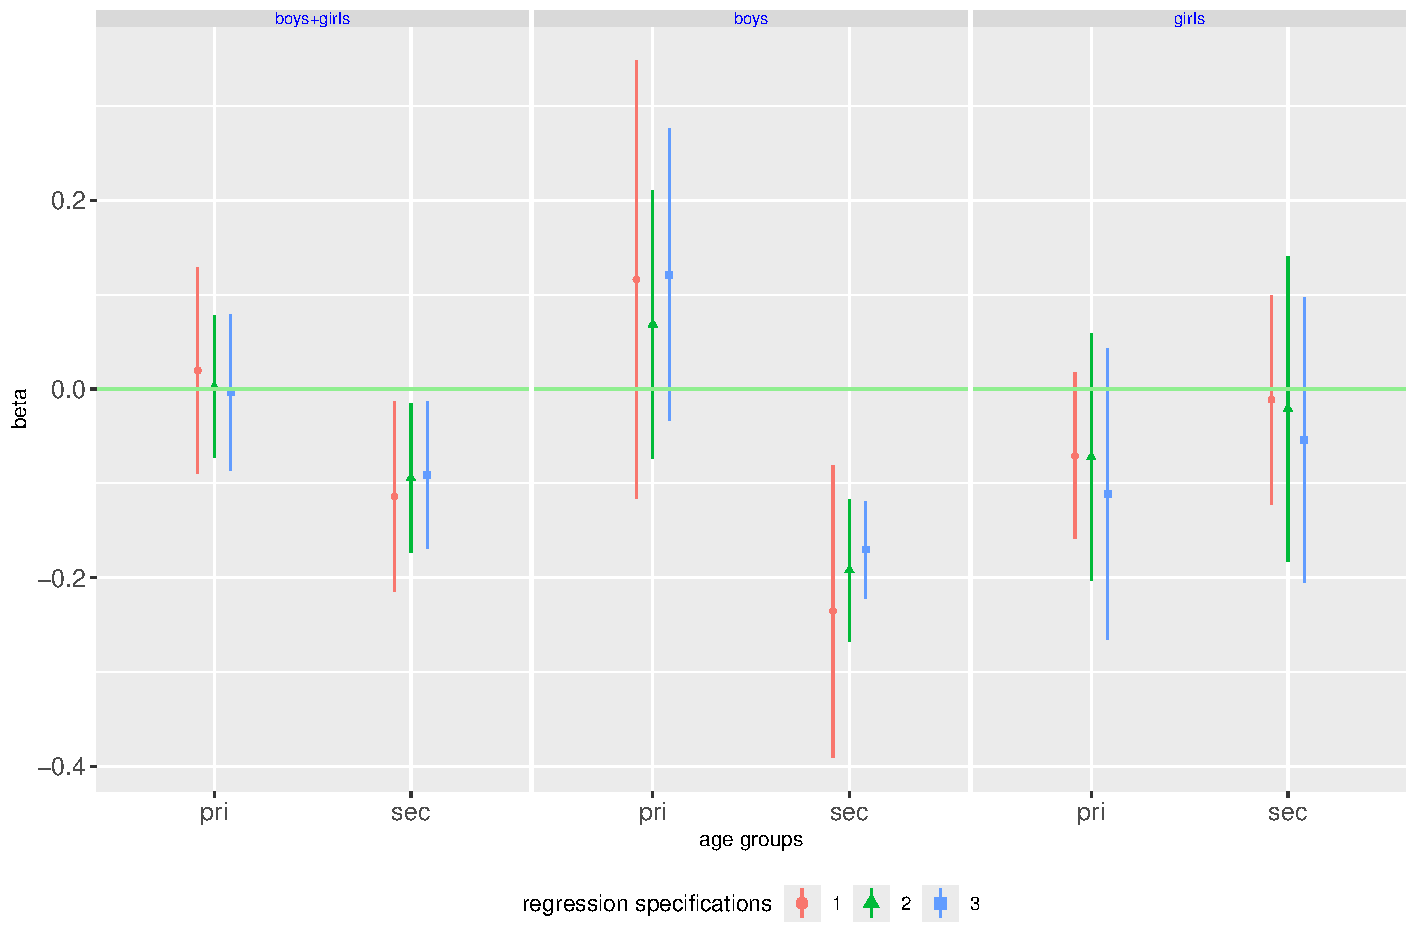
\includegraphics[height=.23\paperheight]{Figures/GenderAgeGroup2Impacts.pdf}\\
\renewcommand{\arraystretch}{1}
\hfil\begin{tabular}{>{\hfill\scriptsize}p{1cm}<{}>{\scriptsize}p{11cm}<{\hfill}}
Source: & Compiled from IFPRI data. \\[-1ex]
Notes:& 1. ``pri'' and ``sec'' mean enrolled in primary and secondary grades, aged 6-10 and 11-17 years in 1999, respectively. The coefficients are dummies for agri-HH $\times$ year 2002.\\[-1ex]
& 2. Specifications 1 - 3 correspond to the same specifications in \textsc{Table \ref{base10}}. \\[-1ex]
& 3. Error bars are 95\% confidence intervals using standard errors clustered at thana level with a Satterthwaite correction for small number of clusters.
\end{tabular}
%\end{minipage}
\end{figure}

\subsection{Placebo tests}

In this sub-section, we conduct placebo tests employing 2002-2006 panel data based on the fact that the 1999 favorable calendar returned to a normal (unfavorable) routine in 2002. Hence, the school enrollment rate should follow the common trend between the treatment and control groups, since there was no shift in the academic calendar between 2002 and 2006. We test this using two cohorts: 10-18 years old in 1999 (1999 cohort) and 10-18 years old in 2002 (2002 cohort). Given there is a significant sample overlap (13-18 in 2002), we treat the 2002 cohort as our main placebo check. 


\begin{table}\hfil\textsc{\footnotesize Table \refstepcounter{table}\thetable: Placebo estimation 2002-2006, 1999 and 2002 cohorts\label{Placebo10}}\\\setlength{\tabcolsep}{.5pt}\renewcommand{\arraystretch}{.675}\hspace{-2em}\hfil<<<<<<< HEAD
\begin{tabular}{>{\scriptsize}p{3cm}<{\hfill}>{\hfil\scriptsize$}p{1.3cm}<{$}>{\hfil\scriptsize$}p{1.3cm}<{$}>{\hfil\scriptsize$}p{1.3cm}<{$}>{$}p{0.1cm}<{$}>{\hfil\scriptsize$}p{1.3cm}<{$}>{\hfil\scriptsize$}p{1.3cm}<{$}>{\hfil\scriptsize$}p{1.3cm}<{$}>{$}p{0.1cm}<{$}>{\hfil\scriptsize$}p{1.3cm}<{$}>{\hfil\scriptsize$}p{1.3cm}<{$}>{\hfil\scriptsize$}p{1.3cm}<{$}}
\hline
\makebox[3cm]{\scriptsize\hfil }&\multicolumn{3}{c}{\makebox[3.9cm]{\scriptsize \textsf{Boys+Girls}}}&&\multicolumn{3}{c}{\makebox[3.9cm]{\scriptsize \textsf{Boys}}}&&\multicolumn{3}{c}{\makebox[2.7cm]{\scriptsize \textsf{Girls}}} \\[-.5ex]
\cline{2-4} \cline{6-8} \cline{10-12} \\[-1ex]
&\multicolumn{11}{c}{\scriptsize A. 2002 cohort}\\
\makebox[3cm]{rnm} & \makebox[1.3cm]{(1)} & \makebox[1.3cm]{(2)} & \makebox[1.3cm]{(3)} & \makebox[0.1cm]{} & \makebox[1.3cm]{(1)} & \makebox[1.3cm]{(2)} & \makebox[1.3cm]{(3)} & \makebox[0.1cm]{} & \makebox[1.3cm]{(1)} & \makebox[1.3cm]{(2)} & \makebox[1.3cm]{(3)}\\
Agricultural HH * year 2006 & -0.048^{\phantom{***}} & -0.023^{\phantom{***}} & -0.037^{\phantom{***}} &  & -0.004^{\phantom{***}} & -0.027^{\phantom{***}} & -0.045^{\phantom{***}} &  & -0.090^{\phantom{***}} & -0.029^{\phantom{***}} & -0.049^{\phantom{***}}\\[-1ex]
se$_{agHH.yr3}$ & (0.031)^{\phantom{**}} & (0.034)^{\phantom{**}} & (0.037)^{\phantom{**}} &  & (0.052)^{\phantom{**}} & (0.037)^{\phantom{**}} & (0.039)^{\phantom{**}} &  & (0.048)^{\phantom{**}} & (0.037)^{\phantom{**}} & (0.039)^{\phantom{**}}\\[-1ex]
 & {16.8}^{\phantom{**}} & {53.0}^{\phantom{**}} & {35.5}^{\phantom{**}} &  & {94.6}^{\phantom{**}} & {48.6}^{\phantom{**}} & {29.0}^{\phantom{**}} &  & {10.3}^{\phantom{**}} & {46.2}^{\phantom{**}} & {25.3}^{\phantom{**}}\\[-1ex]
 & \mbox{\tiny [-0.121, 0.026]} & \mbox{\tiny [-0.105, 0.060]} & \mbox{\tiny [-0.125, 0.052]} &  & \mbox{\tiny [-0.127, 0.120]} & \mbox{\tiny [-0.115, 0.061]} & \mbox{\tiny [-0.140, 0.049]} &  & \mbox{\tiny [-0.204, 0.024]} & \mbox{\tiny [-0.119, 0.060]} & \mbox{\tiny [-0.144, 0.045]}\\
$\underline{\phantom{mm}}$ * Older sisters &  &  & -0.073^{\phantom{***}} &  &  &  & -0.102^{\phantom{***}} &  &  &  & -0.046^{\phantom{***}}\\[-1ex]
se$_{OldSibF.agHH.yr3}$ &  &  & (0.037)^{\phantom{**}} &  &  &  & (0.053)^{\phantom{**}} &  &  &  & (0.036)^{\phantom{**}}\\[-1ex]
 &  &  & {10.4}^{\phantom{**}} &  &  &  & {10.7}^{\phantom{**}} &  &  &  & {26.4}^{\phantom{**}}\\[-1ex]
 &  &  & \mbox{\tiny [-0.167, 0.021]} &  &  &  & \mbox{\tiny [-0.234, 0.031]} &  &  &  & \mbox{\tiny [-0.140, 0.048]}\\
$\underline{\phantom{mm}}$ * Older brothers &  &  & 0.003^{\phantom{***}} &  &  &  & 0.042^{\phantom{***}} &  &  &  & -0.040^{\phantom{***}}\\[-1ex]
se$_{OldSibM.agHH.yr3}$ &  &  & (0.037)^{\phantom{**}} &  &  &  & (0.053)^{\phantom{**}} &  &  &  & (0.047)^{\phantom{**}}\\[-1ex]
 &  &  & {93.2}^{\phantom{**}} &  &  &  & {45.2}^{\phantom{**}} &  &  &  & {42.2}^{\phantom{**}}\\[-1ex]
 &  &  & \mbox{\tiny [-0.086, 0.093]} &  &  &  & \mbox{\tiny [-0.087, 0.172]} &  &  &  & \mbox{\tiny [-0.155, 0.074]}\\
$\bar{R}^{2}$ & 0.0025 & 0.2019 & 0.2197 &  & 0.0000 & 0.1128 & 0.1631 &  & 0.0086 & 0.3399 & 0.3688\\
N: agHH &  & 440 &  &  &  & 217 &  &  &  & 223 & \\
N &  & 812 &  &  &  & 386 &  &  &  & 426 & \\
mean of control in 2002 &  & 0.6747 &  &  &  & 0.6331 &  &  &  & 0.7094 & \\
mean of treated in 2002 &  & 0.5932 &  &  &  & 0.5438 &  &  &  & 0.6413 & \\
mean of control in 2006 &  & 0.4247 &  &  &  & 0.3787 &  &  &  & 0.4631 & \\
mean of treated in 2006 &  & 0.2955 &  &  &  & 0.2857 &  &  &  & 0.3049 & \\
=======
\begin{tabular}{>{\scriptsize}p{3.25cm}<{\hfill}>{\hfil\scriptsize$}p{1.5cm}<{$}>{\hfil\scriptsize$}p{1.5cm}<{$}>{\hfil\scriptsize$}p{1.5cm}<{$}>{$}p{0.1cm}<{$}>{\hfil\scriptsize$}p{1.5cm}<{$}>{\hfil\scriptsize$}p{1.5cm}<{$}>{\hfil\scriptsize$}p{1.5cm}<{$}>{$}p{0.1cm}<{$}>{\hfil\scriptsize$}p{1.5cm}<{$}>{\hfil\scriptsize$}p{1.5cm}<{$}>{\hfil\scriptsize$}p{1.5cm}<{$}}
\hline
\makebox[3.25cm]{\scriptsize\hfil }&\multicolumn{3}{c}{\makebox[4.5cm]{\scriptsize \textsf{Boys+Girls}}}&&\multicolumn{3}{c}{\makebox[4.5cm]{\scriptsize \textsf{Boys}}}&&\multicolumn{3}{c}{\makebox[3.1cm]{\scriptsize \textsf{Girls}}} \\[-.5ex]
\cline{2-4} \cline{6-8} \cline{10-12} \\[-1ex]
&\multicolumn{11}{c}{\scriptsize A. 2002 cohort}\\
  & (1) & (2) & (3) &  & (4) & (5) & (6) &  & (7) & (8) & (9) \\
Agricultural HH * year 2006 & -0.053^{\phantom{***}} & -0.030^{\phantom{***}} & -0.044^{\phantom{***}} &  & 0.004^{\phantom{***}} & -0.020^{\phantom{***}} & -0.029^{\phantom{***}} &  & -0.106^{*\phantom{**}} & -0.037^{\phantom{***}} & -0.049^{\phantom{***}}\\[-.5ex]
 & (14.2)^{\phantom{**}} & (40.6)^{\phantom{**}} & (35.7)^{\phantom{**}} &  & (93.5)^{\phantom{**}} & (57.9)^{\phantom{**}} & (35.6)^{\phantom{**}} &  & (7.9)^{\phantom{**}} & (44.4)^{\phantom{**}} & (49.3)^{\phantom{**}}\\[-.5ex]
 & \mbox{\tiny [-0.129, 0.023]} & \mbox{\tiny [-0.112, 0.051]} & \mbox{\tiny [-0.149, 0.062]} &  & \mbox{\tiny [-0.098, 0.105]} & \mbox{\tiny [-0.100, 0.061]} & \mbox{\tiny [-0.098, 0.041]} &  & \mbox{\tiny [-0.228, 0.016]} & \mbox{\tiny [-0.147, 0.073]} & \mbox{\tiny [-0.213, 0.114]}\\
$\underline{\phantom{mm}}$ * Older sisters &  &  & -0.071^{*\phantom{**}} &  &  &  & -0.098^{\phantom{***}} &  &  &  & -0.050^{\phantom{***}}\\[-.5ex]
 &  &  & (6.4)^{\phantom{**}} &  &  &  & (13.7)^{\phantom{**}} &  &  &  & (20.3)^{\phantom{**}}\\[-.5ex]
 &  &  & \mbox{\tiny [-0.148, 0.006]} &  &  &  & \mbox{\tiny [-0.239, 0.043]} &  &  &  & \mbox{\tiny [-0.139, 0.039]}\\
$\underline{\phantom{mm}}$ * Older brothers &  &  & 0.012^{\phantom{***}} &  &  &  & 0.077^{\phantom{***}} &  &  &  & -0.044^{\phantom{***}}\\[-.5ex]
 &  &  & (71.9)^{\phantom{**}} &  &  &  & (13.3)^{\phantom{**}} &  &  &  & (31.2)^{\phantom{**}}\\[-.5ex]
 &  &  & \mbox{\tiny [-0.069, 0.094]} &  &  &  & \mbox{\tiny [-0.033, 0.186]} &  &  &  & \mbox{\tiny [-0.143, 0.055]}\\
$\bar{R}^{2}$ & 0.0030 & 0.2022 & 0.2250 &  & 0.0000 & 0.1124 & 0.1738 &  & 0.0115 & 0.3404 & 0.3635\\
N: agHH &  & 492 &  &  &  & 243 &  &  &  & 249 & \\
N &  & 812 &  &  &  & 386 &  &  &  & 426 & \\
mean of control in 2002 &  & 0.6844 &  &  &  & 0.6573 &  &  &  & 0.7062 & \\
mean of treated in 2002 &  & 0.5955 &  &  &  & 0.5391 &  &  &  & 0.6506 & \\
mean of control in 2006 &  & 0.4406 &  &  &  & 0.3986 &  &  &  & 0.4746 & \\
mean of treated in 2006 &  & 0.2988 &  &  &  & 0.2840 &  &  &  & 0.3133 & \\
>>>>>>> 41dec8f560b653fb2373d27136c157ebc2dfddbe
\multicolumn{12}{l}{\scriptsize Common specifications}\\
\hspace{.5em}Covariates, thana trends &  & \mbox{Y} & \mbox{Y} &  &  & \mbox{Y} & \mbox{Y} &  &  & \mbox{Y} & \mbox{Y}\\
\hspace{.5em}HH trends &  &  & \mbox{Y} &  &  &  & \mbox{Y} &  &  &  & \mbox{Y}\\
&\multicolumn{11}{c}{\scriptsize B. 1999 cohort}\\
<<<<<<< HEAD
&(10)&(11)&(12)&(13)&(14)&(15)&(16)&(17)&(18) \\
Agricultural HH * year 2006 & -0.022^{\phantom{***}} & -0.028^{\phantom{***}} & -0.034^{\phantom{***}} &  & 0.019^{\phantom{***}} & -0.011^{\phantom{***}} & -0.017^{\phantom{***}} &  & -0.070^{\phantom{***}} & -0.047^{\phantom{***}} & -0.066^{\phantom{***}}\\[-1ex]
se$_{agHH.yr3}$ & (0.043)^{\phantom{**}} & (0.029)^{\phantom{**}} & (0.031)^{\phantom{**}} &  & (0.061)^{\phantom{**}} & (0.047)^{\phantom{**}} & (0.046)^{\phantom{**}} &  & (0.064)^{\phantom{**}} & (0.042)^{\phantom{**}} & (0.045)^{\phantom{**}}\\[-1ex]
 & {63.3}^{\phantom{**}} & {37.9}^{\phantom{**}} & {31.4}^{\phantom{**}} &  & {76.1}^{\phantom{**}} & {81.7}^{\phantom{**}} & {72.4}^{\phantom{**}} &  & {31.1}^{\phantom{**}} & {31.0}^{\phantom{**}} & {19.0}^{\phantom{**}}\\[-1ex]
 & \mbox{\tiny [-0.125, 0.082]} & \mbox{\tiny [-0.099, 0.043]} & \mbox{\tiny [-0.110, 0.041]} &  & \mbox{\tiny [-0.126, 0.164]} & \mbox{\tiny [-0.123, 0.100]} & \mbox{\tiny [-0.129, 0.095]} &  & \mbox{\tiny [-0.224, 0.084]} & \mbox{\tiny [-0.151, 0.057]} & \mbox{\tiny [-0.177, 0.044]}\\
$\underline{\phantom{mm}}$ * Older sisters &  &  & -0.070^{\phantom{***}} &  &  &  & -0.006^{\phantom{***}} &  &  &  & -0.081^{\phantom{***}}\\[-1ex]
se$_{OldSibF.agHH.yr3}$ &  &  & (0.042)^{\phantom{**}} &  &  &  & (0.045)^{\phantom{**}} &  &  &  & (0.082)^{\phantom{**}}\\[-1ex]
 &  &  & {16.0}^{\phantom{**}} &  &  &  & {90.0}^{\phantom{**}} &  &  &  & {37.1}^{\phantom{**}}\\[-1ex]
 &  &  & \mbox{\tiny [-0.180, 0.040]} &  &  &  & \mbox{\tiny [-0.121, 0.109]} &  &  &  & \mbox{\tiny [-0.299, 0.137]}\\
$\underline{\phantom{mm}}$ * Older brothers &  &  & -0.009^{\phantom{***}} &  &  &  & 0.002^{\phantom{***}} &  &  &  & -0.044^{\phantom{***}}\\[-1ex]
se$_{OldSibM.agHH.yr3}$ &  &  & (0.052)^{\phantom{**}} &  &  &  & (0.076)^{\phantom{**}} &  &  &  & (0.055)^{\phantom{**}}\\[-1ex]
 &  &  & {86.6}^{\phantom{**}} &  &  &  & {98.0}^{\phantom{**}} &  &  &  & {46.0}^{\phantom{**}}\\[-1ex]
 &  &  & \mbox{\tiny [-0.140, 0.121]} &  &  &  & \mbox{\tiny [-0.191, 0.195]} &  &  &  & \mbox{\tiny [-0.182, 0.094]}\\
$\bar{R}^{2}$ & 0.0005 & 0.2928 & 0.3199 &  & 0.0005 & 0.1052 & 0.1515 &  & 0.0054 & 0.4885 & 0.5218\\
N: agHH &  & 341 &  &  &  & 176 &  &  &  & 165 & \\
N &  & 616 &  &  &  & 304 &  &  &  & 312 & \\
mean of control in 2002 &  & 0.4909 &  &  &  & 0.4453 &  &  &  & 0.5306 & \\
mean of treated in 2002 &  & 0.3783 &  &  &  & 0.2898 &  &  &  & 0.4727 & \\
mean of control in 2006 &  & 0.2691 &  &  &  & 0.2500 &  &  &  & 0.2857 & \\
mean of treated in 2006 &  & 0.1349 &  &  &  & 0.1136 &  &  &  & 0.1576 & \\
=======
  & (10) & (11) & (12) &  & (13) & (14) & (15) &  & (16) & (17) & (18) \\
Agricultural HH * year 2006 & -0.023^{\phantom{***}} & -0.031^{\phantom{***}} & -0.033^{\phantom{***}} &  & 0.030^{\phantom{***}} & 0.007^{\phantom{***}} & 0.001^{\phantom{***}} &  & -0.084^{\phantom{***}} & -0.058^{\phantom{***}} & -0.069^{\phantom{***}}\\[-.5ex]
 & (61.1)^{\phantom{**}} & (22.9)^{\phantom{**}} & (39.5)^{\phantom{**}} &  & (55.0)^{\phantom{**}} & (87.2)^{\phantom{**}} & (98.7)^{\phantom{**}} &  & (27.5)^{\phantom{**}} & (28.1)^{\phantom{**}} & (27.8)^{\phantom{**}}\\[-.5ex]
 & \mbox{\tiny [-0.128, 0.082]} & \mbox{\tiny [-0.088, 0.026]} & \mbox{\tiny [-0.120, 0.054]} &  & \mbox{\tiny [-0.086, 0.146]} & \mbox{\tiny [-0.101, 0.116]} & \mbox{\tiny [-0.114, 0.116]} &  & \mbox{\tiny [-0.256, 0.087]} & \mbox{\tiny [-0.177, 0.062]} & \mbox{\tiny [-0.212, 0.074]}\\
$\underline{\phantom{mm}}$ * Older sisters &  &  & -0.053^{\phantom{***}} &  &  &  & 0.015^{\phantom{***}} &  &  &  & -0.097^{\phantom{***}}\\[-.5ex]
 &  &  & (36.5)^{\phantom{**}} &  &  &  & (83.8)^{\phantom{**}} &  &  &  & (25.0)^{\phantom{**}}\\[-.5ex]
 &  &  & \mbox{\tiny [-0.195, 0.089]} &  &  &  & \mbox{\tiny [-0.167, 0.196]} &  &  &  & \mbox{\tiny [-0.295, 0.100]}\\
$\underline{\phantom{mm}}$ * Older brothers &  &  & -0.003^{\phantom{***}} &  &  &  & 0.033^{\phantom{***}} &  &  &  & -0.038^{\phantom{***}}\\[-.5ex]
 &  &  & (96.1)^{\phantom{**}} &  &  &  & (65.4)^{\phantom{**}} &  &  &  & (42.2)^{\phantom{**}}\\[-.5ex]
 &  &  & \mbox{\tiny [-0.129, 0.124]} &  &  &  & \mbox{\tiny [-0.154, 0.221]} &  &  &  & \mbox{\tiny [-0.150, 0.075]}\\
$\bar{R}^{2}$ & 0.0006 & 0.2930 & 0.3208 &  & 0.0011 & 0.1051 & 0.1628 &  & 0.0076 & 0.4895 & 0.5205\\
N: agHH &  & 379 &  &  &  & 196 &  &  &  & 183 & \\
N &  & 616 &  &  &  & 304 &  &  &  & 312 & \\
mean of control in 2002 &  & 0.4979 &  &  &  & 0.4722 &  &  &  & 0.5194 & \\
mean of treated in 2002 &  & 0.3852 &  &  &  & 0.2908 &  &  &  & 0.4863 & \\
mean of control in 2006 &  & 0.2785 &  &  &  & 0.2685 &  &  &  & 0.2868 & \\
mean of treated in 2006 &  & 0.1425 &  &  &  & 0.1173 &  &  &  & 0.1694 & \\
>>>>>>> 41dec8f560b653fb2373d27136c157ebc2dfddbe
\multicolumn{12}{l}{\scriptsize Common specifications}\\
\hspace{.5em}Covariates, thana trends &  & \mbox{Y} & \mbox{Y} &  &  & \mbox{Y} & \mbox{Y} &  &  & \mbox{Y} & \mbox{Y}\\
\hspace{.5em}HH trends &  &  & \mbox{Y} &  &  &  & \mbox{Y} &  &  &  & \mbox{Y}\\
\hline
\end{tabular}
\\\renewcommand{\arraystretch}{1}\hfil\begin{tabular}{>{\hfill\scriptsize}p{1cm}<{}>{\scriptsize}p{12cm}<{\hfill}} Source:& Compiled from IFPRI data. \\[-1ex] Notes:&   \textsf{Agricultural HH * year 2002} is an interaction term of agricultural household dummy and year 2002 dummy. All interaction terms are demeaned. For each panel, first columns are raw DID. Second columns add time-varying thana level characteristics (yield, mean rainfall, mean high temperature, mean low temperature), individual level characteristics (age squared, recipient of a poverty program), and \textsf{Thana trends} that are interactions of year 2002 dummy with Thana fixed effects. Third columns add interactions of year 2002 dummy and individual level characterstics (sex of individual, household head's and spouse's education, number of older male/female siblings, per member land holding, per member non land asset holding, piped water access, structured toilet access) $\bfx_{i}r_{t}$, and triple interactions of year 2002 dummy, individual characteristics, and agricultural household dummy $\bfx_{i}r_{t}D_{i}$. Rows of $\underline{\phantom{mm}}*x$ show estimates of the triple interaction term of $x_{i}$, or $x_{i}r_{t}D_{i}$. Parental education variables are strongly collinear with agricultural household dummy and are used only in year 2002 interaction terms to avoid multicollinearity.   \end{tabular} \end{table}

Table \ref{Placebo10} provides the results of two sets of placebo tests. All regression specifications follow those of \textsc{Table \ref{base10}}. In Panel A, we report the first placebo test using 10-18-year-old in 2002 (2002 cohort). Our coefficient of interest $\hat{\gamma}$ has a smaller point estimate relative to the main results with larger standard errors, leading to large $p$ values.\footnote{The point estimates are all negative, indicating children from agricultural households tend to drop out earlier even when exam-harvest overlap is absent. Consistent with our brawn-based interpretation that female labor is not a perfect substitute for male labor to work in the field, we obtain negative estimates on the triple interaction terms of the number of older female siblings with $p$ values ranging between 7.2\% and 8.9\%. This implies that children from agricultural households are naturally disadvantaged in schooling even if there is no change in exam-harvest overlap when the household demographic structure is unfavorable. } The estimation results using gender subsamples are also similar. The second set of tests in Panel B. use the same individuals (10-18 years old in 1999) as the main estimation but observed in the later rounds of data. Most of the estimates are negative but statistically indistinguishable from zero. 

The most encouraging evidence in our placebo tests is found in the boys susample that shows null effects. In the main results, the boys subsample was estimated to be most affected by the harvest labor demand of 2002. If this was confounded by some other factor that are unrelated to exam schedule change, we should detect the similar effects in the placebo testing of 2002-2006. The fact that boys subsample of agricultural and non-agricultural households show the common trend is consistent with our interpretation that the exam schedule conflict with harvesting season is pulling students out from school. In addition, this is also consistent with the common trend assumption we use in DID between the agricultural and non-agricultural households. 



\subsection{Secondary Outcomes}

In \textsc{\small Table \ref{NumGradesDaysAbsentResults}}, we examine the impacts on secondary outcomes related to enrollment continuation: The number of completed grades or grade progression in three years (between 1999-2002),\footnote{Grade progression is defined as the difference in reported grades between 2002 and 1999 for individuals who are not out of school. Out-of-school individuals are those whose schooling is lower than grade 1, who are not enrolled in both 1999 and 2002 rounds, or who are not reporting a change in grade between 1999 and 2002. } and the mean number of days absent from school in the past three months before the survey interview date (July-August 1999 and 2002). Outcome measures are estimated for those enrolled in 1999 (panel A of Table \ref{NumGradesDaysAbsentResults}), those enrolled in both the 1999 and 2002 rounds (panels B-D of Table \ref{NumGradesDaysAbsentResults}). These exercises use the samples of children, 10 - 18 years old, enrolled in 1999, so the estimated impacts are conditional on enrollment in 1999.

Columns (1)-(3) show the negative impacts on grade progression among children from agricultural households in 2002 when the academic calendar was unfavorable. This negative grade progression estimates range from -0.46 to -0.48 years (from the base of 2.08 years of progression by the non-agricultural household children). We interpret these are one year effect of 2002, because the calendar was favorable up to 2001 and any negative effects should be only of year 2002. 
In columns (4)-(6) of the panel B sample, the estimates are similar, however smaller in magnitude, which is reasonable given that the sample used in panel A includes dropouts in 2002 who have fewer grade progression. This implies that agricultural children struggle to get ``passing'' scores to continue academic progression, which could be related to inadequate learning owing to school absenteeism, particularly during the peak labor demand season. 

Given we use the sample of enrollers, slower grade progression is added on top of the higher dropout rates of agricultural households. Even when the children of agricultural houseshold manage to stay on school, they learn more slowly than the children of non-agricultural households. This is an additional cost on human capital investments for children facing local agricultural labor demand.

Columns (7)-(9) present the estimates of the impacts on the average monthly absent days for students enrolled in both survey rounds. Impacts range from 0.68 to 0.98 day per month, which is small in magnitude, although estimated precisely even with small sample size. 

In columns (10)-(12), the sample consists of continuing school students and uses only the cross-section sample of 1999 (asked on absence of 2000 in 2000). Columns (10)-(12), the sample consists of continuing school students and uses only the cross-section sample of 2002 (asked on absence of 2003 in 2003). We use two cross section samples in these estimates to see if the labor demand increase may affect absence. In both samples, the survey asked about the absence during the planting season. In the year 2000 sample, we see zero impacts. Point estimates are small and change the signs by specification, and $p$ values are large. In the 2003 sample, the point estimates are positive and larger, with the $p$ values ranging between 10.5 to 17.6\%. This shows that children of agricultural households were more absent in the planting season of 2003, but not so in the planting season of 2000. This is consistent with the decision that having a favorable final exam schedule in 2000 induced the students not to go to planting work, while they went to planting work in 2003 when the final exam schedule was unfavorable. We interpret the results as an indication that children are forward looking that the regular school attendance in the months well before final exam schedule can also be affected. 

\begin{table}\hfil\textsc{\footnotesize Table \refstepcounter{table}\thetable: Other schooling outcomes, grade progression and days absent\label{NumGradesDaysAbsentResults}}\\\setlength{\tabcolsep}{.5pt}\renewcommand{\arraystretch}{.675}\hspace{-2em}\hfil\begin{tabular}{>{\scriptsize}p{3.25cm}<{\hfill}>{\hfil\scriptsize$}p{1.5cm}<{$}>{\hfil\scriptsize$}p{1.5cm}<{$}>{\hfil\scriptsize$}p{1.5cm}<{$}>{$}p{0.1cm}<{$}>{\hfil\scriptsize$}p{1.5cm}<{$}>{\hfil\scriptsize$}p{1.5cm}<{$}>{\hfil\scriptsize$}p{1.5cm}<{$}}
\hline
\makebox[3.25cm]{\scriptsize\hfil }&\multicolumn{3}{c}{\makebox[4.5cm]{\scriptsize \textsf{Grade progression}}}&&\multicolumn{3}{c}{\makebox[4.5cm]{\scriptsize \textsf{Days absent}}} \\[-.5ex]
\cline{2-4} \cline{6-8} \\[-1ex]
&\multicolumn{7}{c}{\scriptsize A. Students enrolled in 1999}\\
&(1)&(2)&(3)&&&&\\
\hspace{.5em}Agricultural HH & -0.443^{***} & -0.464^{**\phantom{*}} & -0.471^{**\phantom{*}} &  &  &  & \\[-1ex]
se$_{agHH.yr2}$ & (0.107)^{\phantom{**}} & (0.125)^{\phantom{**}} & (0.136)^{\phantom{**}} &  &  &  & \\[-1ex]
 & {0.5}^{\phantom{**}} & {1.1}^{\phantom{**}} & {1.4}^{\phantom{**}} &  &  &  & \\[-1ex]
 & \mbox{\tiny [-0.700, -0.186]} & \mbox{\tiny [-0.774, -0.153]} & \mbox{\tiny [-0.805, -0.137]} &  &  &  & \\[-1ex]
 &  & \mbox{\tiny [0.572, 1.430]} & \mbox{\tiny [0.647, 1.501]} &  &  &  & \\[-1ex]
 &  & \mbox{\tiny [0.531, 1.607]} & \mbox{\tiny [0.637, 1.775]} &  &  &  & \\
$\bar{R}^{2}$ & 0.0251 & 0.2614 & 0.2942 &  &  &  & \\
N: agHH &  & 210 &  &  &  &  & \\
N &  & 393 &  &  &  &  & \\
mean of control in 1999 &  & 5.1585 &  &  &  &  & \\
mean of treated in 1999 &  & 5.0476 &  &  &  &  & \\
mean of control in 2002 &  & 7.2732 &  &  &  &  & \\
mean of treated in 2002 &  & 6.7190 &  &  &  &  & \\
&\multicolumn{7}{c}{\scriptsize B. Students enrolled in 1999 and 2002}\\
&(4)&(5)&(6)&&(7)&(8)&(9)\\
\hspace{.5em}Agricultural HH & -0.189^{*\phantom{**}} & -0.231^{\phantom{***}} & -0.269^{**\phantom{*}} &  & 0.562^{\phantom{***}} & 0.815^{\phantom{***}} & 0.766^{\phantom{***}}\\[-1ex]
se$_{agHH.yr2}$ & (0.097)^{\phantom{**}} & (0.119)^{\phantom{**}} & (0.077)^{\phantom{**}} &  & (0.396)^{\phantom{**}} & (0.423)^{\phantom{**}} & (0.553)^{\phantom{**}}\\[-1ex]
 & {9.6}^{\phantom{**}} & {10.2}^{\phantom{**}} & {1.3}^{\phantom{**}} &  & {20.3}^{\phantom{**}} & {10.3}^{\phantom{**}} & {21.5}^{\phantom{**}}\\[-1ex]
 & \mbox{\tiny [-0.422, 0.044]} & \mbox{\tiny [-0.523, 0.062]} & \mbox{\tiny [-0.456, -0.081]} &  & \mbox{\tiny [-0.391, 1.515]} & \mbox{\tiny [-0.226, 1.857]} & \mbox{\tiny [-0.584, 2.116]}\\[-1ex]
 &  & \mbox{\tiny [0.161, 1.232]} & \mbox{\tiny [0.388, 1.320]} &  &  & \mbox{\tiny [-1.721, 0.824]} & \mbox{\tiny [-2.348, 0.088]}\\[-1ex]
 &  & \mbox{\tiny [0.419, 1.595]} & \mbox{\tiny [0.603, 1.738]} &  &  & \mbox{\tiny [-2.102, 2.695]} & \mbox{\tiny [-2.806, 1.596]}\\
$\bar{R}^{2}$ & 0.0064 & 0.2146 & 0.2565 &  & 0.0042 & 0.0665 & 0.1447\\
N: agHH &  & 126 &  &  &  & 129 & \\
N &  & 260 &  &  &  & 263 & \\
mean of control in 1999 &  & 4.9776 &  &  &  & 3.4030 & \\
mean of treated in 1999 &  & 4.7381 &  &  &  & 3.3437 & \\
mean of control in 2002 &  & 7.3731 &  &  &  & 3.0672 & \\
mean of treated in 2002 &  & 6.9444 &  &  &  & 3.5698 & \\
&\multicolumn{7}{c}{\scriptsize C. Students enrolled in 1999 and 2002, cross section OLS of 2000}\\
&&&&&(10)&(11)&(12)\\
Agricultural HH &  &  &  &  & -0.059^{\phantom{***}} & -0.258^{\phantom{***}} & -0.234^{\phantom{***}}\\[-1ex]
se$_{agHH}$ &  &  &  &  & (0.245)^{\phantom{**}} & (0.287)^{\phantom{**}} & (0.302)^{\phantom{**}}\\[-1ex]
 &  &  &  &  & {81.6}^{\phantom{**}} & {40.4}^{\phantom{**}} & {46.9}^{\phantom{**}}\\[-1ex]
 &  &  &  &  & \mbox{\tiny [-0.647, 0.529]} & \mbox{\tiny [-0.965, 0.448]} & \mbox{\tiny [-0.977, 0.510]}\\[-1ex]
 &  &  &  &  &  & \mbox{\tiny [-2.485, 0.861]} & \mbox{\tiny [-2.280, 0.796]}\\
$\bar{R}^{2}$ &  &  &  &  & 0.0001 & 0.0452 & 0.1814\\
N: agHH &  &  &  &  &  & 129 & \\
N &  &  &  &  &  & 263 & \\
mean of control in 1999 &  &  &  &  &  & 3.4030 & \\
mean of treated in 1999 &  &  &  &  &  & 3.3437 & \\
&\multicolumn{7}{c}{\scriptsize D. Students enrolled in 1999 and 2002, cross section OLS of 2003}\\
&&&&&(13)&(14)&(15)\\
Agricultural HH &  &  &  &  & 0.503^{\phantom{***}} & 0.574^{\phantom{***}} & 0.495^{\phantom{***}}\\[-1ex]
se$_{agHH}$ &  &  &  &  & (0.419)^{\phantom{**}} & (0.524)^{\phantom{**}} & (0.469)^{\phantom{**}}\\[-1ex]
 &  &  &  &  & {27.2}^{\phantom{**}} & {31.6}^{\phantom{**}} & {33.2}^{\phantom{**}}\\[-1ex]
 &  &  &  &  & \mbox{\tiny [-0.504, 1.509]} & \mbox{\tiny [-0.714, 1.863]} & \mbox{\tiny [-0.654, 1.644]}\\[-1ex]
 &  &  &  &  &  & \mbox{\tiny [-1.866, 0.652]} & \mbox{\tiny [-2.260, 0.461]}\\
$\bar{R}^{2}$ &  &  &  &  & 0.0053 & 0.0593 & 0.1816\\
N: agHH &  &  &  &  &  & 129 & \\
N &  &  &  &  &  & 263 & \\
mean of control in 2002 &  &  &  &  &  & 3.0672 & \\
mean of treated in 2002 &  &  &  &  &  & 3.5698 & \\
\multicolumn{8}{l}{\scriptsize Common specifications}\\
\hspace{.5em}Covariates, thana trends &  &  & \mbox{Y} &  &  &  & \mbox{Y}\\
\hspace{.5em}HH trends &  &  & \mbox{Y} &  &  &  & \mbox{Y}\\
\hline
\end{tabular}
\\\renewcommand{\arraystretch}{1}\hfil\begin{tabular}{>{\hfill\scriptsize}p{1cm}<{}>{\scriptsize}p{12cm}<{\hfill}} Source:& Compiled from IFPRI data. \\[-1ex] Notes:&   \textsf{Agricultural HH * year 2002} is an interaction term of agricultural household dummy and year 2002 dummy. All interaction terms are demeaned. For each panel, first columns are raw DID. Second columns add time-varying thana level characteristics (yield, mean rainfall, mean high temperature, mean low temperature), individual level characteristics (age squared, recipient of a poverty program), and \textsf{Thana trends} that are interactions of year 2002 dummy with Thana fixed effects. Third columns add interactions of year 2002 dummy and individual level characterstics (sex of individual, household head's and spouse's education, number of older male/female siblings, per member land holding, per member non land asset holding, piped water access, structured toilet access) $\bfx_{i}r_{t}$, and triple interactions of year 2002 dummy, individual characteristics, and agricultural household dummy $\bfx_{i}r_{t}D_{i}$. Rows of $\underline{\phantom{mm}}*x$ show estimates of the triple interaction term of $x_{i}$, or $x_{i}r_{t}D_{i}$. Parental education variables are strongly collinear with agricultural household dummy and are used only in year 2002 interaction terms to avoid multicollinearity., \\   \end{tabular} \end{table}

Our estimates indicate that children from agricultural households systematically missed more (about 28\%) school days, on average, during July-August, which overlaps with the local \textit{Aman} paddy planting time (see section \ref{sec.rice}). Gender sub-sample estimation (reported in Appendix Table X) shows this absenteeism impact predominantly comes from boys. On average, boys from agricultural households missed school about 1.2-2.5 days more per month in 2002 during the planting time (from the base of 2.5 absent days for non-agriculture household students, an increment equivalent to 48-100\%). 

Taken together, these results suggest that learning, when measured by regular school attendance, is affected by local agricultural activities. This provides plausible evidence that absenteeism hinders grade progression and school continuation, particularly when the annual exam is held during the harvesting season.

\subsection{Testing for alternative mechanisms}

In Table \ref{FloodNonMuslimResultsConcise}, we report two tests to check the plausibility of alternative mechanisms that are consistent with the estimated results: Non-Muslims and flood-affected areas. 

It is possible that our estimates primarily capture the impact of fasting and festivities during \textit{Ramadan}, which may diminish children's capacity to learn and pass annual exams. To verify this empirically, we compare Muslim and non-Muslim households. As non-Muslims do not fast and are less prone to be affected by festivities, this exercise helps us disentangle the impact of festivities. Columns (1)-(3) of Table \ref{FloodNonMuslimResultsConcise} present estimates using a non-Muslim dummy and its interaction with the year 2002 and the year 2002*agricultural household. We can observe that our main coefficient of interest does not differ from those in Table \ref{base10}. For non-Muslims, the statistically imprecise point estimates suggest that \textit{Ramadan} before the exam in 2002, fasting before the final exams, and post-\textit{Ramadan} festivities are not plausible mechanisms leading to lower enrollment rates for children from agricultural households.

\begin{table}\hfil\textsc{\footnotesize Table \refstepcounter{table}\thetable: Alternative mechanisms, flood and non-Muslims\label{FloodNonMuslimResultsConcise}}\\\setlength{\tabcolsep}{.5pt}\renewcommand{\arraystretch}{.675}\hspace{-2em}\hfil\begin{tabular}{>{\scriptsize}p{3.25cm}<{\hfill}>{\hfil\scriptsize$}p{1.5cm}<{$}>{\hfil\scriptsize$}p{1.5cm}<{$}>{\hfil\scriptsize$}p{1.5cm}<{$}>{$}p{0.1cm}<{$}>{\hfil\scriptsize$}p{1.5cm}<{$}>{\hfil\scriptsize$}p{1.5cm}<{$}>{\hfil\scriptsize$}p{1.5cm}<{$}>{$}p{0.1cm}<{$}>{\hfil\scriptsize$}p{1.5cm}<{$}>{\hfil\scriptsize$}p{1.5cm}<{$}>{\hfil\scriptsize$}p{1.5cm}<{$}}
\hline
\makebox[3.25cm]{\scriptsize\hfil }&\multicolumn{3}{c}{\makebox[4.5cm]{\scriptsize \textsf{Boys+girls}}}&&\multicolumn{3}{c}{\makebox[4.5cm]{\scriptsize \textsf{Boys}}}&&\multicolumn{3}{c}{\makebox[3.1cm]{\scriptsize \textsf{Girls}}} \\[-.5ex]
\cline{2-4} \cline{6-8} \cline{10-12} \\[-1ex]
&\multicolumn{11}{c}{\scriptsize A. Non Muslims}\\
\makebox[3.25cm]{Covariates}&\makebox[1.3cm]{(1)}&\makebox[1.3cm]{(2)}&\makebox[1.3cm]{(3)}&&\makebox[1.3cm]{(4)}&\makebox[1.3cm]{(5)}&\makebox[1.3cm]{(6)}&&\makebox[1.3cm]{(7)}&\makebox[1.3cm]{(8)}&\makebox[1.3cm]{(9)}\\
Agricultural HH * year 2002 & -0.090^{*\phantom{**}} & -0.085^{**\phantom{*}} & -0.085^{**\phantom{*}} &  & -0.175^{*\phantom{**}} & -0.162^{***} & -0.148^{***} &  & -0.010^{\phantom{***}} & -0.025^{\phantom{***}} & -0.042^{\phantom{***}}\\[-1ex]
se$_{agHH.yr2}$ & (0.045)^{\phantom{**}} & (0.024)^{\phantom{**}} & (0.033)^{\phantom{**}} &  & (0.081)^{\phantom{**}} & (0.041)^{\phantom{**}} & (0.019)^{\phantom{**}} &  & (0.045)^{\phantom{**}} & (0.066)^{\phantom{**}} & (0.064)^{\phantom{**}}\\[-1ex]
 & {8.8}^{\phantom{**}} & {1.1}^{\phantom{**}} & {4.0}^{\phantom{**}} &  & {6.9}^{\phantom{**}} & {0.7}^{\phantom{**}} & {0.0}^{\phantom{**}} &  & {83.8}^{\phantom{**}} & {71.7}^{\phantom{**}} & {53.1}^{\phantom{**}}\\[-1ex]
 & \mbox{\tiny [-0.197, 0.018]} & \mbox{\tiny [-0.143, -0.027]} & \mbox{\tiny [-0.164, -0.005]} &  & \mbox{\tiny [-0.368, 0.019]} & \mbox{\tiny [-0.261, -0.063]} & \mbox{\tiny [-0.196, -0.101]} &  & \mbox{\tiny [-0.119, 0.100]} & \mbox{\tiny [-0.186, 0.136]} & \mbox{\tiny [-0.199, 0.114]}\\
Non-Muslim * year 2002 &  & 0.072^{\phantom{***}} & 0.074^{\phantom{***}} &  &  & 0.123^{\phantom{***}} & 0.087^{\phantom{***}} &  &  & 0.065^{\phantom{***}} & 0.089^{\phantom{***}}\\[-1ex]
se$_{nonmuslim.yr2}$ &  & (0.059)^{\phantom{**}} & (0.041)^{\phantom{**}} &  &  & (0.090)^{\phantom{**}} & (0.051)^{\phantom{**}} &  &  & (0.052)^{\phantom{**}} & (0.067)^{\phantom{**}}\\[-1ex]
 &  & {30.6}^{\phantom{**}} & {15.9}^{\phantom{**}} &  &  & {27.0}^{\phantom{**}} & {17.8}^{\phantom{**}} &  &  & {28.6}^{\phantom{**}} & {25.8}^{\phantom{**}}\\[-1ex]
 &  & \mbox{\tiny [-0.109, 0.252]} & \mbox{\tiny [-0.048, 0.196]} &  &  & \mbox{\tiny [-0.176, 0.423]} & \mbox{\tiny [-0.065, 0.238]} &  &  & \mbox{\tiny [-0.086, 0.216]} & \mbox{\tiny [-0.102, 0.280]}\\
$\underline{\phantom{mm}}$ * Ag HH &  & 0.035^{\phantom{***}} & 0.010^{\phantom{***}} &  &  & -0.173^{\phantom{***}} & -0.240^{\phantom{***}} &  &  & 0.128^{\phantom{***}} & 0.124^{\phantom{***}}\\[-1ex]
$\bar{R}^{2}$ & 0.0085 & 0.4700 & 0.4889 &  & 0.0328 & 0.3804 & 0.4384 &  & 0.0001 & 0.5959 & 0.6168\\
N: Muslims &  & 77 &  &  &  & 36 &  &  &  & 41 & \\
N &  & 626 &  &  &  & 306 &  &  &  & 320 & \\
mean of control in 1999 &  & 0.7464 &  &  &  & 0.6512 &  &  &  & 0.8278 & \\
mean of treated in 1999 &  & 0.7312 &  &  &  & 0.6780 &  &  &  & 0.7870 & \\
mean of control in 2002 &  & 0.4893 &  &  &  & 0.4419 &  &  &  & 0.5298 & \\
&\multicolumn{11}{c}{\scriptsize B. Flooded}\\
\makebox[3.25cm]{Covariates}&\makebox[1.3cm]{(10)}&\makebox[1.3cm]{(11)}&\makebox[1.3cm]{(12)}&&\makebox[1.3cm]{(13)}&\makebox[1.3cm]{(14)}&\makebox[1.3cm]{(15)}&&\makebox[1.3cm]{(16)}&\makebox[1.3cm]{(17)}&\makebox[1.3cm]{(18)}\\
Agricultural HH * year 2002 & -0.088^{*\phantom{**}} & -0.075^{**\phantom{*}} & -0.083^{**\phantom{*}} &  & -0.184^{**\phantom{*}} & -0.157^{***} & -0.148^{***} &  & 0.000^{\phantom{***}} & -0.026^{\phantom{***}} & -0.035^{\phantom{***}}\\[-1ex]
se$_{agHH.yr2}$ & (0.044)^{\phantom{**}} & (0.028)^{\phantom{**}} & (0.028)^{\phantom{**}} &  & (0.076)^{\phantom{**}} & (0.033)^{\phantom{**}} & (0.021)^{\phantom{**}} &  & (0.047)^{\phantom{**}} & (0.056)^{\phantom{**}} & (0.056)^{\phantom{**}}\\[-1ex]
 & {8.5}^{\phantom{**}} & {3.8}^{\phantom{**}} & {2.7}^{\phantom{**}} &  & {4.8}^{\phantom{**}} & {0.4}^{\phantom{**}} & {0.1}^{\phantom{**}} &  & {99.7}^{\phantom{**}} & {66.4}^{\phantom{**}} & {56.5}^{\phantom{**}}\\[-1ex]
 & \mbox{\tiny [-0.193, 0.016]} & \mbox{\tiny [-0.145, -0.006]} & \mbox{\tiny [-0.151, -0.014]} &  & \mbox{\tiny [-0.366, -0.002]} & \mbox{\tiny [-0.241, -0.074]} & \mbox{\tiny [-0.201, -0.095]} &  & \mbox{\tiny [-0.114, 0.114]} & \mbox{\tiny [-0.169, 0.118]} & \mbox{\tiny [-0.179, 0.109]}\\
Flood * year 2002 & -0.009^{\phantom{***}} & -0.049^{**\phantom{*}} & -0.041^{\phantom{***}} &  & 0.055^{\phantom{***}} & 0.026^{\phantom{***}} & 0.075^{\phantom{***}} &  & -0.070^{\phantom{***}} & -0.105^{***} & -0.110^{**\phantom{*}}\\[-1ex]
se$_{flooded}$ & (0.022)^{\phantom{**}} & (0.010)^{\phantom{**}} & (0.026)^{\phantom{**}} &  & (0.076)^{\phantom{**}} & (0.021)^{\phantom{**}} & (0.044)^{\phantom{**}} &  & (0.046)^{\phantom{**}} & (0.022)^{\phantom{**}} & (0.034)^{\phantom{**}}\\[-1ex]
 & {70.4}^{\phantom{**}} & {1.0}^{\phantom{**}} & {16.0}^{\phantom{**}} &  & {50.4}^{\phantom{**}} & {26.3}^{\phantom{**}} & {13.8}^{\phantom{**}} &  & {19.8}^{\phantom{**}} & {0.8}^{\phantom{**}} & {1.7}^{\phantom{**}}\\[-1ex]
 & \mbox{\tiny [-0.068, 0.050]} & \mbox{\tiny [-0.077, -0.020]} & \mbox{\tiny [-0.103, 0.021]} &  & \mbox{\tiny [-0.149, 0.259]} & \mbox{\tiny [-0.028, 0.081]} & \mbox{\tiny [-0.033, 0.184]} &  & \mbox{\tiny [-0.195, 0.055]} & \mbox{\tiny [-0.165, -0.045]} & \mbox{\tiny [-0.193, -0.028]}\\
$\underline{\phantom{mm}}$ * Ag HH &  & 0.027^{\phantom{***}} & 0.044^{\phantom{***}} &  &  & -0.127^{\phantom{***}} & -0.082^{\phantom{***}} &  &  & 0.165^{\phantom{***}} & 0.170^{\phantom{***}}\\[-1ex]
$\bar{R}^{2}$ & 0.0085 & 0.4447 & 0.4843 &  & 0.0359 & 0.3775 & 0.4213 &  & 0.0046 & 0.5985 & 0.6140\\
N: Flooded &  & 390 &  &  &  & 186 &  &  &  & 204 & \\
N &  & 626 &  &  &  & 306 &  &  &  & 320 & \\
mean of control in 1999 &  & 0.7464 &  &  &  & 0.6512 &  &  &  & 0.8278 & \\
mean of treated in 1999 &  & 0.7312 &  &  &  & 0.6780 &  &  &  & 0.7870 & \\
mean of control in 2002 &  & 0.4893 &  &  &  & 0.4419 &  &  &  & 0.5298 & \\
\multicolumn{11}{l}{\scriptsize Common specifications}\\
Covariates, thana trends &  &  & \mbox{Y} &  &  &  & \mbox{Y} &  &  &  & \mbox{Y}\\
HH trends &  &  & \mbox{Y} &  &  &  & \mbox{Y} &  &  &  & \mbox{Y}\\
\hline
\end{tabular}
\\\renewcommand{\arraystretch}{1}\hfil\begin{tabular}{>{\hfill\scriptsize}p{1cm}<{}>{\scriptsize}p{12cm}<{\hfill}} Source:& Compiled from IFPRI data. \\[-1ex] Notes:&   \textsf{Agricultural HH * year 2002} is an interaction term of agricultural household dummy and year 2002 dummy. All interaction terms are demeaned. For each panel, first columns are raw DID. Second columns add time-varying thana level characteristics (yield, mean rainfall, mean high temperature, mean low temperature), individual level characteristics (age squared, recipient of a poverty program), and \textsf{Thana trends} that are interactions of year 2002 dummy with Thana fixed effects. Third columns add interactions of year 2002 dummy and individual level characterstics (sex of individual, household head's and spouse's education, number of older male/female siblings, per member land holding, per member non land asset holding, piped water access, structured toilet access) $\bfx_{i}r_{t}$, and triple interactions of year 2002 dummy, individual characteristics, and agricultural household dummy $\bfx_{i}r_{t}D_{i}$. Rows of $\underline{\phantom{mm}}*x$ show estimates of the triple interaction term of $x_{i}$, or $x_{i}r_{t}D_{i}$. Parental education variables are strongly collinear with agricultural household dummy and are used only in year 2002 interaction terms to avoid multicollinearity.   \end{tabular} \end{table}


Another possible confounding mechanism that can explain the estimated results is the impact of a natural disaster that systematically affected agricultural households more in 2002. If this is true, then our estimates capture the impact of natural disasters on school dropouts. In 2002, several districts were affected by the monsoon flash floods.\footnote{Flood-affected districts were Chandpur, Sherpur and Tangail. More information on flood monsoon based flash floods is provided in te following website \url{https://reliefweb.int/report/bangladesh/bangladesh-monsoon-floods-2004-post-flood-needs-assessment-summary-report} } Columns (4)-(6) of Table \ref{FloodNonMuslimResultsConcise} assess the effects of flooding using a dummy variable of flooded areas and its interaction with the year 2002, and triple interaction with the year 2002 * agricultural household. The triple interaction of flood-affected areas indicates no statistically discernible impact, suggesting that natural disasters such as floods are not plausible impact mechanisms.


\section{Long-term Cohort analysis in Bangladesh\label{sec.long-term}}


Table \ref{cohort1} reports the estimates of equation \eqref{longruneqn} using a cohort analysis. Column (1) of Panel A reports the regression estimates for years of education. We notice that the rural population has less schooling than the urban counterpart, which is a common trend in developing countries. Nevertheless, the negative effect on Rural children was significantly lessened in the 10-18 cohort relative to the older cohort. Our estimates indicate that holding all other things constant, the urban-rural enrollment gap has shrunk by 0.46 years for the 10-18-year-old cohort of 1999. This impact is sizable and has a low $p$ value. In Panel B, we disaggregate the age bracket into 10-12, 13-15, and 16-18 years old in 1999. Our estimates are consistent, as shown in Panel A, and the impact is greater for the secondary school age (10-12 and 13-15 years old in 1999) in rural areas. 


\begin{table}[h!]
\caption{\textbf{Cohort Analysis: Aged 10-27 in 1999}}
\label{cohort1}
\begin{center}
{
\resizebox{12.5cm}{!}{
	\begin{tabular}{lcccc}
	    \toprule
	\textbf{Variables}                          & \textbf{Years of }    & \textbf{Primary}  & \textbf{Secondary}  & \textbf{Higher}  \\
	                                            &\textbf{Education}    &                   &                     & \textbf{Secondary} \\
	\cmidrule{2-5}
	\textbf{Estimation: } & \multicolumn{1}{c}{\textbf{OLS}} & \multicolumn{3}{c}{\textbf{Probit (Marginal Effects)}}\\
	\cmidrule(lr){2-2}\cmidrule(lr){3-5}
	\multicolumn{1}{c}{}                        & (1)                   & (2)               & (3)                   & (4)          \\
	\hline
	%{\textbf{Panel A:  }}                        &                       &                   &                       &               \\
	%Aged 6-18 in 1999                           &       1.665***        &       0.193***    &       0.121***        &      0.0589***\\
	%                                           &    (0.0598)         &   (0.00712)         &   (0.00478)         &   (0.00426)         \\
	{\textbf{Panel A:}}                         &                      &               &                            &                    \\
	Cohort: Aged 10-18 in 1999                         &       4.278***&       0.396***&       0.366***&       0.317***\\
	                                           &     (0.119)         &    (0.0110)         &    (0.0113)         &   (0.00957)         \\
	[1em]
	(Aged 10-18 in 1999) * (Rural)               &       0.462***&      0.0532***&      0.0531***&      0.0334***\\
	                                           &     (0.112)         &    (0.0106)         &    (0.0106)         &   (0.00859)         \\
	[1em]
	Rural                                      &      -2.155***&      -0.164***&      -0.199***&      -0.160***\\
	                                              &     (0.174)         &    (0.0153)         &    (0.0137)         &    (0.0105)         \\
	[1em]
	{\textbf{Panel B:}}                         &                   &                       &                   &                   \\
	Age 10-12 in 1999                            &       4.188***&       0.381***&       0.359***&       0.312***\\
	                                            &     (0.137)         &    (0.0136)         &    (0.0116)         &    (0.0103)         \\
	[1em]
	Age 13-15 in 1999                            &       2.322***&       0.253***&       0.159***&       0.146***\\
	                                            &     (0.141)         &    (0.0122)         &    (0.0124)         &    (0.0104)         \\
	[1em]
	Age 16-18 in 1999                           &       1.414***&      0.0796***&      0.0197         &       0.151***\\
	                                            &     (0.135)         &    (0.0140)         &    (0.0136)         &    (0.0118)         \\
	[1em]
	(Age 10-12 in 1999) * (Rural)               &     0.587***&      0.0718***&      0.0628***&      0.0401***\\
	                                            &     (0.139)         &    (0.0141)         &    (0.0118)         &    (0.0103)         \\
	[1em]
	(Age 13-15 in 1999) * (Rural)              &       0.773***&      0.0825***&      0.0730***&      0.0374***\\
	                                            &     (0.141)         &    (0.0139)         &    (0.0135)         &   (0.00981)         \\
	[1em]
	(Age 16-18 in 1999) * (Rural)               &     -0.0272         &    0.000236         &      0.0185         &      0.0201         \\
	                                             &     (0.143)         &    (0.0155)         &    (0.0156)         &    (0.0134)         \\
	[1em]
	Rural                                      &      -2.155***&      -0.164***&      -0.199***&      -0.160***\\
	                                           &     (0.174)         &    (0.0152)         &    (0.0137)         &    (0.0105)         \\
	\hline
	Mean of older cohort: aged 19-27 in 1999                  &   4.31            &      0.46     &       0.27        &  0.15                         \\
	Mean of older sub-cohort: aged 19-21 in 1999                  &   4.61           &      0.50     &       0.29        &  0.15                         \\
	Mean of older sub-cohort: aged 22-24 in 1999                  &   4.23           &      0.45     &       0.26        &  0.15                         \\
	Mean of older sub-cohort: aged 25-27 in 1999                  &   3.93           &      0.42     &       0.25        &  0.14                         \\
	Other Control                               &    Yes    &  Yes      &   Yes     &   Yes       \\
	District Control                            &    Yes    &  Yes      &   Yes     &   Yes       \\
	District \times \textnormal{Age Control}                            &    Yes    &  Yes      &   Yes     &   Yes       \\
	Observations                                &       49165         &       49129         &       49128         &       48987         \\
	\hline
	\hline\\
	\multicolumn{5}{p{15cm}}{{\footnotesize Source: Compiled from the HIES 2016 data.
	Notes: 1. Standard errors are clustered at \textit{district} level are reported in parentheses. $*$, $**$, $***$ indicate significance levels at 10\%, 5\%, 1\%, respectively.
	2. Regression estimates control for cohort of birth dummy, sex, district and cohort of birth dummy interactions, and religion.}}.
	\end{tabular}
	}
}
\end{center}
\end{table}


Columns (2)-(4) provide the estimates of the probit regression for different stages of academic qualification, namely Primary, Secondary, and Higher Secondary. Our estimates indicate that the probability of completing primary, secondary, and higher secondary education increased by approximately 5.3, 5.3, and 3.4 percentage points, respectively, for the 10-18-year-old rural cohort in 1999 compared to the \SAdded{[urban counterpart. ...need to explain what the base is]}. In Panel B, we similarly disaggregate the age brackets and, consistent with the previous finding, observe that secondary school-aged children benefited the most from this exogenous shift in the examination calendar. To test the robustness of our analysis, we use age-specific interaction with rural dummies, which are reported in Table \ref{cohort2} in Appendix \ref{app_a4}. As we can see from Table \ref{cohort2} the impact is predominantly limited to 10-15 years of age in 1999, who got the full impact exposure of the academic calendar shift. Older students also benefited, however, only partially and limited to higher secondary completion, as expected. 

To understand the economic return of this impact, we estimate the private return of education by employing Mincer's (1974) regression following Montenegro and Patrinos (2014). We utilize HIES 2016 data for this estimation (reported in Table \ref{mincer} in Appendix \ref{app_a4}). Based on this framework, we regress the natural logarithm of annual wage earnings on years of education, age, age squared, sex, location (rural or urban), and regional dummies (district level) with standard errors clustered at the district level.\footnote{The regression specification used for individual $i$ in district $j$ is the following: $Log(Income)_{i,j}=\beta_{1}Education_{i,j}+\beta_{2}Age_{i,j}+\beta_{3}Age^{2}_{i,j}+\beta_{4}Male_{i,j}+\beta_{5}Urban_{i}+\delta_{j}+e_{i,j}$.}
We find that the economic return from an additional year of education is approximately 6.6 percent. This is consistent with \cite{montenegro2014comparable} estimates on Bangladesh, which reported an internal rate of return of 5.9 (using estimates of the year 2000) for each additional year of schooling. 

Plugging our cohort estimates into the education rate of return calculation indicates that shifting the academic calendar in favor of agricultural households led to an increase of about 3.03 percent in wages (or 2.71 percent if we use \cite{montenegro2014comparable} estimate). This estimated economic return is comparable to other education-related interventions, such as the Conditional Cash Transfer (CCT) program in Mexico.


\section{Estimates using India sample}

As mentioned in the introduction, the impact of the seasonal agricultural harvesting period overlapping with the school academic session (particularly the grade completing exam) is an issue faced by several developing countries, particularly agriculture-dominated ones. To check the cogency of this claim, one can conduct an exercise with data from other countries with similar settings. One promising country to conduct such an analysis is India, a country neighboring Bangladesh, where agriculture is the dominant economic sector. Like Bangladesh, India also faces large school dropout rates.

In India, the state-supported public school system is the primary education provider. These state-supported schools are governed by state-level academic calendars in which some states follow academic sessions from January to December, similar to Bangladesh. However, most states follow different academic calendars depending on their locality, history, and climatic conditions (e.g., monsoon). Consequently, the academic calendars of most states, particularly the timing of annual exams, overlap with those of the primary crop-harvesting period. 

Consider \textit{Madhya Pradesh} as an example, where wheat is the dominant crop of the state. The final examination of the public schools in \textit{Madhya Pradesh} is in March, which overlaps with the wheat harvesting season between February and April. However, several states, such as \textit{Bihar}, experience no such overlap since the dominant crop of the state is rice, which is harvested between September and November, whereas the final examinations are scheduled for March. Hence, we can utilize state-wise academic calendar variations to detect the impact of such an overlap on school continuation for children from agricultural households. This impact mechanism is slightly different from that of the Bangladesh setting, as it tests the cumulative effect of overlapping with examinations on educational attainment, not the one-time impact of the exam shift. However, one should note that this analysis may be non-causal as it requires strong assumptions that the state-level placement of school calendars in India is quasi-random. Nevertheless, the following India analysis provides more suggestive evidence for the external validity of the Bangladesh findings. 

To do this analysis, we first generate Table \ref{india3} of the Appendix, where we report state-specific dominant crops and their harvesting seasons for India, coupled with school academic sessions, final exam timing, and whether there is an overlap with the harvesting and academic calendar.\footnote{We could not use Chandigarh and Sikkim in our analysis due to data limitation.} In Table \ref{india3}, state-wise agricultural information is obtained from Government of India \citep{doac2017agricultural} while academic session information has been taken from the \cite{doac2011education}. Second, we employ the panel version of the Indian Human Development Survey (IHDS) data collected in 2004-05 and 2011-12.\footnote{IHDS-1 interviewed 41,554 households (215,774 individuals) in 1503 villages and 971 urban neighborhoods across India. The second phase of the survey re-interviewed most of the households (N=42152) in 2011-12. To link the dataset from both rounds, we follow the instructions given on the IHDS website.} We begin with those interviewed in both rounds of IHDS (N=150,988) to form the balanced panel. Unlike most education surveys, the IHDS collects information on a range of variables, such as details on children's education, landholding, employment, and economic status. To aid our analysis, we merge other variables, such as rainfall, the area under crops, and major cereal production, with the IHDS data. We obtained state-wise rainfall and cereal production information from the Indian Meteorological Department (IMD) and the Directorate of Economics and Statistics, Government of India (GoI), respectively.

For our analysis, we consider only those children who enrolled in school during the first round of the IHDS survey and were within the age range of 6-14 (and also 5-13 years for robustness checks).\footnote{Unlike Bangladesh analysis, we could not use age 10-18 as our age cutoff given the difference between the two survey waves is seven years. According to the Eighty-Sixth Amendment Act (2002), the constitution of India provides free and compulsory education to all children in the age group of six to 14 years as a fundamental right.} To identify agricultural households, we generate an agriculture dummy that takes the value of one if the household head is employed in the agricultural sector during the baseline, as classified in the IHDS survey.  We defined an ``overlap-state'' dummy where the harvesting time of the major crop overlaps with the annual school final exam based on Table \ref{india3} in Appendix A3.\footnote{One caveat is \textit{Kerala} where the major crop is rubber, which does not have a harvesting season in the conventional sense; hence we have taken rice (the second largest crop) as the representative crop for the state.} We consider only the harvesting period of the dominant crop produced in the state, defined by the maximum share of the gross cropped area allotted to that crop. Information on the academic sessions in different states is gathered from the Ministry of Human Resource Development of the GoI. Table \ref{tab_destat_5} in Appendix A3 presents the descriptive statistics of the Indian sample in our study.

We estimate the impact of the state-specific overlapping calendar on school continuation using triple-difference regressions, in which one difference is taken between agricultural and non-agricultural households, one between overlapping and non-overlapping states, and the other between the two survey rounds. Here, the household type and overlapping state dummies are time-invariant by definition.

Specifically, we use a triple-difference specification where ${Enroll}_{iht}$ is a binary variable indicating enrollment status for individual $i$, located in household $h$ in period $t$. Similarly, ${YrEdu}_{iht}$ captures completed years of education for an individual $i$, in household $h$ in period $t$. ${X}_{iht}$ are covariates and ${Year2011}_{iht}$ is the Year 2011 dummy. We estimate the following two equations as fixed-effect estimators with state, household, and year fixed effects, where $\varepsilon$ is the error term clustered at the household level.\footnote{We omit time invariant covariates Agri$_{ih}$, Overlapping-State$_{ih}$, and their interactions from the equations because they drop when the fixed effects are estimated. } Our main coefficient of interest is $a_4$ which estimates the triple difference variable of ${Year2011}_{iht}\times \textnormal{Overlapping-State}_{ih}\times\textnormal{Agri}_{ih}$ in both equations \ref{diff_enroll} and \ref{diff_edu} are given below.

%\symup\Delta ${A}_{i,h,t}$ denotes $A_{i,h,t} - \bar{A}_{ih}$ where $\bar{A}_{ih} = {T}^{-1}\sum_{t=1}^{T}A_{i,h,t}$.
\begin{eqnarray}
	{Enroll}_{iht} & = &
    a_1 {Year2011}_{iht}
    + a_2 {Year2011}_{iht}\times\textnormal{Agri}_{ih} \nonumber\\
    &+& a_3  {Year2011}_{iht}\times\textnormal{Overlapping-State}_{ih} \nonumber\\
    &+& a_4 {Year2011}_{iht}\times \textnormal{Overlapping-State}_{ih}\times\textnormal{Agri}_{ih}   \nonumber \\
    &+& a_5{X}_{iht} +\varepsilon_{ht}, \label{diff_enroll}
\end{eqnarray}
\begin{eqnarray}
	{YrEdu}_{iht} & = &
    a_1 {Year2011}_{iht}
    + a_2 {Year2011}_{iht}\times\textnormal{Agri}_{ih} \nonumber\\
    &+& a_3  {Year2011}_{iht}\times\textnormal{Overlapping-State}_{ih} \nonumber\\
    &+& a_4 {Year2011}_{iht}\times \textnormal{Overlapping-State}_{ih}\times\textnormal{Agri}_{ih}   \nonumber \\
    &+& a_5{X}_{iht} + \varepsilon_{ht}. \label{diff_edu}
\end{eqnarray}


 

\begin{table}[h!]
\caption{\textbf{Estimates with India Data}}
\label{india1}
\begin{center}
{
\resizebox{16.5cm}{!}{
\begin{tabular}{lcccc}
    \toprule
\multicolumn{1}{c}{\textbf{Dependent Variable: }} & \multicolumn{2}{c}{\textbf{Enrollment}} & \multicolumn{2}{c}{\textbf{Years of Education}}\\
\cmidrule(lr){2-3}\cmidrule(lr){4-5}
\multicolumn{1}{c}{\textbf{Age group:}} & \multicolumn{1}{c}{\textbf{5-13 in 2004}} & \multicolumn{1}{c}{\textbf{6-14 in 2004}} & \multicolumn{1}{c}{\textbf{5-13 in 2004}} & \multicolumn{1}{c}{\textbf{6-14 in 2004}}\\
\cmidrule(lr){2-2}\cmidrule(lr){3-3}\cmidrule(lr){4-4}\cmidrule(lr){5-5}
                                        & (1)               & (2)           & (3)               & (4)           \\
 \midrule
Year 2011                               &       -0.131*** &       -0.139*** &        4.018*** &        3.878*** \\
                                        &    (-0.0322)      &    (-0.0315) &     (-0.156)       &     (-0.157) \\
(Agri) * (Yr 2011)                      &      -0.0456*** &      -0.0558*** &     -0.106 &       -0.144**  \\
                                        &    (-0.0133)      &    (-0.0136) &    (-0.0672) &    (-0.0669) \\
(Overlapping state) * (Yr 2011)         &    -0.0236 &      -0.0283*   &      0.113 &     0.0678 \\
                                        &    (-0.0152) &    (-0.0157) &     (-0.083) &    (-0.0825) \\
(Overlapping state) * (Agri) * (Yr 2011) &      -0.0655*** &    -0.0543** &       -0.214*   &       -0.221*   \\
                                        &     (-0.022) &    (-0.0225) &     (-0.113) &     (-0.113) \\
\hline
Other Household level Control            &    Yes      &   Yes         &    Yes      &   Yes         \\
District Control                         &   Yes       &   Yes         &   Yes       &   Yes         \\
\hline
Observations         &      18922 &      19184 &      18922 &      19184 \\
R-Square (within)    &      0.428 &      0.452 &       0.86 &      0.856 \\
Mean of control group in 2011          &       0.72 &       0.69 &          8 &       8.24 \\
\hline\\
\multicolumn{5}{p{20cm}}{{\footnotesize Source: Compiled from IHDS 2004-05 and 2011-12 data.
Notes: 1. Regression estimated using a panel fixed effect estimator with standard errors clustered at the household level.. $*$, $**$, $***$ indicate significance levels at 10\%, 5\%, 1\%, respectively.
2. We used the nuclear households. The regression estimates control for time-variant covariates: Age, age squared, parents' age, education, and the number of household assets. We also control for major state-level crop yields, agricultural areas, and rainfall. 
3. Time-invariant variables interact with the year 2011. An agricultural household is an indicator variable for a household whose primary occupation is agriculture. Overlapping State is an indicator variable of the states in which the major harvesting crop of the state overlaps with the schools' annual exam period. }}
\end{tabular}}}
\end{center}
\end{table}

Table \ref{india1} represents the regression estimates based on Equation \ref{diff_enroll}. Column (1) reports the estimates of the triple-difference estimator for enrollment with 5-13 years old in 2004. As we can observe, the 2011 dummy and agricultural household interaction with the 2011 dummy indicates negative impacts on enrollment, demonstrating the natural dropout trend and vulnerability of poor agricultural household students.

After controlling for these effects, we see a sizable negative impact on enrollment in 2011 for agricultural household children who were in schools in the overlapping states relative to agricultural households in non-overlapping states or non-agricultural households in overlapping states. This impact is estimated with reasonable precision, causing about a 6.55 percent decline in enrollment from the mean. We use a different age bandwidth (age 6-14 years old in 2004) in columns (2) of Table \ref{india1}, which show similar estimates. Given India's population, this estimate is sizable, causing millions of children to discontinue their schooling due to the academic calendar conflicting with the local agricultural cycle.  

Columns (3) and (4) of Table \ref{india1} present the estimates of equation \ref{diff_edu} with years of education as a dependent variable and find similar negative impacts, about 0.20 to 0.22 years of fewer schooling between surveys for agricultural households in overlapping states relative to agricultural households in non-overlapping states or non-agricultural households in overlapping states --- supporting our findings with Bangladesh data. However, caution should be exercised in interpreting these results as we do not know the final years of school attainment; these students may be in school at the time of the survey (and students who lag behind may also be able to catch up with time).


\section{Conclusion}

Seasonality in agrarian societies is an important issue that needs to be addressed appropriately to formulate effective public policies. Surprisingly, seasonally adjusted policies outside the context of food security and disaster management are rare. Educational reforms in developing countries often focus on teacher incentives, technology adoption, and better curriculum design, while the adjustment of the academic calendar has not received due attention. This issue is important as developing countries are aiming for universal, quality education in Sustainable Development Goals (SDGs).

This study addresses the impact of seasonal labor demand on school continuation in South Asia. The school calendars for both primary and secondary schools in Bangladesh are not seasonally adjusted for local agricultural cycles. We empirically assessed the impact of such overlaps between school exams and harvest periods using a panel data from rural Bangladesh. Our estimates indicate that children from agricultural households benefited significantly from school continuation owing to a favorable off-harvest exam schedule in Bangladesh. In other words, a favorable annual examination schedule away from the harvest season helped school children from agricultural households continue their schooling in 1999. However, there was a substantial decline in enrollment due to the typical unfavorable examination schedule that overlaps with harvesting, which was observed in 2002. Exploiting state-level academic calendar variations, we conducted a complementary analysis of school-enrolled children in India and found supporting evidence on this issue.

Employing a nationally representative household survey, we estimated that this temporary favorable shift in the exam calendar for the 10-18-year-old rural cohort increased years of education by 0.46 years in Bangladesh. Moreover, these additional years of education have a substantial economic return of a 3 percent increase in income. To benchmark this effect, the pioneering CCT program of Mexico, ``Progresa-Oportunidades'' yielded 0.66 additional years of schooling for every eight years of participation in the program \citep{reimers2006education}, while our favorable calendar shift continued for three years. Infrastructural interventions such as large-scale school construction programs in Indonesia yielded an increase of 0.12-0.19 years of education and 3 to 5.4 percent economic return \citep{duflo2001schooling}. Compared to these interventions, fixing the academic calendar to avoid seasonal labor demand appears to be a cost-effective intervention with a sizable return.

Adjusting school calendars to accommodate local agrarian calendars can reduce the dilemma faced by children from agricultural households. Moreover, such an adjustment involves a relatively small one-off cost for the curriculum change. The United Kingdom implemented a seasonally adjusted school calendar during World War II, and the impacts were favorable, although the results were anecdotal \citep[][190-191]{Moore2004}. In early 20th-century Japan, the school calendar was adjusted to accommodate daytime work hours, and some students were allowed to attend night school or take shorter courses \citep[][Chapter 3]{JICA2004}. Even in Bangladesh, non-formal education providers, primarily non-governmental organizations (NGOs), have taken necessary steps to adjust school calendars according to seasonality. For instance, schools run by BRAC, a leading NGO, have begun to use a seasonally adjusted school calendar for non-formal education in Bangladesh.

One can reasonably argue that providing a well-targeted subsidy akin to the CCT is a way to achieve the goal of retaining children from agricultural households in schools. Policymakers may also consider alternative measures, such as targeted CCT during the peak labor demand season, to reduce the pull factor for children from poor agricultural households. However, we argue that a school calendar adjusted for local economic activities is advisable as a policy suggestion for two important reasons. First, children's time use is never dichotomous of schooling or working; on the contrary, a substantial number of children are required to do both, at least in periods of rising seasonal labor demand, such as during harvesting. This reflects the fact that eliminating profitable activities may be costly. Second, adjusting the school calendar to accommodate seasonality is a relatively less expensive and easier administrative solution than providing a well-targeted subsidy. Given these considerations, the results of our empirical analysis provide a foundation for school calendar reforms that benefit children in agrarian economies, such as Bangladesh, India, and other countries globally.




\pagebreak

\doublespacing
\bibliographystyle{ecta}
\bibliography{ramadan.bib}

\pagebreak
\renewcommand{\thefigure}{A\arabic{figure}}
\renewcommand{\theHfigure}{A\arabic{figure}}
\setcounter{figure}{0}

\renewcommand{\thetable}{A\arabic{table}}
\renewcommand{\theHtable}{A\arabic{table}}
\setcounter{table}{0}

\appendix
\setcounter{secnumdepth}{1}
%\section{Appendix}
\setcounter{section}{0}
\renewcommand{\thesection}{A\arabic{section}}


\section{Theoretical Framework}\label{app_a1}
\setcounter{equation}{0}
%\setcounter{table}{0}
%\setcounter{figure}{0}
\renewcommand{\theequation}{A\arabic{equation}}
%\renewcommand{\thetable}{\Alph{section}\arabic{table}}
%\renewcommand{\thefigure}{\Alph{section}\arabic{figure}}

In this section, we use \cite{BalandRobinson2000} to show a simple theoretical framework to better our understanding of the impact of seasonal labor demand coinciding with the examination period. Consider an individual living over two periods. In the first period, she faces a trade-off between the optimal schooling hours $l$, and work $1-l$. If she chooses school for $l$ hours, she receives an income according to the production function $h(1-l)$, and her second-period income $y$ increases at rate $e(l)>0$ with $e(0) = 1$. We let a multiplicative term $1+aD$ where $a>0$ 	measure the productivity change in production. In harvest seasons, $D$ takes the value of $1$, and $0$ otherwise for agricultural households. Rewriting $1+aD = m$, the individual's problem is as follows:

\begin{equation}
\begin{aligned}
& \underset{c_{1}, c_{2}, l}{\text{maximize}}
& &  u(c_{1}) + \beta u(c_{2}) \\
& \text{subject to}
& & mh(1-l)=c_{1}+s, and \\
& & & e(l)y+Rs= c_{2},
\end{aligned}
\label{umax}
\end{equation}
where we denoted $c_{t}$ as period $t$ consumption with $t=1,2$, $\beta\in(0, 1]$ as a discount factor, $s$ as savings, $y$ as second-period base income, and $R>0$ as an interest rate factor. Upon substitution, this is equivalent to the following:
\[
\max_{\{s, l\}} u[mh(1-l) - s] + \beta u[e(l)y+Rs].
\]
First-order conditions (FOCs) are as follows, assuming positive savings \footnote{Alternatively, one can assume that the interest rate is an effective interest rate that varies according to household wealth and other entitlements.}
\[
\begin{aligned}
-u'(c_{1})+\beta R u'(c_{2}) &= 0, and \\
-mh'(1-l)u'(c_{1})+\beta e'(l)y u'(c_{2}) &= 0.
\end{aligned}
\]
The second FOC suggests that individuals equate marginal utility loss of income due to schooling in the first period to marginal utility gain due to increased income in the second period. Substituting the first FOC to the second FOC, we have the following:
\begin{equation}
e'(l)  = \tfrac{R}{y}mh'(1-l).
\label{l}
\end{equation}
If there is a uniform market wage rate $w$, then at the equilibrium without any factor market imperfection, we must have $w=mh'(1-l)$. Then the above becomes
\begin{equation}
e'(l)  = \tfrac{R}{y}w.
\label{l'}
\end{equation}
Let us assume that the return to schooling $e$ and production $h$ are strictly concave functions. In addition, assume that regularity conditions $\lim\limits_{l\rightarrow 0}e'(l) = \infty$ and $\lim\limits_{l\rightarrow 0}h'(1-l) = \bar{h}>0$ hold.\footnote{These assure that $l^{*}>0$ to exists. Given that almost everyone attends school to some level and that the Government of Bangladesh introduced compulsory primary education in 1991, these conditions are an effective description of reality. } There exists $l^{*}>0$ that satisfy FOCs, because the left-hand side of \eqref{l} is increasing while the right-hand side is decreasing in $l$. When $D=1$, time of harvesting (and $m>1$), the marginal productivity of labor increases, and $l^{*}$ decreases.

We can alternatively rewrite \eqref{l} as
\begin{equation}
\begin{aligned}
g(l)    &=\frac{R}{y}m, \\
g(l)    &\defeq \frac{e'(l)}{h'(1-l)}, where \ g'<0.
\end{aligned}
\label{gl}
\end{equation}

Taking an inverse function of $\frac{e'}{h'}$, we see that $g(\cdot)$ is nonlinear in $l$. We approximate \eqref{gl} by log-linearization:
\[
 l_{i,t}\backsimeq  l^{*}_{i}+\tilde{a}\{(\ln R_{t}-\ln R^{*}_{i}) - (\ln y-\ln y^{*}_{i}) + (\ln m_{t}-\ln m^{*})\} + v_{i},
\]


where $\tilde{a}=\tfrac{R^{*}_{i}m^{*}}{g''(l^{*})y^{*}}$ and $v_{i}=-\tfrac{g'(l^{*}_{i})}{g''(l^{*}_{i})}$. Noting that $y$ is second-period base income and $R_{t}$ is the person-specific interest rate, these are functions of household and individual characteristics $\textbf{x}_{i,t}$ with $R_{t}=R(\textbf{x}_{i,t})$ and $y=y(\textbf{x}_{i,t})$. Further approximating these functions will give a linear equation in $\textbf{x}_{i,t}$. Hence, we arrive at,

\begin{equation}
 l_{i,t}- l^{*}_{i}\backsimeq \bfbeta'(\ln \textbf{x}_{i,t}-\ln \textbf{x}^{*}_{i}) + \gamma(\ln m_{t}-\ln m^{*}) + v_{i},
 \label{lsimeq}
\end{equation}
which provides the basis for the estimating equation \eqref{estbase} in Section \ref{sec.id}.

Passing the examination and continuing schooling are critical for students to achieve greater human capital for a future increase in income. The impact of having the annual final examination during the off-peak seasonal labor demand period is equivalent to a decrease in productivity or wage rates in this model. In Bangladesh in 1999, \textit{Ramadan} school holidays resulted in the rescheduling of the annual final exam of schools to the pre-harvest period. Hence, individuals faced a lower marginal labor productivity or wage during the examination period of 1999 than in any typical year. This can be expressed as having a lower value for $m$. Comparing the favorable final exam schedule of 1999 with the unfavorable one of 2002 -- between agricultural and non-agricultural will enable us to identify its impact on enrollment.

% In 1999, lower labor demand during the exam period allowed individuals to concentrate on preparing for examinations or to choose a larger $l^{*}$

\pagebreak

\section{Explanations of DID Framework}\label{app_a2}

The reverse time order of policy and observation requires an additional assumption from regular DID specification. In addition to the common (parallel) trend in the absence of an exam schedule shift, one needs the impact to be one-time and tapering off by the second period. \textsc{\small Figure \ref{ididea}} graphically illustrates these two assumptions (and Figure \ref{ptrendDHS} shows empirically with the DHS data). For the ease of exposition, we include the before-baseline period $t_{0}$. The \textit{Ramadan} favorable examination schedule happens in the period of $t_{1}$ and disappears in period $t_{2}$. In the absence of this exogenous shift in exam schedule at period $t_{1}$, both agricultural and non-agricultural households should have shared a common trend (depicted with dotted gray lines in Figure \ref{ididea}). With the aid of a favorable exam calendar in $t_{1}$, the observed enrollment rate of agricultural households (depicted with the first blue point of $s^{A}$ in Figure \ref{ididea}) is higher than the counterfactual. However, once it reaches period $t_{2}$, with the typical concurrence of the final examination coinciding with the harvest season, we see a disproportionate decrease in the enrollment rate for students in agricultural households relative to students in non-agricultural households. This disproportionate decrease is what we aim to estimate as the impact of an unfavorable examination calendar that coincides with peak harvest season.

\begin{figure}[h!]
\centering
\includegraphics[width = 8.5cm, height = 9cm]{Figures/Framework2.jpg}\\
\caption{Graphical illustration of identification.\protect\footnotemark}
\label{ididea}
\end{figure}

\footnotetext{In the diagram $s$ denotes the enrollment rate and $t$ denotes time. Gray points are not observed but assumed. Blue points are observed in our research design. We assume a common trend in the absence of \textit{Ramadan} induced school holidays, and its impacts keep students at school in $t_{1}$ who would have otherwise dropped out. Such favorable impact dissipates in $t_{2}$.}

One may feel that the one-off impact assumption is too strong. However, this can be justified under a rational schooling decision. If the schooling demand is rational, in the sense that it is optimal given the current conditions and future prospects, then, \textit{cetris paribus}, a student at the margin who stayed in school because the marginal product of labor (MPL) was lower due to no exam-harvest overlap, will drop out in the next period once the MPL increases under exam-harvest overlap. In the absence of any additional schooling policy to improve enrollment (such that it reduces the opportunity cost of schooling), rational students will discontinue schooling, which makes the impact one-off. 

The impacts may last more than one period under certain scenarios. The first is when the students are irrational. If they are irrational in the sense that they change their decision rule and continue enrollment just because they unexpectedly benefited from schooling. In that case, even if the MPL increases to the level under exam-harvest overlap, as in the case of sunk cost fallacy, the impacts last more than one period. Second is enrollment rate-based policy placement. As exemplified in the above, if policymakers target high enrollment areas to reduce schooling costs, it will induce longer-lasting enrollment rate hikes. 

We remain agnostic about the extent to which these two scenarios hold in practice. We also note that longer-lasting impacts can give underestimated impacts. If the impact remains indefinitely, the estimate will be zero because both the treated and the control will follow the common trend. This implies that the impacts will likely be underestimated to the extent that the one-off impact assumption does not hold. In light of this, our estimate potentially gives attenuated impacts if this additional assumption does not hold.

%One may feel that the one-time impact assumption is too strong to be justified. One can rationalize this by reinterpreting the estimates in the spirit of local average treatment effect (LATE) estimates. If we consider the interaction of the natural experiment and agricultural household dummy as an instrumental variable, then the estimated impacts are defined on the subpopulation of agricultural households that discontinues schooling when exam and seasonal labor demand coincide. This subpopulation of agricultural households will discontinue schooling as soon as the favorable examination schedule ends, so one can consider the impacts to be a one-time event. Rather than assuming that the impacts are once-off, we prefer to interpret the estimates similar to LATE estimates, defined on the subpopulation.


%\begin{figure}[h!]
%\centering
%\includegraphics[width = 12cm, height = 5cm]{Framework3.jpg}\\
%\caption{Graphical illustration of dropout.\footnote{Productivity $q$ is assumed to be distributed uniformly. Wage is assumed to evolve constantly per period, and impacts of non-concurrence is assumed to be short lived. $w_{t}$ is period $t$ wage rate and $w^{C}_{1}$ is the counterfactual wage rate when examination and harvest coincide.}}
%\label{ididea2}
%\end{figure}


%The economic intuition behind our identification can be illustrated with a simple wage distribution. In our theoretical framework in the Section \ref{app a1}, it is shown that FOCs can be written as a function of wage $w$:
%\[
%l^{*}= l(w), \quad l'<0,
%\]
%where we dropped interest rate $R$ and second-period income $y$ for brevity. Suppose, for simplicity, that there exists a threshold level of study hours $\bar{l}$ such that $l^{*}<\bar{l}$ is so small that students makes a discrete decision to drop out. Then
%\[
%\left\{
%\begin{array}{r}
%\mbox{study}\\
%\mbox{work}
%\end{array}
%\right. \quad \mbox{iff} \quad
%l(w)
%\gtreqqless \bar{l}.
%\]


%Assume that the marginal returns to schooling $e'(l)$ is heterogenous among students and has the functional form of $e'(l)=\frac{q_{i}}{l_{i}}$. Consider that $\frac{q_{i}}{l_{i}}$ is uniformly distributed $\frac{q_{i}}{l_{i}}\in [q^{L}, q^{U}]\subset\mathbb R_{++}$. Then the optimal schooling by the student $i$ is given by $l_{i}=q_{i}\frac{1}{w}$. The above can be rewritten as
%\[
%\mbox{work} \quad \mbox{if} \quad \frac{q_{i}}{w} \leqslant \bar{l} \quad \Leftrightarrow \quad \frac{q_{i}}{\bar{l}} \leqslant w.
%\]
%Suppose further that wage $w$ evolves through time $t=0,1,2,$ as
%\[
%w_{t}=w_{0}+g_{1}t - g_{2}r_{t}D, \quad g_{1}, g_{2} > 0,
%\]
%where $r_{t}=1$ when examination and seasonal labor demand do not coincide, 0 otherwise, and $D=1$ for agricultural households, 0 otherwise. In \textsc{\small Figure \ref{ididea2}}, we show students are distributed in a wage interval of $\left[\frac{q^{L}}{\bar{l}}, \frac{q^{U}}{\bar{l}}\right]$ and all students located to the left of current wage will drop out.

%Note that the evolution of wage assumes an increasing trend and that $g_{2}$, the uplifting impact, is short lived and does not carry over to the next period.\footnote{This wage increase is arguably arbitrary yet the rising opportunity cost is a general consequence of growing up.} Consider a counterfactual that examination and seasonal labor demand coincide in period 1. Then, child wage for agricultural households evolves as
%\[
%w_{t}=
%\left\{
%\begin{array}{l}
%w^{C}_{1}\\
%w_{2}
%\end{array}
%\right.
%=
%\left\{
%\begin{array}{l}
%w_{0}+g_{1},\\
%w_{0}+2g_{1},
%\end{array}
%\right.
%\]
%where $w^{C}_{1}$ stands for counterfactual period 1 wage, had the examination and harvest coincided. In reality, examination and harvest did not coincide in $t=1$, so the wage rate becomes $w_{1}=w_{0}+g_{1}-g_{2}$.

%When we apply these wage rates and schooling choices to the diagram in \textsc{\small Figure \ref{ididea2}}, we can see that an additional $a=\frac{g_{1}/\bar{l}}{q^{U}/\bar{l}-q^{L}/\bar{l}}=\frac{g_{1}}{q^{U}-q^{L}}$ percent of students drop out per period when examination and harvest coincide.\footnote{In period 0, the diagram assumes that $a_{0}$ percent of students are already out of school. } In period 1, lack of this concurrence prevents $b=\frac{g_{2}}{q^{U}-q^{L}}$ percent of students from discontinuing schooling. In the next period, however, this favorable condition is lost and $a+b=\frac{g_{1}+g_{2}}{q^{U}-q^{L}}$ percent of students drop out.

\pagebreak

\section{Descriptive statistics of IFPRI Data-set\label{app_a3}}

Data we utilized in our paper is drawn from IFPRI panel surveys of 1999, 2002, and 2006. Data from 1999 and 2002 are used in the main regression estimations. In contrast, the 2006 data set is employed for placebo and common trend tests. Given our focus on those children actively engaged in agricultural work, we set the lowest age limit as ten years of age, following the definition of child labor used in the Labor Force Survey (LFS) of Bangladesh.\footnote{In Bangladesh, the official age to begin schooling is six years of age. However, some parents choose to begin later. As a result, many of our sample children are still in the primary grades despite their age, which is suitable for the post-primary grades.}. Setting the upper age limit for our sample is not as simple as setting the lower age limit. Children are officially supposed to finish high school at the age of 16 years, but as a result of starting late and repeating grades, many individuals remain in school beyond that age. As public primary schools accept children up to the age of 10 years for grade 1 and because many children begin enrolling late, several individuals who may be considered  ``adults'',  if judged according by their age alone, are still attending secondary or high schools.

Under these conditions, the oldest individual in our sample was 18 years old in 1999. Hence, the lower and upper age limits of 10-18 years are applied. We exclude individuals whose highest education level in round 2 (2002) is preschool, madrasa (Islamic religious schools), or bachelor's or higher degrees. For our regression exercise, we utilize only the balanced covariate portion of the 1999-2002 panel. When we set the age upper bound to 18, the sample size becomes 689, reduced from 735. We also exclude children who are not sons or daughters (direct offspring) of household heads because, first, one cannot obtain parental information to be used in estimation, and second, their schooling decisions may be affected by their parents who live outside the households. These reduce the sample size from 689 to 626. Table \ref{origregcontrast2} shows that our selected sample is not systematically different from the original sample (except for the child's age). 


\begin{table}

\begin{minipage}[t]{.8\paperwidth}
\hfil\textsc{\normalsize Table \refstepcounter{table}\thetable:  \begin{minipage}[t]{.6\paperwidth}
Original (10-20, all children) vs. regression (10-18, direct offspring) sample contrasts \end{minipage}\label{origregcontrast2}}\\

\setlength{\tabcolsep}{1pt}
\renewcommand{\arraystretch}{.7}
\hfil\input{Tables/OLD_SampleDifferenceContrast_older10_zEm.1999}

\renewcommand{\arraystretch}{.8}
\setlength{\tabcolsep}{1pt}
\hfil\begin{tabular}{>{\hfill\scriptsize}p{1cm}<{}>{\hfill\scriptsize}p{.25cm}<{}>{\scriptsize}p{12cm}<{\hfill}}
Source:& \multicolumn{2}{l}{\scriptsize Compiled from IFPRI data.}\\
Notes: & 1. & All information is of the year 1999. The column headed by $t$ shows $p$ values of equal means for both data sets using $t$ tests. Column headed by $\chi^{2}$ shows $p$ values of equal proportions. The column headed by \textsf{binomial} shows $p$ values of two-sided test for one proportion being equal to another proportion under presumed Bernoulli trials. \\
& 2. & Agricultural households are defined as at least one adult member claiming that the main income source is agriculture. 
\end{tabular}

\end{minipage}

\end{table}

To check if our regression sample was affected by non-random attrition between the two types of households, we tested it empirically in Table \ref{tab attrition comparison}. The first two columns under \textsf{Descriptive statistics} panel show the attriter's characteristics separated by agriculture and non-agricultural households. All the numbers reported are the means and standard errors (in brackets) in columns (1) and (2), respectively. In column (3), the top rows show mean differences, and the bottom rows (in bracket) show associated $p$ values of mean differences in percentage. As we can see, attrition is not systematically different between the two types of households. 

\textsf{OLS estimation} panel shows estimates from a linear probability model of attrition on the agricultural household dummy, baseline variables $\bfx_{i}$ and their interaction with the agricultural household dummy $D_{i}$: $y_{i}=\bfbeta'\bfx_{i}+\bfgamma'D_{i}\bfx_{i}+e_{i}$. The top rows show point estimates, and the bottom rows show standard errors (in brackets). Estimates of household attributes $\bfbeta$ are shown in column (4), and interaction terms $\bfgamma$ of each variable with agricultural households are shown in (5). Consistent with descriptive statistics, we see no systematic attrition between the agricultural and non-agricultural households, except for agricultural households attrit by the rate of 3\% per one acre reduction of land holding ($p$ value = 9.58\%). 

We consider the negative correlation of agricultural households' attrition and land holding to be inconsequential for enrollment estimation with two reasons. First, implied magnitude is small compared to mean land holding of 1.46 acres by agricultural households. Even if we shrink the land holding drastically by half, we lose 10 agricultural households out of 353. Second, the potential bias it gives to enrollment may cancel out with each other, at least on signs. When smaller landholding has smaller labor demand for children therefore higher enrollment rates, their attrition can understate enrollment rates. When smaller landholders, or less wealthy households, stop schooling early that results in lower enrollment rates, their attrition can overstate enrollment rates. However, to guard against possible biases, we include per member land holding as a covariate in all the estimation.  


\begin{table}[bp]
\begin{minipage}[t]{14cm}
\hfil\textsc{\normalsize Table \refstepcounter{table}\thetable: \begin{minipage}[t]{10cm}
    Attrition comparison between agricultural vs. non-agricultural households
\end{minipage}\label{tab attrition comparison}}\\
\setlength{\tabcolsep}{1pt}
\renewcommand{\arraystretch}{.9}
\hfil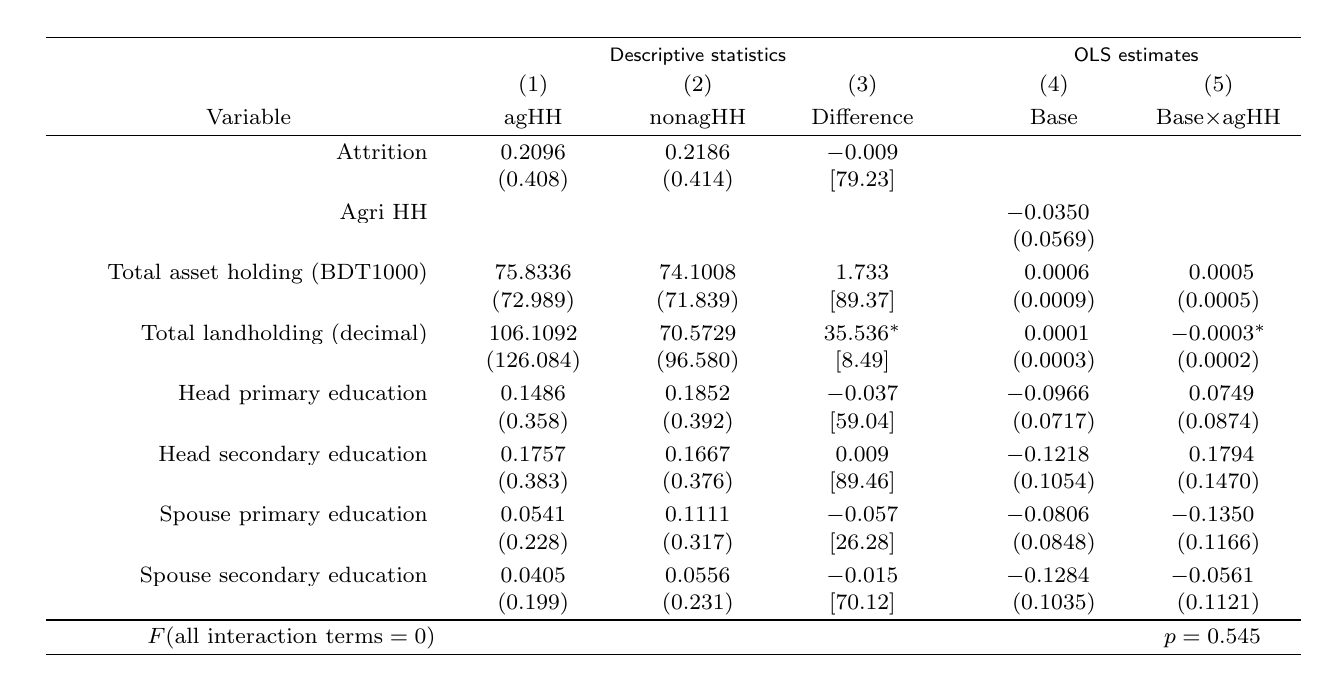
\begin{tikzpicture}
\node (tbl) {
\setlength{\tabcolsep}{2pt}
\begin{tabular}{
>{\footnotesize\hfil$}p{5cm}<{$}
>{\footnotesize\hfil$}p{1.95cm}<{$}
>{\footnotesize\hfil$}p{1.95cm}<{$}
>{\footnotesize\hfil$}p{1.95cm}<{$}
>{$}p{0.2cm}<{$}
>{\footnotesize\hfil$}p{1.95cm}<{$}
>{\footnotesize\hfil$}p{1.95cm}<{$}
>{\footnotesize\hfil$}p{1.95cm}<{$}}
\rowcolor{white}\hline
\makebox[4.75cm]{\scriptsize\hfil}&\multicolumn{3}{c}{\makebox[5.85cm]{\scriptsize \textsf{Descriptive statistics}}}&&\multicolumn{2}{c}{\makebox[3.9cm]{\scriptsize \textsf{OLS estimates}}} \\[-.25ex]
\cline{2-4} \cline{6-7}\rowcolor{white}
 & (1) & (2) & (3) & & (4) & (5)\\
\makebox[4cm]{\cellcolor{white}Variable} & \makebox[1.95cm]{\cellcolor{white}agHH} & \makebox[1.95cm]{\cellcolor{white}nonagHH} & \makebox[1.95cm]{\cellcolor{white}Difference} & \makebox[0.2cm]{\cellcolor{white}} & \makebox[1.95cm]{\cellcolor{white}Base} & \makebox[1.95cm]{\cellcolor{white}Base$\times$agHH}\\
\hline
\makebox[4.75cm]{\hfill Attrition } & 0.2096 & 0.2186 & -0.009 &  &  & \\[-.5ex]
\makebox[4.75cm]{\hfill  } & (0.408) & (0.414) & [79.23] &  &  & \\\rowcolor{white}
\makebox[4.75cm]{\hfill Agri HH } &  &  &  &  & -0.0350\phantom{^{*}} & \\[-.5ex]\rowcolor{white}
\makebox[4.75cm]{\hfill  } &  &  &  &  & (0.0569) & \\
\makebox[4.75cm]{\hfill Total asset holding (BDT1000) } & 75.8336 & 74.1008 & 1.733 &  & \phantom{-}0.0006\phantom{^{*}} & \phantom{-}0.0005\phantom{^{*}}\\[-.5ex]
\makebox[4.75cm]{\hfill  } & (72.989) & (71.839) & [89.37] &  & (0.0009) & (0.0005)\\\rowcolor{white}
\makebox[4.75cm]{\hfill Total landholding (decimal) } & 106.1092 & 70.5729 & 35.536^{*} &  & \phantom{-}0.0001\phantom{^{*}} & -0.0003^{*}\\[-.5ex]\rowcolor{white}
\makebox[4.75cm]{\hfill  } & (126.084) & (96.580) & [8.49] &  & (0.0003) & (0.0002)\\
\makebox[4.75cm]{\hfill Head primary education } & 0.1486 & 0.1852 & -0.037 &  & -0.0966\phantom{^{*}} & \phantom{-}0.0749\phantom{^{*}}\\[-.5ex]
\makebox[4.75cm]{\hfill  } & (0.358) & (0.392) & [59.04] &  & (0.0717) & (0.0874)\\\rowcolor{white}
\makebox[4.75cm]{\hfill Head secondary education } & 0.1757 & 0.1667 & 0.009 &  & -0.1218\phantom{^{*}} & \phantom{-}0.1794\phantom{^{*}}\\[-.5ex]\rowcolor{white}
\makebox[4.75cm]{\hfill  } & (0.383) & (0.376) & [89.46] &  & (0.1054) & (0.1470)\\
\makebox[4.75cm]{\hfill Spouse primary education } & 0.0541 & 0.1111 & -0.057 &  & -0.0806\phantom{^{*}} & -0.1350\phantom{^{*}}\\[-.5ex]
\makebox[4.75cm]{\hfill  } & (0.228) & (0.317) & [26.28] &  & (0.0848) & (0.1166)\\\rowcolor{white}
\makebox[4.75cm]{\hfill Spouse secondary education } & 0.0405 & 0.0556 & -0.015 &  & -0.1284\phantom{^{*}} & -0.0561\phantom{^{*}}\\[-.5ex]\rowcolor{white}
\makebox[4.75cm]{\hfill  } & (0.199) & (0.231) & [70.12] &  & (0.1035) & (0.1121)\\
\hline
\makebox[4.75cm]{\hfill $F (\mbox{all interaction terms}=0)$} &  &  & &  &  & p=0.545\phantom{^{*}}\\\hline
\end{tabular}
};
\end{tikzpicture}\\
\renewcommand{\arraystretch}{.8}
\setlength{\tabcolsep}{1pt}
\hfil\begin{tabular}{>{\hfill\scriptsize}p{1cm}<{}>{\hfill\scriptsize}p{.25cm}<{}>{\scriptsize}p{13.75cm}<{\hfill}}
Source:& \multicolumn{2}{l}{\scriptsize Compiled from IFPRI data.}\\
Notes: & 1. & Attrition is true if a household is missing in round 2. All covariates are of round 1.\\
& 2. & \textsf{Descriptive statistics} panel shows attriter's characteristics. The top rows show the means, and the bottom rows show the standard errors in columns (1) and (2), respectively. In column (3), the top rows show mean differences, and the bottom rows show associated $p$ values of mean differences in percentage. \textsf{OLS estimation} panel shows results from a linear probability model of attrition on baseline variables $\bfx_{i}$ and their interaction with the agricultural household dummy $r_{i}$: $y_{i}=\bfbeta'\bfx_{i}+\bfgamma'r_{i}\bfx_{i}+e_{i}$. For each covariates, the top rows show point estimates, and the bottom rows show standard errors. Estimates of non-agricultural HHs $\bfbeta$ are shown in column (4), and interaction terms $\bfgamma$ of each variable with agricultural HH are shown in column (5). Number of observations for LPM is $570$, $\bar{R}=0.058$. Standard errors are shown in parentheses, which are clustered at the Thana level with a Satterthwaite correction for a small number of clusters. For column (3), $p$ values of the null of zero difference are shown in square brackets. $*$ indicates a $p$ value between 5\% and 10\%. 
\end{tabular}
\end{minipage}
\end{table}

Table \ref{tab destat zEm1999} summarizes the data used in the regressions. Based on the age cut-off of 10 years and older in the 1999 survey, we have 626 observations. In our sample, approximately 61 percent of households were categorized as agricultural households. Alternative agricultural household definitions give similar summary statistics, which explains the small difference in estimation. The household head's highest level of education is mostly secondary, 28\%, and the primary level comprises 15.5\% of our sample. Spousal education is similar for the primary level, 17\%, but relatively low for the secondary level, 16.6\%. The mean per member landholding is 0.168 acre. Median per member non-land assets are about 11,000 BDT (110 USD), and about 14,000 BDT (140 USD) at the 75th percentile. These non-land asset values indicate that our sample primarily comprises poor rural households.

For the placebo sample, we took 10 to 18 years in 2002 (2002 cohort) to compare with the main data. \textsc{Table \ref{tab destat zEp2002}} presents a summary of the data used in the placebo regressions. Based on the age cutoff of 10 years and older in the 2002 survey, there are 812 observations in the placebo sample. In our placebo sample, we have about 60\% agricultural households, which is quite similar to the main sample. Other summary statistics reported in Table \ref{tab destat zEm1999} show close similarity with Table \ref{tab destat zEp2002}. This demonstrates the validity of a placebo sample, at least observational. The only notable observable difference between these two samples, however, is the declining enrollment rate, which is about 11 percentage points lower than the 1999 average.

\begin{minipage}[t]{.8\paperwidth}
\hfil\textsc{\normalsize Table \refstepcounter{table}\thetable: \begin{minipage}[t]{.6\paperwidth}
Descriptive statistics of main estimation,\\ 10-18 years old, direct offspring\setlength{\baselineskip}{8pt}
\end{minipage}
\label{tab destat zEm1999}}\\
\setlength{\tabcolsep}{1pt}
\renewcommand{\arraystretch}{.6}
%\hfil\begin{tabular}{>{\scriptsize}p{5cm}<{\hfill}>{\hfill\scriptsize$}p{0.75cm}<{$}>{\hfill\scriptsize$}p{0.75cm}<{$}>{\hfill\scriptsize$}p{0.75cm}<{$}>{\hfill\scriptsize$}p{0.75cm}<{$}>{\hfill\scriptsize$}p{0.75cm}<{$}>{\hfill\scriptsize$}p{1cm}<{$}>{\hfill\scriptsize$}p{0.75cm}<{$}>{\hfill\scriptsize$}p{0.75cm}<{$}>{\hfill\scriptsize$}p{0.75cm}<{$}>{\hfill\scriptsize$}p{0.75cm}<{$}}
\makebox[5cm]{covariates} & \makebox[0.75cm]{min} & \makebox[0.75cm]{25\%} & \makebox[0.75cm]{median} & \makebox[0.75cm]{75\%} & \makebox[0.75cm]{max} & \makebox[1cm]{mean} & \makebox[0.75cm]{std} & \makebox[0.75cm]{0s} & \makebox[0.75cm]{NAs} & \makebox[0.75cm]{n}\\
Enrolled & 0 & 0 & 1 & 1 & 1 & 0.738 & 0.440 & 164 & 0 & 626\\
Agricultural household (combined) & 0 & 0 & 1 & 1 & 1 & 0.613 & 0.487 & 242 & 0 & 626\\
Agricultural household (head definition) & 0 & 0 & 1 & 1 & 1 & 0.553 & 0.498 & 280 & 0 & 626\\
Agricultural household (income definition) & 0 & 0 & 1 & 1 & 1 & 0.575 & 0.495 & 266 & 0 & 626\\
Agricultural household (occupation definition) & 0 & 0 & 1 & 1 & 1 & 0.543 & 0.499 & 286 & 0 & 626\\
Membership to stipend program & 0 & 0 & 0 & 1 & 1 & 0.315 & 0.465 & 429 & 0 & 626\\
Membership to non-stipend program & 0 & 0 & 0 & 1 & 1 & 0.425 & 0.495 & 360 & 0 & 626\\
Sex & 0 & 0 & 1 & 1 & 1 & 0.511 & 0.500 & 306 & 0 & 626\\
Head sex (female = 1) & 0 & 0 & 0 & 0 & 1 & 0.128 & 0.334 & 546 & 0 & 626\\
Non-Muslim & 0 & 0 & 0 & 0 & 1 & 0.123 & 0.329 & 549 & 0 & 626\\
Flooded & 0 & 0 & 1 & 1 & 1 & 0.623 & 0.485 & 236 & 0 & 626\\
Structured toilet & 0 & 0 & 0 & 1 & 1 & 0.294 & 0.456 & 442 & 0 & 626\\
\hspace{.5em}Own piped water & 0 & 0 & 0 & 1 & 1 & 0.380 & 0.486 & 388 & 0 & 626\\
head primary & 0 & 0 & 0 & 0 & 1 & 0.155 & 0.362 & 529 & 0 & 626\\
head secondary & 0 & 0 & 0 & 1 & 1 & 0.284 & 0.451 & 448 & 0 & 626\\
head spouse primary & 0 & 0 & 0 & 0 & 1 & 0.171 & 0.377 & 519 & 0 & 626\\
head spouse secondary & 0 & 0 & 0 & 0 & 1 & 0.166 & 0.372 & 522 & 0 & 626\\
age & 10 & 11 & 13 & 15 & 18 & 12.986 & 2.351 & 0 & 0 & 626\\
yield (thana) & 0.607 & 0.647 & 0.823 & 0.906 & 0.928 & 0.786 & 0.110 & 0 & 0 & 626\\
Number of older female siblings & 0 & 0 & 0 & 1 & 4 & 0.390 & 0.670 & 434 & 0 & 626\\
Number of older male siblings & 0 & 0 & 0 & 1 & 5 & 0.577 & 0.844 & 376 & 0 & 626\\
per member land holding (decimal, in 1999) & 0 & 0.019 & 0.069 & 0.196 & 3.215 & 0.167 & 0.287 & 2 & 0 & 626\\
per member nonland asset (1000 Tk, in 1999) & 0.373 & 3.918 & 7.062 & 13.623 & 205 & 11.209 & 14.515 & 0 & 0 & 626\\
\end{tabular}
\\

\renewcommand{\arraystretch}{.55}
\setlength{\tabcolsep}{1pt}
\begin{tabular}{>{\hfill\scriptsize}p{1cm}<{}>{\hfill\scriptsize}p{.25cm}<{}>{\scriptsize}p{.6\paperwidth}<{\hfill}}
Source:& \multicolumn{2}{l}{\scriptsize Compiled from IFPRI data.}\\
Notes: & 1. & All information is of year 1999.\\
& 2. & Agricultural households are defined as at least one adult member claiming that the main income source is agriculture or occupation is agriculture. Program membership is one if holding a membership to anti-poverty programs. STD represents Standard deviation.\setlength{\baselineskip}{6pt}
\end{tabular}
\end{minipage}

\begin{minipage}[t]{.8\paperwidth}
\hfil\textsc{\normalsize Table \refstepcounter{table}\thetable: \begin{minipage}[t]{.6\paperwidth}
Descriptive statistics of placebo estimation,\\ 10-18 years old in 2002, direct offspring
\setlength{\baselineskip}{8pt}
\end{minipage}
\label{tab destat zEp2002}}\\
\setlength{\tabcolsep}{1pt}
\renewcommand{\arraystretch}{.6}
%\hfil\begin{tabular}{>{\scriptsize\hfill}p{5.75cm}<{}>{\hfill\scriptsize$}p{0.85cm}<{$}>{\hfill\scriptsize$}p{0.85cm}<{$}>{\hfill\scriptsize$}p{0.85cm}<{$}>{\hfill\scriptsize$}p{0.85cm}<{$}>{\hfill\scriptsize$}p{0.85cm}<{$}>{\hfill\scriptsize$}p{1cm}<{$}>{\hfill\scriptsize$}p{0.85cm}<{$}>{\hfill\scriptsize$}p{0.85cm}<{$}>{\hfill\scriptsize$}p{0.85cm}<{$}>{\hfill\scriptsize$}p{0.85cm}<{$}}
\makebox[5.75cm]{covariates} & \makebox[0.85cm]{min} & \makebox[0.85cm]{25\%} & \makebox[0.85cm]{median} & \makebox[0.85cm]{75\%} & \makebox[0.85cm]{max} & \makebox[1cm]{mean} & \makebox[0.85cm]{std} & \makebox[0.85cm]{0s} & \makebox[0.85cm]{NAs} & \makebox[0.85cm]{n}\\
\hline
Enrolled & 0 & 0 & 1 & 1 & 1 & 0.631 & 0.483 & 300 & 0 & 812\\
Agricultural household (combined definition) & 0 & 0 & 1 & 1 & 1 & 0.606 & 0.489 & 320 & 0 & 812\\
Agricultural household (head definition) & 0 & 0 & 1 & 1 & 1 & 0.542 & 0.499 & 372 & 0 & 812\\
Agricultural household (income definition) & 0 & 0 & 1 & 1 & 1 & 0.562 & 0.496 & 356 & 0 & 812\\
Agricultural household (occupation definition) & 0 & 0 & 1 & 1 & 1 & 0.537 & 0.499 & 376 & 0 & 812\\
Membership to stipend program & 0 & 0 & 0 & 1 & 1 & 0.273 & 0.446 & 590 & 0 & 812\\
Membership to non-stipend program & 0 & 0 & 0 & 0 & 1 & 0.002 & 0.050 & 810 & 0 & 812\\
Sex (female = 1) & 0 & 0 & 1 & 1 & 1 & 0.525 & 0.500 & 386 & 0 & 812\\
Head sex (female = 1) & 0 & 0 & 0 & 0 & 1 & 0.116 & 0.320 & 718 & 0 & 812\\
Flooded & 0 & 0 & 1 & 1 & 1 & 0.626 & 0.484 & 304 & 0 & 812\\
Structured toilet & 0 & 0 & 0 & 1 & 1 & 0.282 & 0.450 & 583 & 0 & 812\\
\hspace{.5em}Own piped water & 0 & 0 & 0 & 1 & 1 & 0.376 & 0.485 & 507 & 0 & 812\\
Head education: primary & 0 & 0 & 0 & 0 & 1 & 0.159 & 0.366 & 683 & 0 & 812\\
Head education: secondary & 0 & 0 & 0 & 1 & 1 & 0.281 & 0.450 & 584 & 0 & 812\\
Head's spouse education: primary & 0 & 0 & 0 & 0 & 1 & 0.177 & 0.382 & 668 & 0 & 812\\
Head's spouse education: secondary & 0 & 0 & 0 & 0 & 1 & 0.166 & 0.373 & 677 & 0 & 812\\
Age & 10 & 12 & 13 & 16 & 18 & 13.631 & 2.470 & 0 & 0 & 812\\
Yield (thana) & 0.69 & 0.743 & 0.838 & 0.984 & 1.036 & 0.848 & 0.117 & 0 & 0 & 812\\
Number of older female siblings & 0 & 0 & 0 & 1 & 4 & 0.560 & 0.793 & 477 & 0 & 812\\
Number of older male siblings & 0 & 0 & 0 & 1 & 5 & 0.659 & 0.882 & 447 & 0 & 812\\
Per member land holding (decimal, in 1999) & 0 & 0.017 & 0.063 & 0.179 & 3.215 & 0.160 & 0.289 & 2 & 0 & 812\\
Per member nonland asset (1000 Tk, in 1999) & 0.369 & 3.537 & 6.963 & 13.143 & 205 & 10.994 & 14.995 & 0 & 0 & 812\\
\end{tabular}
\\

\renewcommand{\arraystretch}{.55}
\setlength{\tabcolsep}{1pt}
\begin{tabular}{>{\hfill\scriptsize}p{1cm}<{}>{\hfill\scriptsize}p{.25cm}<{}>{\scriptsize}p{.6\paperwidth}<{\hfill}}
Source:& \multicolumn{2}{l}{\scriptsize Compiled from IFPRI data.}\\
Notes: & 1. & All information is of year 2002 except for \textsf{Enrolled, Yield, Temperature, Rainfall, Program membership}.\\
& 2. & Agricultural households are defined as at least one adult member claiming that the main income source is agriculture or occupation is agriculture. Program membership is one of holding a membership to anti-poverty programs. STD represents Standard deviation. \setlength{\baselineskip}{6pt}
\end{tabular}
\end{minipage}

\pagebreak


To assess relative impoverishment, we tabulated agriculture and non-agricultural households based on household consumption information in Table \ref{agpc4}. The consumption quartiles are derived based on per-member consumption information in the household. We noticed a higher consumption quartile for non-agricultural households compared to Agricultural households.

The IFPRI panel data set reports reasons for dropping out of school (\textsc{\small Table \ref{reasons}}). We notice dropout rates are higher for lower consumption quartiles, and their reasons for dropping out primarily include financial difficulties, which is also true for irregular students. Upper-quartile individuals cite non-financial reasons such as marriage as the reason for drop-out. We also summarize the reported reasons for school dropout by household type in {\textsc{\small Table \ref{reasons2}}: agricultural or non-agricultural households. Our table indicates that agricultural households cite financial reasons more frequently than non-agricultural ones as the main reason for dropping out and school irregularity. 

\begin{table}
\caption{Tabulation of Agricultural vs. Non-Agriculture household Consumption Quartiles}
\label{agpc4}
\begin{center}
{
\resizebox{11.5cm}{!}{
\begin{tabular}{lcccccc}
\hline
Quartiles & 1     & 2         & 3          & 4        & `NA's         &       N    \\
\hline
Agricultural households  & 25.8 &      27.27 &      26.54 &      19.66 & 0.74 &   407 \\
Non-agricultural households & 23.27 &  24.36 &  18.55 &   33.82 &   0 &        275 \\
\hline
\hline
\multicolumn{7}{p{12cm}}{{\footnotesize Notes: Consumption quartiles are based on households.}}
\end{tabular}}}
\end{center}
\end{table}

\begin{table}[bp]
\caption{Reported Reasons for Stop Going to School by Consumption Quartiles and by Household Type}
\label{reasons}
\begin{center}
{
\resizebox{15cm}{!}{
\begin{tabular}{cccccccccc}
\hline
Quartile & Group & \scriptsize{Financial} & \scriptsize {Not accepted} & \scriptsize {School environment} & \scriptsize {Marriage} & \scriptsize {Distance} & \scriptsize {Sickness} & NA & Total                        \\
\hline
1 & Irregular 1999 &  0.52 &  0.03 &  0.2 & 0    & 0.06 & 0.02 & 0.17 & 65 \\
1 & Irregular 2002 &  0.54 &  0.01 & 0.01 & 0.01 & 0.01 &    0 & 0.43 & 115 \\
1 & Drop outs 2002 &  0.62 &     0 & 0.02 & 0.02 &    0 &    0 & 0.34 &  58 \\
\hline
2 & Irregular 1999 &  0.48 &    0 &    0.23 &     0 &   0.14 &    0  &    0.14 &   56 \\
2 & Irregular 2002 &  0.37 &    0 &    0.06 &  0.01 &   0.02 &  0.01 &    0.52 &   81 \\
2 & Drop outs 2002 &  0.41 &    0 &    0.08 &     0 &   0.03 &     0 &    0.49 &   37 \\
\hline
3 & Irregular 1999 &   0.44 &      0 &    0.26 &     0 &     0.18 &    0.09 &    0.03 &   34 \\
3 & Irregular 2002 &   0.28 &      0 &       0 &  0.05 &     0.03 &    0.03 &    0.61 &   64 \\
3 & Drop outs 2002 &   0.26 &      0 &       0 &  0.05 &     0.03 &    0.03 &    0.63 &   38 \\
\hline
4 & Irregular 1999 &   0.45 &   0.05 &   0.18 &      0 &    0.05 &    0.05 &    0.23 &    22 \\
4 & Irregular 2002 &    0.1 &   0.01 &   0.03 &   0.03 &    0.01 &    0.03 &    0.79 &    73 \\
4 & Drop outs 2002 &   0.11 &   0.02 &   0.02 &   0.04 &       0 &    0.04 &    0.78 &    54 \\
\hline\\
\hline
\multicolumn{10}{p{21cm}}{{\footnotesize Notes: Numbers are all ratios except totals. ``Agri HH'' indicates agricultural households. See main text for definition of agricultural households. Irregulars are individuals who were not enrolled in the respective period. Dropouts are individuals who were enrolled in 1999 but not in 2002..}}
\end{tabular}}}
\end{center}
\end{table}



\begin{table}[bp]
\caption{Reasons for Not Going to School, Agricultural vs. Non-Agriculture household}
\label{reasons2}
\begin{center}
{
\resizebox{14.5cm}{!}{
\begin{tabular}{cccccccccc}
\hline
{\bf HH Type} & {\bf Group} & {\bf Financial} & {\bf Not accepted} & {\bf School Environment} & {\bf Marriage} & {\bf Distance} & {\bf Sickness} &   {\bf NA} & {\bf Total} \\
\hline
Ag      & Irregular 1999 &  0.55 &  0.03 &  0.21 &    0 &  0.06 &   0.05 &   0.11 &   66 \\
Ag      & Irregular 2002 &  0.38 &     0 &  0.01 & 0.01 &  0.01 &   0.02 &   0.57 &  120 \\
Ag      & drop outs 2002 &  0.46 &     0 &  0.01 &    0 &  0.01 &   0.01 &    0.5 &   70 \\
\hline
Non-ag  & Irregular 1999 &  0.46 &  0.01 &  0.22 &    0 &  0.13 &   0.02 &   0.16 &  112 \\
Non-ag  & Irregular 2002 &  0.33 &  0.01 &  0.03 & 0.03 &  0.02 &   0.01 &   0.56 &  214 \\
Non-ag  & drop outs 2002 &   0.3 &  0.01 &  0.03 & 0.04 &  0.01 &   0.02 &   0.59 &  117 \\
\hline
\hline
\multicolumn{10}{p{22cm}}{{\footnotesize Notes: Numbers are all ratios except totals. ``Agri HH'' indicates agricultural households. See the main text for the definition of agricultural households. Irregulars are individuals who were not enrolled in the respective period. Dropouts are individuals who were enrolled in 1999 but not in 2002..}}
\end{tabular}}}
\end{center}
\end{table}



\begin{figure}[h!]
%\hspace{-2em}\begin{minipage}[t]{13cm}
\hfil\textsc{\footnotesize Figure \refstepcounter{figure}\thefigure: Enrollment rates by age and HH type, 1999, 5 years and older\label{ERbyAge rawdata}}\\
\hfil 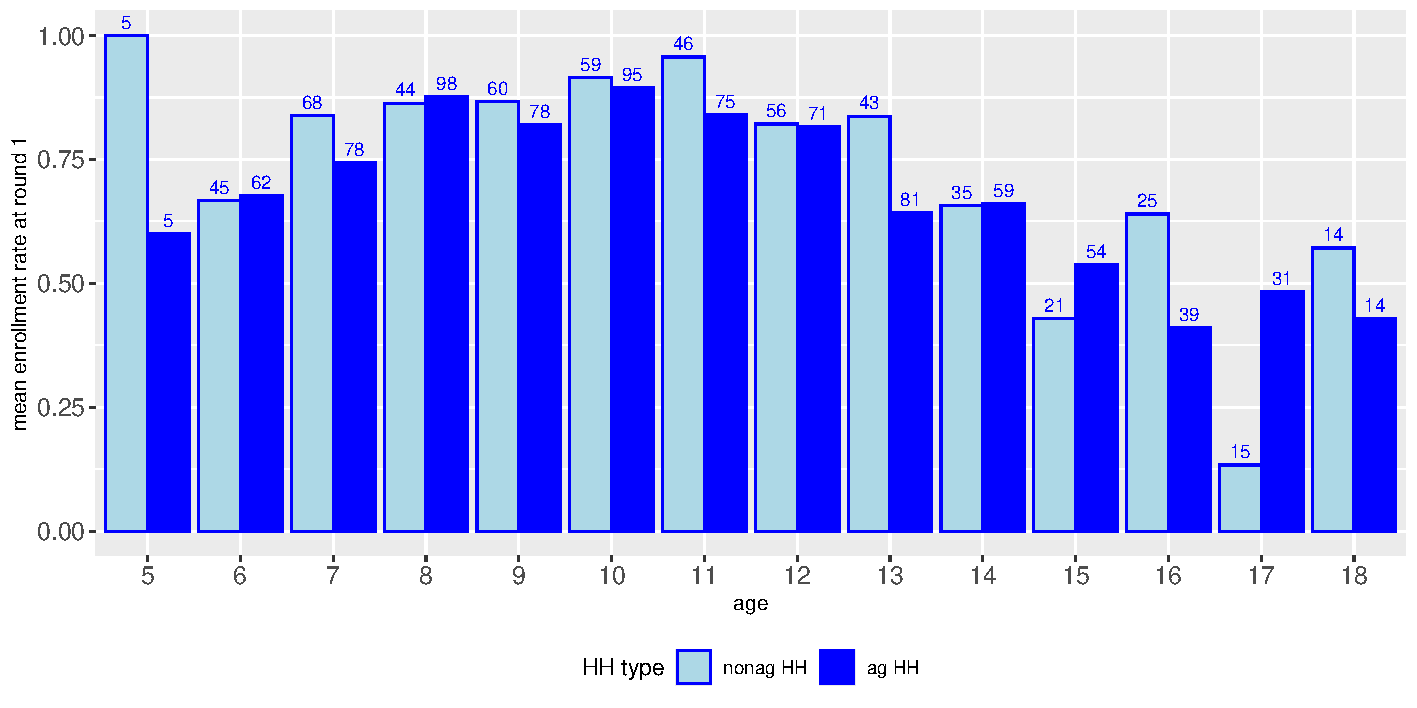
\includegraphics[width=.7\paperwidth]{Figures/AgewiseRawEnrollmentRates.pdf}\\
\renewcommand{\arraystretch}{1}
\hfil\begin{tabular}{>{\hfill\scriptsize}p{1cm}<{}>{\scriptsize}p{12cm}<{\hfill}}
Source:& Compiled from IFPRI data. All households, including attrited households, are used.\\[-1ex]
Notes:& Ages are of round 1. Numbers displayed above the bar are cell sample size. \\[-1ex]
\end{tabular}
%\end{minipage}
\end{figure}

\begin{figure}[h!]
%\hspace{-2em}\begin{minipage}[t]{13cm}
\hfil\textsc{\footnotesize Figure \refstepcounter{figure}\thefigure: Age starting the primary school by year and HH type, reported in 2000\label{AgeAtClass1byAge rawdata}}\\
\hfil 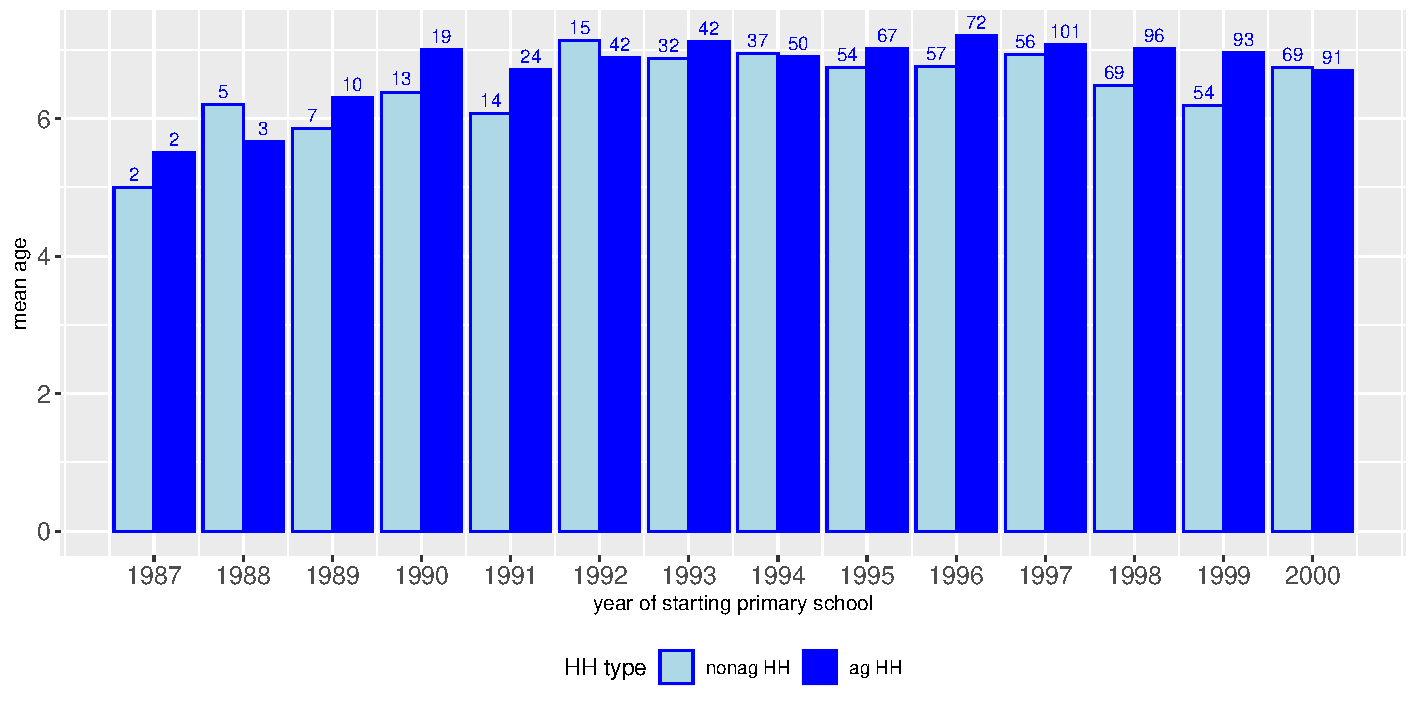
\includegraphics[width=.7\paperwidth]{Figures/AgeAtClass1Enrollment.pdf}\\
\renewcommand{\arraystretch}{1}
\hfil\begin{tabular}{>{\hfill\scriptsize}p{1cm}<{}>{\scriptsize}p{12cm}<{\hfill}}
Source:& Compiled from IFPRI data. All households, including attrited households, are used.\\[-1ex]
Notes:&: The Numbers displayed above the bar are cell sample size. \\[-1ex]
\end{tabular}
%\end{minipage}
\end{figure}

\textsc{\footnotesize Figure \ref{ERbyAge rawdata}} shows mean enrollment rates by age. Ages under primary and secondary schooling have less than 100\% enrollment rates. Age 5, one year before primary schooling begins, reports nonzero enrollment rates. These show that ``compulsory schooling'' is not enforced strictly. 

\textsc{\footnotesize Figure \ref{AgeAtClass1byAge rawdata}} shows the mean age of starting class 1 for each calendar year. Most years report the mean starting age older than six years old. This also shows that ``compulsory schooling'' is not enforced strictly. Agricultural households tend to start school later in age than non-agricultural households. This may partly explain why Agricultural households's enrollment rates are higher at some of the later ages. 




\clearpage


\section{Additional figures and tables\label{app_a4}}


\subsection{Figures}

%\hspace{-2em}\begin{minipage}[t]{13cm}
\hfil\textsc{\footnotesize Figure \refstepcounter{figure}\thefigure: Impacts by main/placebo by gender and by agricutural household definition\label{App_MainVsPlaceboPlotsByAgdefByGender}}\\
\hfil 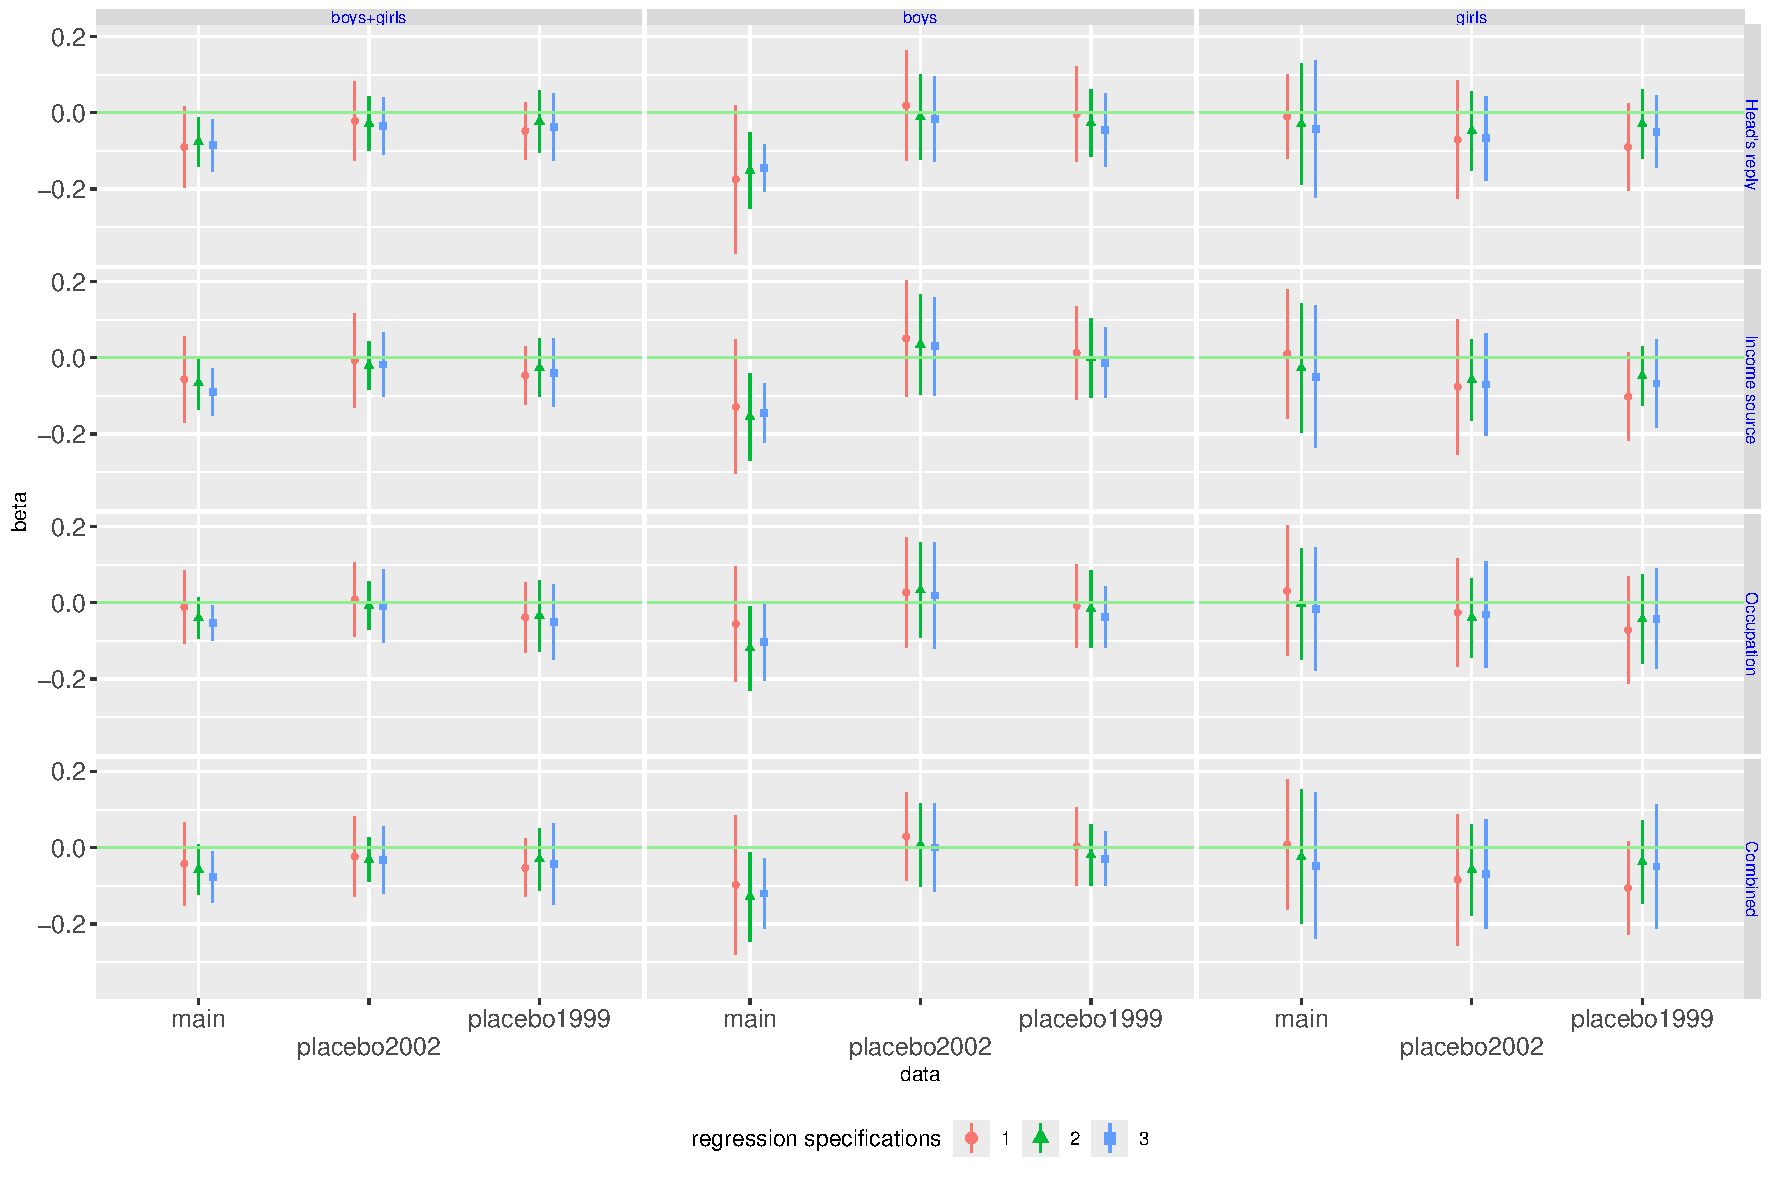
\includegraphics[width=.7\paperwidth]{Figures/App_MainVsPlaceboPlotsByAgdefByGender.pdf}\\
\renewcommand{\arraystretch}{1}
\hfil\begin{tabular}{>{\hfill\scriptsize}p{1cm}<{}>{\hfill\scriptsize}p{.5cm}<{}>{\scriptsize}p{12cm}<{\hfill}}
Source: & \multicolumn{2}{l}{\scriptsize Compiled from IFPRI data.} \\[-1ex]
Notes:& 1. & Each row shows the estimates under different agricultural household definitions. Income source base, head's reply base, occupation base, and all combined (with ``or'' operations). Each column shows estimates using gender subsamples and full sample. The coefficients are for agricultural HH $\times$ year 2002 for main data and agricultural HH $\times$ year 2006 for placebo 2002 and placebo 1999 data.\setlength{\baselineskip}{10pt}\\[-1ex]
& 2. & Specifications 1 - 3 correspond to the same specifications in \textsc{Table \ref{base10}}. \\[-1ex]
& 3. & Error bars are 95\% confidence intervals using standard errors clustered at thana level with a Satterthwaite correction for small number of clusters.\setlength{\baselineskip}{10pt}
\end{tabular}
%\end{minipage}


\begin{figure}
%\hspace{-2em}\begin{minipage}[t]{13cm}
\hfil\textsc{\footnotesize Figure \refstepcounter{figure}\thefigure: Impacts by age lowerbound, 1999-2002\label{GenderByAgeLBImpacts}}\\
\hfil 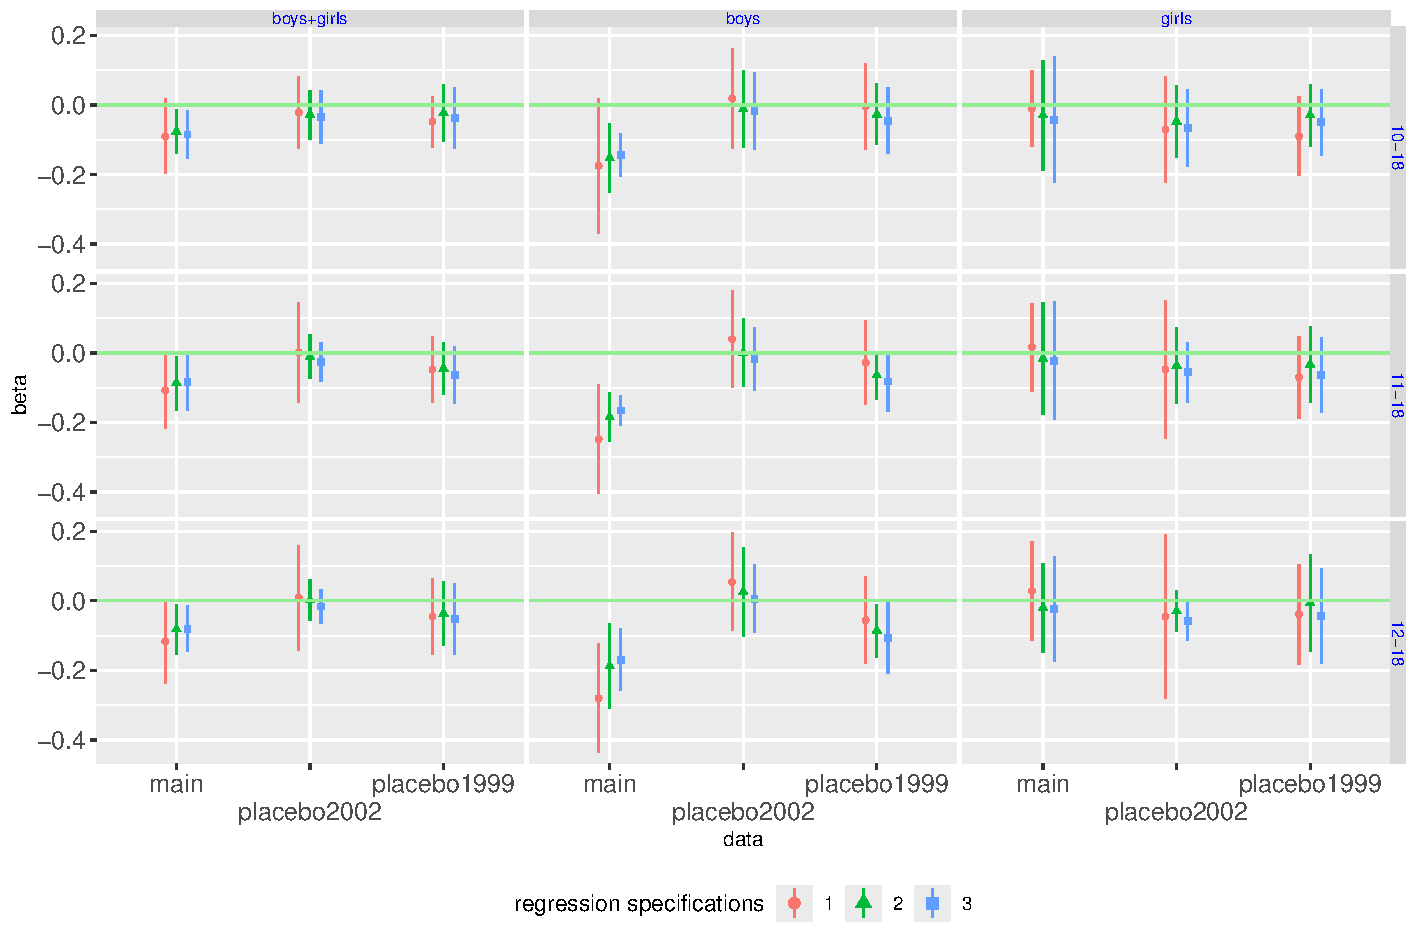
\includegraphics[width=.7\paperwidth]{Figures/App_MainVsPlaceboPlotsByAgeLBByGender.pdf}\\
\renewcommand{\arraystretch}{1}
\hfil\begin{tabular}{>{\hfill\scriptsize}p{1cm}<{}>{\hfill\scriptsize}p{.5cm}<{}>{\scriptsize}p{11cm}<{\hfill}}
Source: & \multicolumn{2}{l}{\scriptsize Compiled from IFPRI data.} \\[-1ex]
Notes:& 1. & 10-18, 11-18, 12-18 indicate age range of each sample. The coefficients are dummies for agri-HH $\times$ year 2002.\\[-1ex]
& 2. & Specifications 1 - 3 correspond to the same specifications in \textsc{Table \ref{base10}}. \\[-1ex]
& 3. & Error bars are 95\% confidence intervals using standard errors clustered at thana level with a Satterthwaite correction for small number of clusters.
\end{tabular}
%\end{minipage}
\end{figure}

\begin{figure}
%\hspace{-2em}\begin{minipage}[t]{13cm}
\hfil\textsc{\footnotesize Figure \refstepcounter{figure}\thefigure: Other outcomes by gender, 1999-2002\label{NumGradesDaysAbsentPlots}}\\
\hfil 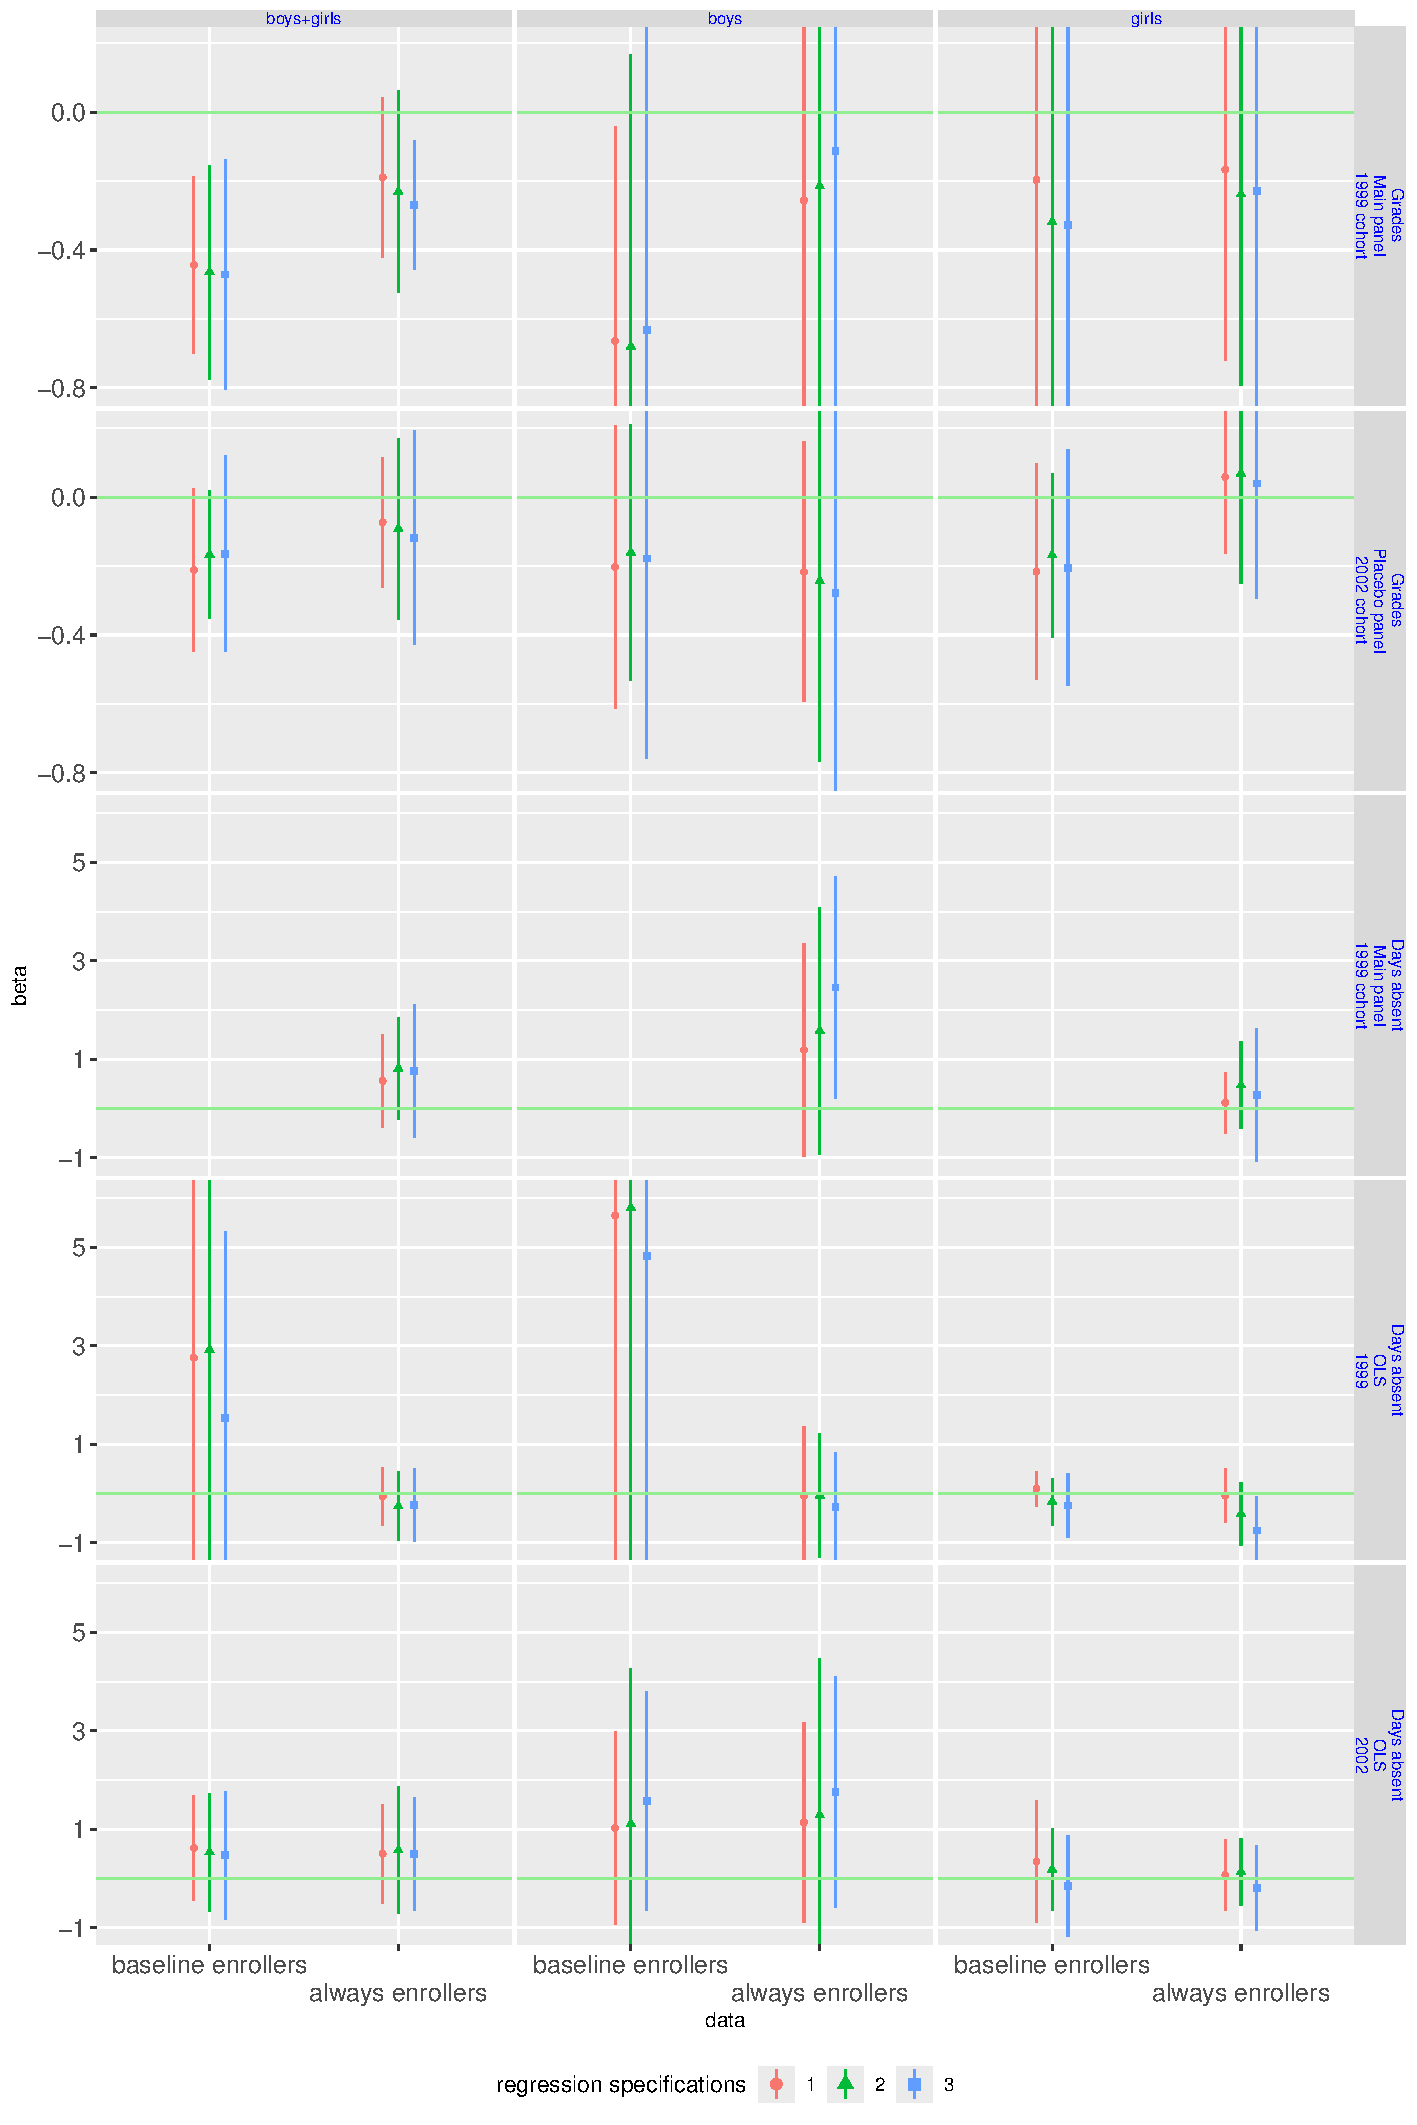
\includegraphics[width=.7\paperwidth]{Figures/App_NumGradesDaysAbsentPlotsByGender.pdf}\\
\renewcommand{\arraystretch}{1}
\hfil\begin{tabular}{>{\hfill\scriptsize}p{1cm}<{}>{\hfill\scriptsize}p{.5cm}<{}>{\scriptsize}p{11cm}<{\hfill}}
Source: & \multicolumn{2}{l}{\scriptsize Compiled from IFPRI data.} \\[-1ex]
Notes:& 1. & Grades: Number of grades, Days: Days absent. Rows are for number of grades impacts, number of grades placebo impacts, and days absent impacts.  Panel of ``Days, placebo'' is not shown because there is no placebo test for it. Columns are for boys subsample, girls subsample, and full sample. \textsf{complete}: Complete panel sample, \textsf{incomplete}: Incomplete panel sample, \textsf{cross section 1999}: 1999 cross section estimate of incomplete panel sample, \textsf{cross section 2002}: 2002 cross section estimate of incomplete panel sample. The coefficients are for agricultural HH $\times$ year 2002 for ``Grades'', ``Days absent'' rows and agricultural HH $\times$ year 2006 for ``Grades, placebo'' row.\\[-1ex]
& 2. & Specifications 1 - 3 correspond to the same specifications in \textsc{Table \ref{base10}}. \\[-1ex]
& 3. & Error bars are 95\% confidence intervals using standard errors clustered at thana level with a Satterthwaite correction for small number of clusters.
\end{tabular}
%\end{minipage}
\end{figure}

\clearpage
\subsection{Tables}


\begin{figure}[ht!]
\centering
\includegraphics[width = 11.5cm, height = 15cm]{Figures/Secondary School-Holiday-List-2019.jpg}\\
\caption{Government School Calendar in Bangladesh (2019).\protect\footnotemark}
\label{school_calander_2019}
\end{figure}

\footnotetext{Above is the Ministry of Education (MoE) Bangladesh provided examination and annual holiday calendar for the secondary and higher secondary schools (in Bangla). The bottom table of this notice contains the exam calendar, which instructed all the schools to hold annual exams from November 27 to December 11.}

\pagebreak

\begin{table}
\hfil\textsc{\footnotesize Table \refstepcounter{table}\thetable: Main results by gender and by agricultural household definitions\label{MainGenderByAgdefResults}}\\
\setlength{\tabcolsep}{1pt}
\renewcommand{\arraystretch}{.75}
\hspace{-1.0cm}\begin{tabular}{>{\scriptsize}p{3.25cm}<{\hfill}>{\hfil\scriptsize$}p{1.5cm}<{$}>{\hfil\scriptsize$}p{1.5cm}<{$}>{\hfil\scriptsize$}p{1.5cm}<{$}>{$}p{0.1cm}<{$}>{\hfil\scriptsize$}p{1.5cm}<{$}>{\hfil\scriptsize$}p{1.5cm}<{$}>{\hfil\scriptsize$}p{1.5cm}<{$}>{$}p{0.1cm}<{$}>{\hfil\scriptsize$}p{1.5cm}<{$}>{\hfil\scriptsize$}p{1.5cm}<{$}>{\hfil\scriptsize$}p{1.5cm}<{$}}
\hline
\makebox[3.25cm]{\scriptsize\hfil }&\multicolumn{3}{c}{\makebox[4.5cm]{\scriptsize \textsf{Boys+girls}}}&&\multicolumn{3}{c}{\makebox[4.5cm]{\scriptsize \textsf{Boys}}}&&\multicolumn{3}{c}{\makebox[3.1cm]{\scriptsize \textsf{Girls}}} \\[-.5ex]
\cline{2-4} \cline{6-8} \cline{10-12} \\[-1ex]
&\textsf{Spec 1} & \textsf{Spec 2} & \textsf{Spec 3}&&\textsf{Spec 1} & \textsf{Spec 2} & \textsf{Spec 3}&&\textsf{Spec 1} & \textsf{Spec 2} & \textsf{Spec 3}\\
&\multicolumn{11}{l}{}\\
A. AgHH: Head's reply & (1)&(2)&(3)&&(4)&(5)&(6)&&(7)&(8)&(9) \\
Agricultural HH * year 2002 & -0.0897^{*\phantom{**}} & -0.0761^{**\phantom{*}} & -0.0846^{**\phantom{*}} &  & -0.1749^{*\phantom{**}} & -0.1521^{***} & -0.1445^{***} &  & -0.0097^{\phantom{***}} & -0.0294^{\phantom{***}} & -0.0423^{\phantom{***}}\\[-.5ex]
\hspace{1em}  & (8.8) & (2.6) & (2.3) &  & (6.9) & (0.9) & (0.1) &  & (83.8) & (66.3) & (58.5)\\[-.5ex]
\hspace{1em}  & \mbox{\tiny [-0.197, 0.018]} & \mbox{\tiny [-0.140, -0.012]} & \mbox{\tiny [-0.153, -0.016]} &  & \mbox{\tiny [-0.368, 0.019]} & \mbox{\tiny [-0.251, -0.053]} & \mbox{\tiny [-0.206, -0.083]} &  & \mbox{\tiny [-0.119, 0.100]} & \mbox{\tiny [-0.187, 0.128]} & \mbox{\tiny [-0.223, 0.138]}\\
$\bar{R}^{2}$ & 0.0085 & 0.4446 & 0.4839 &  & 0.0328 & 0.3738 & 0.4199 &  & 0.0001 & 0.5928 & 0.6084\\
N: Agricultural HHs &   & 346 &   &  &   & 177 &   &  &   & 169 &  \\
N &   & 626 &   &  &   & 306 &   &  &   & 320 &  \\
Mean of control in 1999 &   & 0.7464 &   &  &   & 0.6512 &   &  &   & 0.8278 &  \\
Mean of treated in 1999 &   & 0.7312 &   &  &   & 0.6780 &   &  &   & 0.7870 &  \\
Mean of control in 2002 &   & 0.4893 &   &  &   & 0.4419 &   &  &   & 0.5298 &  \\
Mean of treated in 2002 &   & 0.3844 &   &  &   & 0.2938 &   &  &   & 0.4793 &  \\
&\multicolumn{11}{l}{}\\
B. AgHH: Income source & (10)&(11)&(12)&&(13)&(14)&(15)&&(16)&(17)&(18) \\
Agricultural HH * year 2002 & -0.0561^{\phantom{***}} & -0.0661^{*\phantom{**}} & -0.0899^{**\phantom{*}} &  & -0.1290^{\phantom{***}} & -0.1550^{**\phantom{*}} & -0.1441^{***} &  & \phantom{-}0.0105^{\phantom{***}} & -0.0268^{\phantom{***}} & -0.0503^{\phantom{***}}\\[-.5ex]
\hspace{1em}  & (27.5) & (6.0) & (1.1) &  & (12.4) & (1.6) & (0.4) &  & (88.6) & (71.4) & (53.2)\\[-.5ex]
\hspace{1em}  & \mbox{\tiny [-0.169, 0.057]} & \mbox{\tiny [-0.136, 0.004]} & \mbox{\tiny [-0.151, -0.029]} &  & \mbox{\tiny [-0.305, 0.047]} & \mbox{\tiny [-0.270, -0.040]} & \mbox{\tiny [-0.221, -0.067]} &  & \mbox{\tiny [-0.159, 0.180]} & \mbox{\tiny [-0.196, 0.143]} & \mbox{\tiny [-0.237, 0.136]}\\
$\bar{R}^{2}$ & 0.0033 & 0.4432 & 0.4868 &  & 0.0173 & 0.3734 & 0.4186 &  & 0.0001 & 0.5926 & 0.6124\\
N: Agricultural HHs &   & 360 &   &  &   & 189 &   &  &   & 171 &  \\
N &   & 626 &   &  &   & 306 &   &  &   & 320 &  \\
Mean of control in 1999 &   & 0.7744 &   &  &   & 0.7094 &   &  &   & 0.8255 &  \\
Mean of treated in 1999 &   & 0.7111 &   &  &   & 0.6402 &   &  &   & 0.7895 &  \\
Mean of control in 2002 &   & 0.5000 &   &  &   & 0.4786 &   &  &   & 0.5168 &  \\
Mean of treated in 2002 &   & 0.3806 &   &  &   & 0.2804 &   &  &   & 0.4912 &  \\
&\multicolumn{11}{l}{}\\
C. AgHH: Occupation & (19)&(20)&(21)&&(22)&(23)&(24)&&(25)&(26)&(27) \\
Agricultural HH * year 2002 & -0.0111^{\phantom{***}} & -0.0402^{\phantom{***}} & -0.0535^{**\phantom{*}} &  & -0.0556^{\phantom{***}} & -0.1194^{**\phantom{*}} & -0.1024^{**\phantom{*}} &  & \phantom{-}0.0313^{\phantom{***}} & -0.0024^{\phantom{***}} & -0.0172^{\phantom{***}}\\[-.5ex]
\hspace{1em}  & (79.3) & (12.4) & (2.7) &  & (40.9) & (3.7) & (4.7) &  & (67.4) & (96.9) & (80.3)\\[-.5ex]
\hspace{1em}  & \mbox{\tiny [-0.108, 0.085]} & \mbox{\tiny [-0.095, 0.014]} & \mbox{\tiny [-0.099, -0.008]} &  & \mbox{\tiny [-0.206, 0.095]} & \mbox{\tiny [-0.229, -0.010]} & \mbox{\tiny [-0.203, -0.002]} &  & \mbox{\tiny [-0.140, 0.202]} & \mbox{\tiny [-0.148, 0.144]} & \mbox{\tiny [-0.178, 0.144]}\\
$\bar{R}^{2}$ & 0.0001 & 0.4407 & 0.4790 &  & 0.0033 & 0.3655 & 0.4043 &  & 0.0010 & 0.5920 & 0.6064\\
N: Agricultural HHs &   & 340 &   &  &   & 180 &   &  &   & 160 &  \\
N &   & 626 &   &  &   & 306 &   &  &   & 320 &  \\
Mean of control in 1999 &   & 0.7867 &   &  &   & 0.7222 &   &  &   & 0.8375 &  \\
Mean of treated in 1999 &   & 0.6971 &   &  &   & 0.6278 &   &  &   & 0.7750 &  \\
Mean of control in 2002 &   & 0.4860 &   &  &   & 0.4444 &   &  &   & 0.5188 &  \\
Mean of treated in 2002 &   & 0.3853 &   &  &   & 0.2944 &   &  &   & 0.4875 &  \\
&\multicolumn{11}{l}{}\\
D. AgHH: Combined & (28)&(29)&(30)&&(31)&(32)&(33)&&(34)&(35)&(36) \\
Agricultural HH * year 2002 & -0.0419^{\phantom{***}} & -0.0571^{*\phantom{**}} & -0.0770^{**\phantom{*}} &  & -0.0975^{\phantom{***}} & -0.1287^{**\phantom{*}} & -0.1202^{**\phantom{*}} &  & \phantom{-}0.0088^{\phantom{***}} & -0.0242^{\phantom{***}} & -0.0472^{\phantom{***}}\\[-.5ex]
\hspace{1em}  & (38.8) & (7.7) & (3.2) &  & (24.2) & (3.5) & (1.8) &  & (90.5) & (74.6) & (56.7)\\[-.5ex]
\hspace{1em}  & \mbox{\tiny [-0.151, 0.067]} & \mbox{\tiny [-0.123, 0.008]} & \mbox{\tiny [-0.144, -0.009]} &  & \mbox{\tiny [-0.280, 0.085]} & \mbox{\tiny [-0.245, -0.012]} & \mbox{\tiny [-0.211, -0.029]} &  & \mbox{\tiny [-0.163, 0.180]} & \mbox{\tiny [-0.200, 0.152]} & \mbox{\tiny [-0.240, 0.145]}\\
$\bar{R}^{2}$ & 0.0018 & 0.4421 & 0.4839 &  & 0.0096 & 0.3662 & 0.4148 &  & 0.0001 & 0.5925 & 0.6104\\
N: Agricultural HHs &   & 384 &   &  &   & 197 &   &  &   & 187 &  \\
N &   & 626 &   &  &   & 306 &   &  &   & 320 &  \\
Mean of control in 1999 &   & 0.7769 &   &  &   & 0.7156 &   &  &   & 0.8271 &  \\
Mean of treated in 1999 &   & 0.7135 &   &  &   & 0.6396 &   &  &   & 0.7914 &  \\
Mean of control in 2002 &   & 0.4959 &   &  &   & 0.4679 &   &  &   & 0.5188 &  \\
Mean of treated in 2002 &   & 0.3906 &   &  &   & 0.2944 &   &  &   & 0.4920 &  \\
\hline
\end{tabular}

\renewcommand{\arraystretch}{1}
\hfil\begin{tabular}{>{\hfill\scriptsize}p{1cm}<{}>{\hfill\scriptsize}p{.25cm}<{}>{\scriptsize}p{.7\paperwidth}<{\hfill}}
Source:& \multicolumn{2}{l}{\scriptsize Compiled from IFPRI data. }\\[-1ex]
Notes:& 1. & Sample of direct offspring of household heads. \textsf{AgriHH * year 2002} is an interaction term of agricultural household dummy and year 2002 dummy. All the interaction terms are demeaned. Specification 1 uses time-varying thana level characteristics (yield, mean rainfall, mean high temperature, mean low temperature), individual-level characteristics (age squared, recipient of a poverty program), and \textsf{Demographic fixed trends} that are interactions of baseline individual and demographic characteristics (sex of individual, household head's education, number of older male/female siblings) with the year 2002 dummy, and sex of individual with the year 2002 * agricultural household dummy. Parental education is highly collinear with agricultural household dummy and is dropped from triple interactions. Specification 2 add \textsf{other household fixed trends} that are interactions of other baseline household characteristics (per member land holding, per member non-land assets, own piped water, structured toilet). Specification 3 adds \textsf{Thana fixed trends}, which allow heterogeneous trends at the Thana level. \\[-1ex]
& 2. & Standard errors are clustered at thana level. 95\% confidence intervals of cluster robust standard errors using \cite{liang1986longitudinal} are shown in parenthesis, and bias-reduced linearization (Satterthwaite correction) for a correction of a small number of clusters are shown in square brackets. $*$, $**$, $***$ indicate significance levels at 10\%, 5\%, 1\% under BRL cluster robust standard errors, respectively.\end{tabular}
\end{table}


\begin{table}\hfil\textsc{\footnotesize Table \refstepcounter{table}\thetable: Main estimation results 1999-2002, by different age lowerbound\label{MainByGenderByAgeLBResults}}\\\setlength{\tabcolsep}{.5pt}\renewcommand{\arraystretch}{.675}\hspace{-2em}\hfil\begin{tabular}{>{\scriptsize}p{3cm}<{\hfill}>{\hfil\scriptsize$}p{1.3cm}<{$}>{\hfil\scriptsize$}p{1.3cm}<{$}>{\hfil\scriptsize$}p{1.3cm}<{$}>{$}p{0.1cm}<{$}>{\hfil\scriptsize$}p{1.3cm}<{$}>{\hfil\scriptsize$}p{1.3cm}<{$}>{\hfil\scriptsize$}p{1.3cm}<{$}>{$}p{0.1cm}<{$}>{\hfil\scriptsize$}p{1.3cm}<{$}>{\hfil\scriptsize$}p{1.3cm}<{$}>{\hfil\scriptsize$}p{1.3cm}<{$}}
\hline
\makebox[3cm]{\scriptsize\hfil }&\multicolumn{3}{c}{\makebox[3.9cm]{\scriptsize \textsf{Boys+girls}}}&&\multicolumn{3}{c}{\makebox[3.9cm]{\scriptsize \textsf{Boys}}}&&\multicolumn{3}{c}{\makebox[2.7cm]{\scriptsize \textsf{Girls}}} \\[-.5ex]
\cline{2-4} \cline{6-8} \cline{10-12} \\[-1ex]
&\textsf{Spec 1} & \textsf{Spec 2} & \textsf{Spec 3}&&\textsf{Spec 1} & \textsf{Spec 2} & \textsf{Spec 3}&&\textsf{Spec 1} & \textsf{Spec 2} & \textsf{Spec 3}\\
A. Age lowerbound: 10& (1)&(2)&(3)&&(4)&(5)&(6)&&(7)&(8)&(9) \\
Agricultural HH * year 2002 & -0.0561^{\phantom{***}} & -0.0661^{*\phantom{**}} & -0.0899^{**\phantom{*}} &  & -0.1290^{\phantom{***}} & -0.1550^{**\phantom{*}} & -0.1441^{***} &  & \phantom{-}0.0105^{\phantom{***}} & -0.0268^{\phantom{***}} & -0.0503^{\phantom{***}}\\
\hspace{1em}  & (0.047) & (0.029) & (0.025) &  & (0.073) & (0.047) & (0.031) &  & (0.070) & (0.070) & (0.076)\\[-.5ex]
\hspace{1em}  & \{27.5\} & \{6.0\} & \{1.1\} &  & \{12.4\} & \{1.6\} & \{0.4\} &  & \{88.6\} & \{71.4\} & \{53.2\}\\[-.5ex]
\hspace{1em}  & \mbox{\tiny [-0.169, 0.057]} & \mbox{\tiny [-0.136, 0.004]} & \mbox{\tiny [-0.151, -0.029]} &  & \mbox{\tiny [-0.305, 0.047]} & \mbox{\tiny [-0.270, -0.040]} & \mbox{\tiny [-0.221, -0.067]} &  & \mbox{\tiny [-0.159, 0.180]} & \mbox{\tiny [-0.196, 0.143]} & \mbox{\tiny [-0.237, 0.136]}\\
\underline{\phantom{mm}} * Older sisters &  &  & -0.0228^{\phantom{***}} &  &  &  & -0.0840^{*\phantom{**}} &  &  &  & \phantom{-}0.0080^{\phantom{***}}\\
\hspace{1em}  &  &  & (0.035) &  &  &  & (0.038) &  &  &  & (0.095)\\[-.5ex]
\hspace{1em}  &  &  & \{54.4\} &  &  &  & \{8.4\} &  &  &  & \{93.6\}\\[-.5ex]
\hspace{1em}  &  &  & \mbox{\tiny [-0.114, 0.068]} &  &  &  & \mbox{\tiny [-0.185, 0.017]} &  &  &  & \mbox{\tiny [-0.241, 0.257]}\\
\underline{\phantom{mm}} * Older brothers &  &  & -0.0904^{\phantom{***}} &  &  &  & -0.0280^{\phantom{***}} &  &  &  & -0.1040^{**\phantom{*}}\\
\hspace{1em}  &  &  & (0.046) &  &  &  & (0.061) &  &  &  & (0.033)\\[-.5ex]
\hspace{1em}  &  &  & \{10.8\} &  &  &  & \{66.6\} &  &  &  & \{2.6\}\\[-.5ex]
\hspace{1em}  &  &  & \mbox{\tiny [-0.209, 0.028]} &  &  &  & \mbox{\tiny [-0.190, 0.134]} &  &  &  & \mbox{\tiny [-0.189, -0.019]}\\
$\bar{R}^{2}$ & 0.0033 & 0.4432 & 0.4868 &  & 0.0173 & 0.3734 & 0.4186 &  & 0.0001 & 0.5926 & 0.6124\\
N: Agricultural HHs &   & 360 &   &  &   & 189 &   &  &   & 171 &  \\
N &   & 626 &   &  &   & 306 &   &  &   & 320 &  \\
Mean of control in 1999 &   & 0.7744 &   &  &   & 0.7094 &   &  &   & 0.8255 &  \\
Mean of treated in 1999 &   & 0.7111 &   &  &   & 0.6402 &   &  &   & 0.7895 &  \\
Mean of control in 2002 &   & 0.5000 &   &  &   & 0.4786 &   &  &   & 0.5168 &  \\
Mean of treated in 2002 &   & 0.3806 &   &  &   & 0.2804 &   &  &   & 0.4912 &  \\
B. Age lowerbound: 11& (1)&(2)&(3)&&(4)&(5)&(6)&&(7)&(8)&(9) \\
Agricultural HH * year 2002 & -0.0589^{\phantom{***}} & -0.0788^{\phantom{***}} & -0.0911^{**\phantom{*}} &  & -0.1785^{**\phantom{*}} & -0.1820^{***} & -0.1514^{***} &  & \phantom{-}0.0414^{\phantom{***}} & -0.0236^{\phantom{***}} & -0.0417^{\phantom{***}}\\
\hspace{1em}  & (0.054) & (0.042) & (0.033) &  & (0.062) & (0.039) & (0.025) &  & (0.076) & (0.073) & (0.073)\\[-.5ex]
\hspace{1em}  & \{31.3\} & \{10.5\} & \{3.4\} &  & \{2.7\} & \{0.3\} & \{0.1\} &  & \{60.4\} & \{75.8\} & \{59.2\}\\[-.5ex]
\hspace{1em}  & \mbox{\tiny [-0.188, 0.070]} & \mbox{\tiny [-0.179, 0.022]} & \mbox{\tiny [-0.173, -0.010]} &  & \mbox{\tiny [-0.328, -0.029]} & \mbox{\tiny [-0.276, -0.088]} & \mbox{\tiny [-0.215, -0.088]} &  & \mbox{\tiny [-0.142, 0.224]} & \mbox{\tiny [-0.201, 0.154]} & \mbox{\tiny [-0.223, 0.140]}\\
\underline{\phantom{mm}} * Older sisters &  &  & -0.0292^{\phantom{***}} &  &  &  & -0.1227^{\phantom{***}} &  &  &  & \phantom{-}0.0332^{\phantom{***}}\\
\hspace{1em}  &  &  & (0.066) &  &  &  & (0.061) &  &  &  & (0.119)\\[-.5ex]
\hspace{1em}  &  &  & \{67.5\} &  &  &  & \{10.1\} &  &  &  & \{79.2\}\\[-.5ex]
\hspace{1em}  &  &  & \mbox{\tiny [-0.198, 0.140]} &  &  &  & \mbox{\tiny [-0.280, 0.034]} &  &  &  & \mbox{\tiny [-0.278, 0.344]}\\
\underline{\phantom{mm}} * Older brothers &  &  & -0.0690^{\phantom{***}} &  &  &  & \phantom{-}0.0037^{\phantom{***}} &  &  &  & -0.1131^{\phantom{***}}\\
\hspace{1em}  &  &  & (0.055) &  &  &  & (0.068) &  &  &  & (0.069)\\[-.5ex]
\hspace{1em}  &  &  & \{27.3\} &  &  &  & \{95.9\} &  &  &  & \{17.1\}\\[-.5ex]
\hspace{1em}  &  &  & \mbox{\tiny [-0.216, 0.078]} &  &  &  & \mbox{\tiny [-0.183, 0.191]} &  &  &  & \mbox{\tiny [-0.298, 0.072]}\\
$\bar{R}^{2}$ & 0.0035 & 0.4853 & 0.5377 &  & 0.0327 & 0.4189 & 0.4811 &  & 0.0017 & 0.6203 & 0.6445\\
N: Agricultural HHs &   & 300 &   &  &   & 154 &   &  &   & 146 &  \\
N &   & 513 &   &  &   & 244 &   &  &   & 269 &  \\
Mean of control in 1999 &   & 0.7324 &   &  &   & 0.6444 &   &  &   & 0.7967 &  \\
Mean of treated in 1999 &   & 0.6733 &   &  &   & 0.5909 &   &  &   & 0.7603 &  \\
Mean of control in 2002 &   & 0.4413 &   &  &   & 0.4333 &   &  &   & 0.4472 &  \\
Mean of treated in 2002 &   & 0.3233 &   &  &   & 0.2013 &   &  &   & 0.4521 &  \\
C. Age lowerbound: 12& (1)&(2)&(3)&&(4)&(5)&(6)&&(7)&(8)&(9) \\
Agricultural HH * year 2002 & -0.0804^{\phantom{***}} & -0.0745^{\phantom{***}} & -0.0942^{**\phantom{*}} &  & -0.1985^{**\phantom{*}} & -0.1909^{**\phantom{*}} & -0.1630^{**\phantom{*}} &  & \phantom{-}0.0095^{\phantom{***}} & -0.0262^{\phantom{***}} & -0.0484^{\phantom{***}}\\
\hspace{1em}  & (0.059) & (0.040) & (0.029) &  & (0.065) & (0.064) & (0.044) &  & (0.074) & (0.057) & (0.064)\\[-.5ex]
\hspace{1em}  & \{21.7\} & \{11.3\} & \{1.8\} &  & \{2.1\} & \{2.5\} & \{1.2\} &  & \{90.1\} & \{66.5\} & \{47.9\}\\[-.5ex]
\hspace{1em}  & \mbox{\tiny [-0.221, 0.061]} & \mbox{\tiny [-0.172, 0.024]} & \mbox{\tiny [-0.166, -0.023]} &  & \mbox{\tiny [-0.356, -0.041]} & \mbox{\tiny [-0.347, -0.034]} & \mbox{\tiny [-0.273, -0.053]} &  & \mbox{\tiny [-0.170, 0.189]} & \mbox{\tiny [-0.167, 0.115]} & \mbox{\tiny [-0.207, 0.110]}\\
\underline{\phantom{mm}} * Older sisters &  &  & -0.0295^{\phantom{***}} &  &  &  & -0.1360^{\phantom{***}} &  &  &  & \phantom{-}0.0277^{\phantom{***}}\\
\hspace{1em}  &  &  & (0.070) &  &  &  & (0.069) &  &  &  & (0.126)\\[-.5ex]
\hspace{1em}  &  &  & \{69.3\} &  &  &  & \{11.6\} &  &  &  & \{83.5\}\\[-.5ex]
\hspace{1em}  &  &  & \mbox{\tiny [-0.210, 0.151]} &  &  &  & \mbox{\tiny [-0.323, 0.051]} &  &  &  & \mbox{\tiny [-0.303, 0.358]}\\
\underline{\phantom{mm}} * Older brothers &  &  & -0.0909^{\phantom{***}} &  &  &  & \phantom{-}0.0107^{\phantom{***}} &  &  &  & -0.2041^{*\phantom{**}}\\
\hspace{1em}  &  &  & (0.058) &  &  &  & (0.051) &  &  &  & (0.079)\\[-.5ex]
\hspace{1em}  &  &  & \{17.7\} &  &  &  & \{84.2\} &  &  &  & \{5.5\}\\[-.5ex]
\hspace{1em}  &  &  & \mbox{\tiny [-0.240, 0.058]} &  &  &  & \mbox{\tiny [-0.123, 0.144]} &  &  &  & \mbox{\tiny [-0.415, 0.007]}\\
$\bar{R}^{2}$ & 0.0066 & 0.5040 & 0.5648 &  & 0.0396 & 0.4670 & 0.5370 &  & 0.0001 & 0.6223 & 0.6535\\
N: Agricultural HHs &   & 248 &   &  &   & 133 &   &  &   & 115 &  \\
N &   & 425 &   &  &   & 208 &   &  &   & 217 &  \\
Mean of control in 1999 &   & 0.6836 &   &  &   & 0.5867 &   &  &   & 0.7549 &  \\
Mean of treated in 1999 &   & 0.6411 &   &  &   & 0.5639 &   &  &   & 0.7304 &  \\
Mean of control in 2002 &   & 0.3729 &   &  &   & 0.3867 &   &  &   & 0.3627 &  \\
Mean of treated in 2002 &   & 0.2500 &   &  &   & 0.1654 &   &  &   & 0.3478 &  \\
Thana fixed trends&&&Y&&&&Y&&&&Y \\
HH fixed trends&&&Y&&&&Y&&&&Y \\
\hline
\end{tabular}
\\\renewcommand{\arraystretch}{1}\hfil\begin{tabular}{>{\hfill\scriptsize}p{1cm}<{}>{\scriptsize}p{12cm}<{\hfill}} Source:& Compiled from IFPRI data. \\[-1ex] Notes:&   \textsf{Agricultural HH * year 2002} is an interaction term of agricultural household dummy and year 2002 dummy. All interaction terms are demeaned. For each panel, first columns are raw DID. Second columns add time-varying thana level characteristics (yield, mean rainfall, mean high temperature, mean low temperature), individual level characteristics (age squared, recipient of a poverty program), and \textsf{Thana trends} that are interactions of year 2002 dummy with Thana fixed effects. Third columns add interactions of year 2002 dummy and individual level characterstics (sex of individual, household head's and spouse's education, number of older male/female siblings, per member land holding, per member non land asset holding, piped water access, structured toilet access) $\bfx_{i}r_{t}$, and triple interactions of year 2002 dummy, individual characteristics, and agricultural household dummy $\bfx_{i}r_{t}D_{i}$. Rows of $\underline{\phantom{mm}}*x$ show estimates of the triple interaction term of $x_{i}$, or $x_{i}r_{t}D_{i}$. Parental education variables are strongly collinear with agricultural household dummy and are used only in year 2002 interaction terms to avoid multicollinearity., \\   \end{tabular} \end{table}


\begin{table}\hfil\textsc{\footnotesize Table \refstepcounter{table}\thetable: Estimation results 1999-2002, by school level\label{MainGenderAgeGroup2Results}}\\\setlength{\tabcolsep}{.5pt}\renewcommand{\arraystretch}{.675}\hspace{-2em}\hfil\begin{tabular}{>{\scriptsize}p{3.25cm}<{\hfill}>{\hfil\scriptsize$}p{1.5cm}<{$}>{\hfil\scriptsize$}p{1.5cm}<{$}>{\hfil\scriptsize$}p{1.5cm}<{$}>{$}p{0.1cm}<{$}>{\hfil\scriptsize$}p{1.5cm}<{$}>{\hfil\scriptsize$}p{1.5cm}<{$}>{\hfil\scriptsize$}p{1.5cm}<{$}>{$}p{0.1cm}<{$}>{\hfil\scriptsize$}p{1.5cm}<{$}>{\hfil\scriptsize$}p{1.5cm}<{$}>{\hfil\scriptsize$}p{1.5cm}<{$}}
\hline
\makebox[3.25cm]{\scriptsize\hfil }&\multicolumn{3}{c}{\makebox[4.5cm]{\scriptsize \textsf{Boys+Girls}}}&&\multicolumn{3}{c}{\makebox[4.5cm]{\scriptsize \textsf{Boys}}}&&\multicolumn{3}{c}{\makebox[3.1cm]{\scriptsize \textsf{Girls}}} \\[-.5ex]
\cline{2-4} \cline{6-8} \cline{10-12} \\[-1ex]
&\multicolumn{11}{c}{\scriptsize A. Primary school ages}\\
& (1)&(2)&(3)&&(4)&(5)&(6)&&(7)&(8)&(9) \\
<<<<<<< HEAD
Agricultural HH * year 2002 & \phantom{-}0.0196^{\phantom{***}} & \phantom{-}0.0024^{\phantom{***}} & -0.0036^{\phantom{***}} &  & \phantom{-}0.1159^{\phantom{***}} & \phantom{-}0.0684^{\phantom{***}} & \phantom{-}0.1210^{\phantom{***}} &  & -0.0709^{*\phantom{**}} & -0.0724^{\phantom{***}} & -0.1109^{\phantom{***}}\\
\hspace{1em} se & (0.0458) & (0.0315) & (0.0346) &  & (0.0972) & (0.0587) & (0.0639) &  & (0.0369) & (0.0548) & (0.0645)\\[-1ex]
\hspace{1em}  & (68.2) & (94.0) & (92.1) &  & (27.3) & (28.7) & (10.5) &  & (9.8) & (23.0) & (13.1)\\[-1ex]
\hspace{1em}  & \mbox{\tiny [-0.09, 0.13]} & \mbox{\tiny [-0.07, 0.08]} & \mbox{\tiny [-0.09, 0.08]} &  & \mbox{\tiny [-0.12, 0.35]} & \mbox{\tiny [-0.07, 0.21]} & \mbox{\tiny [-0.03, 0.28]} &  & \mbox{\tiny [-0.16, 0.02]} & \mbox{\tiny [-0.20, 0.06]} & \mbox{\tiny [-0.27, 0.04]}\\
\underline{\phantom{mm}} * Older sisters &  &  & \phantom{-}0.0519^{\phantom{***}} &  &  &  & \phantom{-}0.0708^{\phantom{***}} &  &  &  & \phantom{-}0.0614^{\phantom{***}}\\
\hspace{1em} se &  &  & (0.0561) &  &  &  & (0.0674) &  &  &  & (0.0677)\\[-1ex]
\hspace{1em}  &  &  & (39.5) &  &  &  & (33.6) &  &  &  & (41.2)\\[-1ex]
\hspace{1em}  &  &  & \mbox{\tiny [-0.09, 0.19]} &  &  &  & \mbox{\tiny [-0.10, 0.24]} &  &  &  & \mbox{\tiny [-0.12, 0.24]}\\
\underline{\phantom{mm}} * Older brothers &  &  & -0.0292^{\phantom{***}} &  &  &  & -0.0333^{\phantom{***}} &  &  &  & -0.0152^{\phantom{***}}\\
\hspace{1em} se &  &  & (0.0504) &  &  &  & (0.0572) &  &  &  & (0.0585)\\[-1ex]
\hspace{1em}  &  &  & (58.3) &  &  &  & (58.1) &  &  &  & (80.3)\\[-1ex]
\hspace{1em}  &  &  & \mbox{\tiny [-0.15, 0.09]} &  &  &  & \mbox{\tiny [-0.17, 0.11]} &  &  &  & \mbox{\tiny [-0.16, 0.13]}\\
=======
Agricultural HH * year 2002 & \phantom{-}0.0116^{\phantom{***}} & \phantom{-}0.0086^{\phantom{***}} & \phantom{-}0.0039^{\phantom{***}} &  & \phantom{-}0.1011^{\phantom{***}} & \phantom{-}0.0483^{\phantom{***}} & \phantom{-}0.0933^{\phantom{***}} &  & -0.0722^{*\phantom{**}} & -0.0450^{\phantom{***}} & -0.0825^{\phantom{***}}\\[-.5ex]
\hspace{1em}  & (77.2) & (78.2) & (92.0) &  & (32.0) & (41.5) & (10.5) &  & (9.6) & (44.8) & (29.4)\\[-.5ex]
\hspace{1em}  & \mbox{\tiny [-0.08, 0.10]} & \mbox{\tiny [-0.06, 0.08]} & \mbox{\tiny [-0.08, 0.09]} &  & \mbox{\tiny [-0.12, 0.33]} & \mbox{\tiny [-0.09, 0.18]} & \mbox{\tiny [-0.03, 0.21]} &  & \mbox{\tiny [-0.16, 0.02]} & \mbox{\tiny [-0.18, 0.09]} & \mbox{\tiny [-0.26, 0.09]}\\
\underline{\phantom{mm}} * Older sisters &  &  & \phantom{-}0.0395^{\phantom{***}} &  &  &  & \phantom{-}0.0571^{\phantom{***}} &  &  &  & \phantom{-}0.0478^{\phantom{***}}\\[-.5ex]
\hspace{1em}  &  &  & (51.3) &  &  &  & (43.6) &  &  &  & (55.5)\\[-.5ex]
\hspace{1em}  &  &  & \mbox{\tiny [-0.10, 0.18]} &  &  &  & \mbox{\tiny [-0.11, 0.23]} &  &  &  & \mbox{\tiny [-0.15, 0.25]}\\
\underline{\phantom{mm}} * Older brothers &  &  & -0.0378^{\phantom{***}} &  &  &  & -0.0662^{\phantom{***}} &  &  &  & \phantom{-}0.0016^{\phantom{***}}\\[-.5ex]
\hspace{1em}  &  &  & (48.2) &  &  &  & (11.4) &  &  &  & (98.1)\\[-.5ex]
\hspace{1em}  &  &  & \mbox{\tiny [-0.16, 0.09]} &  &  &  & \mbox{\tiny [-0.15, 0.02]} &  &  &  & \mbox{\tiny [-0.16, 0.16]}\\
>>>>>>> 41dec8f560b653fb2373d27136c157ebc2dfddbe
Demographic fixed trends & \mbox{\scriptsize Yes}& \mbox{\scriptsize Yes}& \mbox{\scriptsize Yes} && \mbox{\scriptsize Yes}& \mbox{\scriptsize Yes}& \mbox{\scriptsize Yes} && \mbox{\scriptsize Yes}& \mbox{\scriptsize Yes}& \mbox{\scriptsize Yes} \\
Other HH fixed trends& & \mbox{\scriptsize Yes}& \mbox{\scriptsize Yes}&&& \mbox{\scriptsize Yes}& \mbox{\scriptsize Yes}&&& \mbox{\scriptsize Yes}& \mbox{\scriptsize Yes} \\
Thana fixed trends& &&\mbox{\scriptsize Yes}&&&&\mbox{\scriptsize Yes}&&&&\mbox{\scriptsize Yes} \\
$\bar{R}^{2}$ & 0.0004 & 0.3836 & 0.4115 &  & 0.0121 & 0.3977 & 0.4519 &  & 0.0049 & 0.4111 & 0.4399\\
N: Agricultural HHs &  & 265 &  &  &  & 138 &  &  &  & 127 & \\
N & \multicolumn{3}{c}{\scriptsize 507 }&& \multicolumn{3}{c}{\scriptsize 253 }&& \multicolumn{3}{c}{\scriptsize 254 } \\
Mean of treated in 1999 &  & 0.8347 &  &  &  & 0.8609 &  &  &  & 0.8110 & \\
Mean of control in 1999 &  & 0.7887 &  &  &  & 0.7681 &  &  &  & 0.8110 & \\
Mean of treated in 2002 &  & 0.8264 &  &  &  & 0.7739 &  &  &  & 0.8740 & \\
Mean of control in 2002 &  & 0.8000 &  &  &  & 0.7971 &  &  &  & 0.8031 & \\
&\multicolumn{11}{c}{\scriptsize B. Secodary school ages}\\
& (10)&(11)&(12)&&(13)&(14)&(15)&&(16)&(17)&(18) \\
<<<<<<< HEAD
Agricultural HH * year 2002 & -0.1139^{**\phantom{*}} & -0.0944^{**\phantom{*}} & -0.0910^{**\phantom{*}} &  & -0.2354^{***} & -0.1919^{***} & -0.1701^{***} &  & -0.0116^{\phantom{***}} & -0.0212^{\phantom{***}} & -0.0540^{\phantom{***}}\\
\hspace{1em} se & (0.0421) & (0.0328) & (0.0322) &  & (0.0641) & (0.0309) & (0.0208) &  & (0.0461) & (0.0660) & (0.0623)\\[-1ex]
\hspace{1em}  & (3.2) & (2.6) & (2.9) &  & (0.9) & (0.1) & (0.0) &  & (80.9) & (75.9) & (41.9)\\[-1ex]
\hspace{1em}  & \mbox{\tiny [-0.21, -0.01]} & \mbox{\tiny [-0.17, -0.02]} & \mbox{\tiny [-0.17, -0.01]} &  & \mbox{\tiny [-0.39, -0.08]} & \mbox{\tiny [-0.27, -0.12]} & \mbox{\tiny [-0.22, -0.12]} &  & \mbox{\tiny [-0.12, 0.10]} & \mbox{\tiny [-0.18, 0.14]} & \mbox{\tiny [-0.21, 0.10]}\\
\underline{\phantom{mm}} * Older sisters &  &  & -0.0225^{\phantom{***}} &  &  &  & -0.1013^{\phantom{***}} &  &  &  & \phantom{-}0.0389^{\phantom{***}}\\
\hspace{1em} se &  &  & (0.0591) &  &  &  & (0.0652) &  &  &  & (0.1036)\\[-1ex]
\hspace{1em}  &  &  & (71.8) &  &  &  & (17.4) &  &  &  & (72.3)\\[-1ex]
\hspace{1em}  &  &  & \mbox{\tiny [-0.17, 0.13]} &  &  &  & \mbox{\tiny [-0.26, 0.06]} &  &  &  & \mbox{\tiny [-0.23, 0.31]}\\
\underline{\phantom{mm}} * Older brothers &  &  & -0.0341^{\phantom{***}} &  &  &  & \phantom{-}0.0212^{\phantom{***}} &  &  &  & -0.0653^{\phantom{***}}\\
\hspace{1em} se &  &  & (0.0493) &  &  &  & (0.0505) &  &  &  & (0.0781)\\[-1ex]
\hspace{1em}  &  &  & (51.9) &  &  &  & (69.4) &  &  &  & (44.1)\\[-1ex]
\hspace{1em}  &  &  & \mbox{\tiny [-0.16, 0.09]} &  &  &  & \mbox{\tiny [-0.11, 0.15]} &  &  &  & \mbox{\tiny [-0.27, 0.13]}\\
$\bar{R}^{2}$ & 0.0134 & 0.4696 & 0.5262 &  & 0.0599 & 0.4016 & 0.4766 &  & 0.0001 & 0.6101 & 0.6384\\
N: Agricultural HHs &  & 274 &  &  &  & 135 &  &  &  & 139 & \\
=======
Agricultural HH * year 2002 & -0.0688^{\phantom{***}} & -0.0872^{*\phantom{**}} & -0.0986^{**\phantom{*}} &  & -0.1726^{**\phantom{*}} & -0.1918^{***} & -0.1574^{***} &  & \phantom{-}0.0142^{\phantom{***}} & -0.0294^{\phantom{***}} & -0.0838^{\phantom{***}}\\[-.5ex]
\hspace{1em}  & (21.3) & (8.1) & (2.0) &  & (2.5) & (0.2) & (0.3) &  & (85.5) & (70.5) & (20.8)\\[-.5ex]
\hspace{1em}  & \mbox{\tiny [-0.19, 0.05]} & \mbox{\tiny [-0.19, 0.01]} & \mbox{\tiny [-0.18, -0.02]} &  & \mbox{\tiny [-0.32, -0.03]} & \mbox{\tiny [-0.29, -0.10]} & \mbox{\tiny [-0.23, -0.08]} &  & \mbox{\tiny [-0.17, 0.19]} & \mbox{\tiny [-0.21, 0.15]} & \mbox{\tiny [-0.23, 0.06]}\\
\underline{\phantom{mm}} * Older sisters &  &  & -0.0233^{\phantom{***}} &  &  &  & -0.1008^{\phantom{***}} &  &  &  & \phantom{-}0.0254^{\phantom{***}}\\[-.5ex]
\hspace{1em}  &  &  & (72.5) &  &  &  & (12.7) &  &  &  & (83.1)\\[-.5ex]
\hspace{1em}  &  &  & \mbox{\tiny [-0.18, 0.14]} &  &  &  & \mbox{\tiny [-0.24, 0.04]} &  &  &  & \mbox{\tiny [-0.27, 0.32]}\\
\underline{\phantom{mm}} * Older brothers &  &  & -0.0609^{\phantom{***}} &  &  &  & \phantom{-}0.0353^{\phantom{***}} &  &  &  & -0.1156^{\phantom{***}}\\[-.5ex]
\hspace{1em}  &  &  & (32.2) &  &  &  & (54.2) &  &  &  & (17.4)\\[-.5ex]
\hspace{1em}  &  &  & \mbox{\tiny [-0.21, 0.08]} &  &  &  & \mbox{\tiny [-0.11, 0.18]} &  &  &  & \mbox{\tiny [-0.31, 0.08]}\\
$\bar{R}^{2}$ & 0.0048 & 0.4683 & 0.5275 &  & 0.0311 & 0.3997 & 0.4723 &  & 0.0002 & 0.6105 & 0.6465\\
N: Agricultural HHs &  & 285 &  &  &  & 144 &  &  &  & 141 & \\
>>>>>>> 41dec8f560b653fb2373d27136c157ebc2dfddbe
N & \multicolumn{3}{c}{\scriptsize 486 }&& \multicolumn{3}{c}{\scriptsize 228 }&& \multicolumn{3}{c}{\scriptsize 258 } \\
Mean of treated in 1999 &  & 0.7123 &  &  &  & 0.6022 &  &  &  & 0.7983 & \\
Mean of control in 1999 &  & 0.7080 &  &  &  & 0.6296 &  &  &  & 0.7842 & \\
Mean of treated in 2002 &  & 0.4575 &  &  &  & 0.4301 &  &  &  & 0.4790 & \\
Mean of control in 2002 &  & 0.3394 &  &  &  & 0.2222 &  &  &  & 0.4532 & \\
\hline
\end{tabular}
\\\renewcommand{\arraystretch}{1}\hfil\begin{tabular}{>{\hfill\scriptsize}p{1cm}<{}>{\scriptsize}p{12cm}<{\hfill}} Source:& Compiled from IFPRI data. \\[-1ex] Notes:&   \textsf{Agricultural HH * year 2002} is an interaction term of agricultural household dummy and year 2002 dummy. All interaction terms are demeaned. For each panel, first columns are raw DID. Second columns add time-varying thana level characteristics (yield, mean rainfall, mean high temperature, mean low temperature), individual level characteristics (age squared, recipient of a poverty program), and \textsf{Thana trends} that are interactions of year 2002 dummy with Thana fixed effects. Third columns add interactions of year 2002 dummy and individual level characterstics (sex of individual, household head's and spouse's education, number of older male/female siblings, per member land holding, per member non land asset holding, piped water access, structured toilet access) $\bfx_{i}r_{t}$, and triple interactions of year 2002 dummy, individual characteristics, and agricultural household dummy $\bfx_{i}r_{t}D_{i}$. Rows of $\underline{\phantom{mm}}*x$ show estimates of the triple interaction term of $x_{i}$, or $x_{i}r_{t}D_{i}$. Parental education variables are strongly collinear with agricultural household dummy and are used only in year 2002 interaction terms to avoid multicollinearity., \\   \end{tabular} \end{table}



\begin{table}\hfil\textsc{\footnotesize Table \refstepcounter{table}\thetable: Placebo estimation 2002-2006, 1999 and 2002 cohorts\label{zEm.1999.10.sameN}}\\\setlength{\tabcolsep}{.5pt}\renewcommand{\arraystretch}{.675}\hspace{-2em}\hfil<<<<<<< HEAD
\begin{tabular}{>{\scriptsize}p{3cm}<{\hfill}>{\hfil\scriptsize$}p{1.3cm}<{$}>{\hfil\scriptsize$}p{1.3cm}<{$}>{\hfil\scriptsize$}p{1.3cm}<{$}>{$}p{0.1cm}<{$}>{\hfil\scriptsize$}p{1.3cm}<{$}>{\hfil\scriptsize$}p{1.3cm}<{$}>{\hfil\scriptsize$}p{1.3cm}<{$}>{$}p{0.1cm}<{$}>{\hfil\scriptsize$}p{1.3cm}<{$}>{\hfil\scriptsize$}p{1.3cm}<{$}>{\hfil\scriptsize$}p{1.3cm}<{$}}
\hline
\makebox[3cm]{\scriptsize\hfil }&\multicolumn{3}{c}{\makebox[3.9cm]{\scriptsize \textsf{Boys+Girls}}}&&\multicolumn{3}{c}{\makebox[3.9cm]{\scriptsize \textsf{Boys}}}&&\multicolumn{3}{c}{\makebox[2.7cm]{\scriptsize \textsf{Girls}}} \\[-.5ex]
\cline{2-4} \cline{6-8} \cline{10-12} \\[-1ex]
&\multicolumn{11}{c}{\scriptsize A. 2002 cohort}\\
\makebox[3cm]{rnm} & \makebox[1.3cm]{(1)} & \makebox[1.3cm]{(2)} & \makebox[1.3cm]{(3)} & \makebox[0.1cm]{} & \makebox[1.3cm]{(1)} & \makebox[1.3cm]{(2)} & \makebox[1.3cm]{(3)} & \makebox[0.1cm]{} & \makebox[1.3cm]{(1)} & \makebox[1.3cm]{(2)} & \makebox[1.3cm]{(3)}\\
Agricultural HH * year 2006 & -0.048^{\phantom{***}} & -0.023^{\phantom{***}} & -0.037^{\phantom{***}} &  & -0.004^{\phantom{***}} & -0.027^{\phantom{***}} & -0.045^{\phantom{***}} &  & -0.090^{\phantom{***}} & -0.029^{\phantom{***}} & -0.049^{\phantom{***}}\\[-1ex]
se$_{agHH.yr3}$ & (0.031)^{\phantom{**}} & (0.034)^{\phantom{**}} & (0.037)^{\phantom{**}} &  & (0.052)^{\phantom{**}} & (0.037)^{\phantom{**}} & (0.039)^{\phantom{**}} &  & (0.048)^{\phantom{**}} & (0.037)^{\phantom{**}} & (0.039)^{\phantom{**}}\\[-1ex]
 & {16.8}^{\phantom{**}} & {53.0}^{\phantom{**}} & {35.5}^{\phantom{**}} &  & {94.6}^{\phantom{**}} & {48.6}^{\phantom{**}} & {29.0}^{\phantom{**}} &  & {10.3}^{\phantom{**}} & {46.2}^{\phantom{**}} & {25.3}^{\phantom{**}}\\[-1ex]
 & \mbox{\tiny [-0.121, 0.026]} & \mbox{\tiny [-0.105, 0.060]} & \mbox{\tiny [-0.125, 0.052]} &  & \mbox{\tiny [-0.127, 0.120]} & \mbox{\tiny [-0.115, 0.061]} & \mbox{\tiny [-0.140, 0.049]} &  & \mbox{\tiny [-0.204, 0.024]} & \mbox{\tiny [-0.119, 0.060]} & \mbox{\tiny [-0.144, 0.045]}\\
$\underline{\phantom{mm}}$ * Older sisters &  &  & -0.073^{\phantom{***}} &  &  &  & -0.102^{\phantom{***}} &  &  &  & -0.046^{\phantom{***}}\\[-1ex]
se$_{OldSibF.agHH.yr3}$ &  &  & (0.037)^{\phantom{**}} &  &  &  & (0.053)^{\phantom{**}} &  &  &  & (0.036)^{\phantom{**}}\\[-1ex]
 &  &  & {10.4}^{\phantom{**}} &  &  &  & {10.7}^{\phantom{**}} &  &  &  & {26.4}^{\phantom{**}}\\[-1ex]
 &  &  & \mbox{\tiny [-0.167, 0.021]} &  &  &  & \mbox{\tiny [-0.234, 0.031]} &  &  &  & \mbox{\tiny [-0.140, 0.048]}\\
$\underline{\phantom{mm}}$ * Older brothers &  &  & 0.003^{\phantom{***}} &  &  &  & 0.042^{\phantom{***}} &  &  &  & -0.040^{\phantom{***}}\\[-1ex]
se$_{OldSibM.agHH.yr3}$ &  &  & (0.037)^{\phantom{**}} &  &  &  & (0.053)^{\phantom{**}} &  &  &  & (0.047)^{\phantom{**}}\\[-1ex]
 &  &  & {93.2}^{\phantom{**}} &  &  &  & {45.2}^{\phantom{**}} &  &  &  & {42.2}^{\phantom{**}}\\[-1ex]
 &  &  & \mbox{\tiny [-0.086, 0.093]} &  &  &  & \mbox{\tiny [-0.087, 0.172]} &  &  &  & \mbox{\tiny [-0.155, 0.074]}\\
$\bar{R}^{2}$ & 0.0025 & 0.2019 & 0.2197 &  & 0.0000 & 0.1128 & 0.1631 &  & 0.0086 & 0.3399 & 0.3688\\
N: agHH &  & 440 &  &  &  & 217 &  &  &  & 223 & \\
N &  & 812 &  &  &  & 386 &  &  &  & 426 & \\
mean of control in 2002 &  & 0.6747 &  &  &  & 0.6331 &  &  &  & 0.7094 & \\
mean of treated in 2002 &  & 0.5932 &  &  &  & 0.5438 &  &  &  & 0.6413 & \\
mean of control in 2006 &  & 0.4247 &  &  &  & 0.3787 &  &  &  & 0.4631 & \\
mean of treated in 2006 &  & 0.2955 &  &  &  & 0.2857 &  &  &  & 0.3049 & \\
=======
\begin{tabular}{>{\scriptsize}p{3.25cm}<{\hfill}>{\hfil\scriptsize$}p{1.5cm}<{$}>{\hfil\scriptsize$}p{1.5cm}<{$}>{\hfil\scriptsize$}p{1.5cm}<{$}>{$}p{0.1cm}<{$}>{\hfil\scriptsize$}p{1.5cm}<{$}>{\hfil\scriptsize$}p{1.5cm}<{$}>{\hfil\scriptsize$}p{1.5cm}<{$}>{$}p{0.1cm}<{$}>{\hfil\scriptsize$}p{1.5cm}<{$}>{\hfil\scriptsize$}p{1.5cm}<{$}>{\hfil\scriptsize$}p{1.5cm}<{$}}
\hline
\makebox[3.25cm]{\scriptsize\hfil }&\multicolumn{3}{c}{\makebox[4.5cm]{\scriptsize \textsf{Boys+Girls}}}&&\multicolumn{3}{c}{\makebox[4.5cm]{\scriptsize \textsf{Boys}}}&&\multicolumn{3}{c}{\makebox[3.1cm]{\scriptsize \textsf{Girls}}} \\[-.5ex]
\cline{2-4} \cline{6-8} \cline{10-12} \\[-1ex]
&\multicolumn{11}{c}{\scriptsize A. 2002 cohort}\\
  & (1) & (2) & (3) &  & (4) & (5) & (6) &  & (7) & (8) & (9) \\
Agricultural HH * year 2006 & -0.053^{\phantom{***}} & -0.030^{\phantom{***}} & -0.044^{\phantom{***}} &  & 0.004^{\phantom{***}} & -0.020^{\phantom{***}} & -0.029^{\phantom{***}} &  & -0.106^{*\phantom{**}} & -0.037^{\phantom{***}} & -0.049^{\phantom{***}}\\[-.5ex]
 & (14.2)^{\phantom{**}} & (40.6)^{\phantom{**}} & (35.7)^{\phantom{**}} &  & (93.5)^{\phantom{**}} & (57.9)^{\phantom{**}} & (35.6)^{\phantom{**}} &  & (7.9)^{\phantom{**}} & (44.4)^{\phantom{**}} & (49.3)^{\phantom{**}}\\[-.5ex]
 & \mbox{\tiny [-0.129, 0.023]} & \mbox{\tiny [-0.112, 0.051]} & \mbox{\tiny [-0.149, 0.062]} &  & \mbox{\tiny [-0.098, 0.105]} & \mbox{\tiny [-0.100, 0.061]} & \mbox{\tiny [-0.098, 0.041]} &  & \mbox{\tiny [-0.228, 0.016]} & \mbox{\tiny [-0.147, 0.073]} & \mbox{\tiny [-0.213, 0.114]}\\
$\underline{\phantom{mm}}$ * Older sisters &  &  & -0.071^{*\phantom{**}} &  &  &  & -0.098^{\phantom{***}} &  &  &  & -0.050^{\phantom{***}}\\[-.5ex]
 &  &  & (6.4)^{\phantom{**}} &  &  &  & (13.7)^{\phantom{**}} &  &  &  & (20.3)^{\phantom{**}}\\[-.5ex]
 &  &  & \mbox{\tiny [-0.148, 0.006]} &  &  &  & \mbox{\tiny [-0.239, 0.043]} &  &  &  & \mbox{\tiny [-0.139, 0.039]}\\
$\underline{\phantom{mm}}$ * Older brothers &  &  & 0.012^{\phantom{***}} &  &  &  & 0.077^{\phantom{***}} &  &  &  & -0.044^{\phantom{***}}\\[-.5ex]
 &  &  & (71.9)^{\phantom{**}} &  &  &  & (13.3)^{\phantom{**}} &  &  &  & (31.2)^{\phantom{**}}\\[-.5ex]
 &  &  & \mbox{\tiny [-0.069, 0.094]} &  &  &  & \mbox{\tiny [-0.033, 0.186]} &  &  &  & \mbox{\tiny [-0.143, 0.055]}\\
$\bar{R}^{2}$ & 0.0030 & 0.2022 & 0.2250 &  & 0.0000 & 0.1124 & 0.1738 &  & 0.0115 & 0.3404 & 0.3635\\
N: agHH &  & 492 &  &  &  & 243 &  &  &  & 249 & \\
N &  & 812 &  &  &  & 386 &  &  &  & 426 & \\
mean of control in 2002 &  & 0.6844 &  &  &  & 0.6573 &  &  &  & 0.7062 & \\
mean of treated in 2002 &  & 0.5955 &  &  &  & 0.5391 &  &  &  & 0.6506 & \\
mean of control in 2006 &  & 0.4406 &  &  &  & 0.3986 &  &  &  & 0.4746 & \\
mean of treated in 2006 &  & 0.2988 &  &  &  & 0.2840 &  &  &  & 0.3133 & \\
>>>>>>> 41dec8f560b653fb2373d27136c157ebc2dfddbe
\multicolumn{12}{l}{\scriptsize Common specifications}\\
\hspace{.5em}Covariates, thana trends &  & \mbox{Y} & \mbox{Y} &  &  & \mbox{Y} & \mbox{Y} &  &  & \mbox{Y} & \mbox{Y}\\
\hspace{.5em}HH trends &  &  & \mbox{Y} &  &  &  & \mbox{Y} &  &  &  & \mbox{Y}\\
&\multicolumn{11}{c}{\scriptsize B. 1999 cohort}\\
<<<<<<< HEAD
&(10)&(11)&(12)&(13)&(14)&(15)&(16)&(17)&(18) \\
Agricultural HH * year 2006 & -0.022^{\phantom{***}} & -0.028^{\phantom{***}} & -0.034^{\phantom{***}} &  & 0.019^{\phantom{***}} & -0.011^{\phantom{***}} & -0.017^{\phantom{***}} &  & -0.070^{\phantom{***}} & -0.047^{\phantom{***}} & -0.066^{\phantom{***}}\\[-1ex]
se$_{agHH.yr3}$ & (0.043)^{\phantom{**}} & (0.029)^{\phantom{**}} & (0.031)^{\phantom{**}} &  & (0.061)^{\phantom{**}} & (0.047)^{\phantom{**}} & (0.046)^{\phantom{**}} &  & (0.064)^{\phantom{**}} & (0.042)^{\phantom{**}} & (0.045)^{\phantom{**}}\\[-1ex]
 & {63.3}^{\phantom{**}} & {37.9}^{\phantom{**}} & {31.4}^{\phantom{**}} &  & {76.1}^{\phantom{**}} & {81.7}^{\phantom{**}} & {72.4}^{\phantom{**}} &  & {31.1}^{\phantom{**}} & {31.0}^{\phantom{**}} & {19.0}^{\phantom{**}}\\[-1ex]
 & \mbox{\tiny [-0.125, 0.082]} & \mbox{\tiny [-0.099, 0.043]} & \mbox{\tiny [-0.110, 0.041]} &  & \mbox{\tiny [-0.126, 0.164]} & \mbox{\tiny [-0.123, 0.100]} & \mbox{\tiny [-0.129, 0.095]} &  & \mbox{\tiny [-0.224, 0.084]} & \mbox{\tiny [-0.151, 0.057]} & \mbox{\tiny [-0.177, 0.044]}\\
$\underline{\phantom{mm}}$ * Older sisters &  &  & -0.070^{\phantom{***}} &  &  &  & -0.006^{\phantom{***}} &  &  &  & -0.081^{\phantom{***}}\\[-1ex]
se$_{OldSibF.agHH.yr3}$ &  &  & (0.042)^{\phantom{**}} &  &  &  & (0.045)^{\phantom{**}} &  &  &  & (0.082)^{\phantom{**}}\\[-1ex]
 &  &  & {16.0}^{\phantom{**}} &  &  &  & {90.0}^{\phantom{**}} &  &  &  & {37.1}^{\phantom{**}}\\[-1ex]
 &  &  & \mbox{\tiny [-0.180, 0.040]} &  &  &  & \mbox{\tiny [-0.121, 0.109]} &  &  &  & \mbox{\tiny [-0.299, 0.137]}\\
$\underline{\phantom{mm}}$ * Older brothers &  &  & -0.009^{\phantom{***}} &  &  &  & 0.002^{\phantom{***}} &  &  &  & -0.044^{\phantom{***}}\\[-1ex]
se$_{OldSibM.agHH.yr3}$ &  &  & (0.052)^{\phantom{**}} &  &  &  & (0.076)^{\phantom{**}} &  &  &  & (0.055)^{\phantom{**}}\\[-1ex]
 &  &  & {86.6}^{\phantom{**}} &  &  &  & {98.0}^{\phantom{**}} &  &  &  & {46.0}^{\phantom{**}}\\[-1ex]
 &  &  & \mbox{\tiny [-0.140, 0.121]} &  &  &  & \mbox{\tiny [-0.191, 0.195]} &  &  &  & \mbox{\tiny [-0.182, 0.094]}\\
$\bar{R}^{2}$ & 0.0005 & 0.2928 & 0.3199 &  & 0.0005 & 0.1052 & 0.1515 &  & 0.0054 & 0.4885 & 0.5218\\
N: agHH &  & 341 &  &  &  & 176 &  &  &  & 165 & \\
N &  & 616 &  &  &  & 304 &  &  &  & 312 & \\
mean of control in 2002 &  & 0.4909 &  &  &  & 0.4453 &  &  &  & 0.5306 & \\
mean of treated in 2002 &  & 0.3783 &  &  &  & 0.2898 &  &  &  & 0.4727 & \\
mean of control in 2006 &  & 0.2691 &  &  &  & 0.2500 &  &  &  & 0.2857 & \\
mean of treated in 2006 &  & 0.1349 &  &  &  & 0.1136 &  &  &  & 0.1576 & \\
=======
  & (10) & (11) & (12) &  & (13) & (14) & (15) &  & (16) & (17) & (18) \\
Agricultural HH * year 2006 & -0.023^{\phantom{***}} & -0.031^{\phantom{***}} & -0.033^{\phantom{***}} &  & 0.030^{\phantom{***}} & 0.007^{\phantom{***}} & 0.001^{\phantom{***}} &  & -0.084^{\phantom{***}} & -0.058^{\phantom{***}} & -0.069^{\phantom{***}}\\[-.5ex]
 & (61.1)^{\phantom{**}} & (22.9)^{\phantom{**}} & (39.5)^{\phantom{**}} &  & (55.0)^{\phantom{**}} & (87.2)^{\phantom{**}} & (98.7)^{\phantom{**}} &  & (27.5)^{\phantom{**}} & (28.1)^{\phantom{**}} & (27.8)^{\phantom{**}}\\[-.5ex]
 & \mbox{\tiny [-0.128, 0.082]} & \mbox{\tiny [-0.088, 0.026]} & \mbox{\tiny [-0.120, 0.054]} &  & \mbox{\tiny [-0.086, 0.146]} & \mbox{\tiny [-0.101, 0.116]} & \mbox{\tiny [-0.114, 0.116]} &  & \mbox{\tiny [-0.256, 0.087]} & \mbox{\tiny [-0.177, 0.062]} & \mbox{\tiny [-0.212, 0.074]}\\
$\underline{\phantom{mm}}$ * Older sisters &  &  & -0.053^{\phantom{***}} &  &  &  & 0.015^{\phantom{***}} &  &  &  & -0.097^{\phantom{***}}\\[-.5ex]
 &  &  & (36.5)^{\phantom{**}} &  &  &  & (83.8)^{\phantom{**}} &  &  &  & (25.0)^{\phantom{**}}\\[-.5ex]
 &  &  & \mbox{\tiny [-0.195, 0.089]} &  &  &  & \mbox{\tiny [-0.167, 0.196]} &  &  &  & \mbox{\tiny [-0.295, 0.100]}\\
$\underline{\phantom{mm}}$ * Older brothers &  &  & -0.003^{\phantom{***}} &  &  &  & 0.033^{\phantom{***}} &  &  &  & -0.038^{\phantom{***}}\\[-.5ex]
 &  &  & (96.1)^{\phantom{**}} &  &  &  & (65.4)^{\phantom{**}} &  &  &  & (42.2)^{\phantom{**}}\\[-.5ex]
 &  &  & \mbox{\tiny [-0.129, 0.124]} &  &  &  & \mbox{\tiny [-0.154, 0.221]} &  &  &  & \mbox{\tiny [-0.150, 0.075]}\\
$\bar{R}^{2}$ & 0.0006 & 0.2930 & 0.3208 &  & 0.0011 & 0.1051 & 0.1628 &  & 0.0076 & 0.4895 & 0.5205\\
N: agHH &  & 379 &  &  &  & 196 &  &  &  & 183 & \\
N &  & 616 &  &  &  & 304 &  &  &  & 312 & \\
mean of control in 2002 &  & 0.4979 &  &  &  & 0.4722 &  &  &  & 0.5194 & \\
mean of treated in 2002 &  & 0.3852 &  &  &  & 0.2908 &  &  &  & 0.4863 & \\
mean of control in 2006 &  & 0.2785 &  &  &  & 0.2685 &  &  &  & 0.2868 & \\
mean of treated in 2006 &  & 0.1425 &  &  &  & 0.1173 &  &  &  & 0.1694 & \\
>>>>>>> 41dec8f560b653fb2373d27136c157ebc2dfddbe
\multicolumn{12}{l}{\scriptsize Common specifications}\\
\hspace{.5em}Covariates, thana trends &  & \mbox{Y} & \mbox{Y} &  &  & \mbox{Y} & \mbox{Y} &  &  & \mbox{Y} & \mbox{Y}\\
\hspace{.5em}HH trends &  &  & \mbox{Y} &  &  &  & \mbox{Y} &  &  &  & \mbox{Y}\\
\hline
\end{tabular}
\\\renewcommand{\arraystretch}{1}\hfil\begin{tabular}{>{\hfill\scriptsize}p{1cm}<{}>{\scriptsize}p{12cm}<{\hfill}} Source:& Compiled from IFPRI data. \\[-1ex] Notes:&   \textsf{Agricultural HH * year 2002} is an interaction term of agricultural household dummy and year 2002 dummy. All interaction terms are demeaned. For each panel, first columns are raw DID. Second columns add time-varying thana level characteristics (yield, mean rainfall, mean high temperature, mean low temperature), individual level characteristics (age squared, recipient of a poverty program), and \textsf{Thana trends} that are interactions of year 2002 dummy with Thana fixed effects. Third columns add interactions of year 2002 dummy and individual level characterstics (sex of individual, household head's and spouse's education, number of older male/female siblings, per member land holding, per member non land asset holding, piped water access, structured toilet access) $\bfx_{i}r_{t}$, and triple interactions of year 2002 dummy, individual characteristics, and agricultural household dummy $\bfx_{i}r_{t}D_{i}$. Rows of $\underline{\phantom{mm}}*x$ show estimates of the triple interaction term of $x_{i}$, or $x_{i}r_{t}D_{i}$. Parental education variables are strongly collinear with agricultural household dummy and are used only in year 2002 interaction terms to avoid multicollinearity., \\   \end{tabular} \end{table}





\begin{table}[t]
\caption{Descriptive Statistics: HIES (2016) with 10-27 years old in 1999 }
\label{tab_destat_6:hies}
\begin{center}
{
\resizebox{13.5cm}{!}{
\begin{tabular}{lcccc}
\hline
Variables                           & Mean          & STD       & Max       & Min        \\
\hline
Income (in taka) &   12562.64 &   14940.05 &     480000 &          0 \\
Years of education  &   4.634214 &   4.560333 &         18 &          0 \\
Education completed: Primary &   0.505697 &   0.499971 &          1 &          0 \\
Education completed: Secondary &   0.293591 &    0.45541 &          1 &          0 \\
Education completed: Higher Secondary &   0.155453 &   0.362339 &          1 &          0 \\
Age (in years) &   37.41189 &   7.633799 &         52 &         26 \\
Gender: Male &    0.48575 &   0.499801 &          1 &          0 \\
Residency: Rural &   0.683457 &   0.465131 &          1 &          0 \\
Religion: Muslim        &   0.859788 &   0.347209 &          1 &          0 \\
\hline
No. of Observation      &   66,528   &            &            &            \\            
\hline
%Area under agriculture underproduction &   33.38&       16.71&           9&          90            \\
%Rainfall2004                       &      103.69&       54.19&          41&         291            \\
%Rice                               &     4552.29&     4156.40&          14&       14885            \\
%Wheat                              &     5331.90&     7333.49&           0&       22514            \\
%Maize                              &      905.93&      759.93&           0&        2512            \\
\hline
\multicolumn{5}{p{15cm}}{{\footnotesize Notes: All information is based on the HIES (2016) data-set. STD represents Standard deviation.}}
\end{tabular}}}
\end{center}
\end{table}

\begin{table}[t]
\caption{Cohort Analysis Data on Bangladesh: HIES (2016)}
\label{tab_destat_3}
\begin{center}
{
\resizebox{8.5cm}{!}{
    \begin{tabular}{cc}
          &  \\
    \midrule
    Age Classification & Number of Observation  \\
    \midrule
    Cohort 1 (Age 10-18 in 1999) & 26100 \\
    \midrule
    Age 10 in 1999 & 3,387 \\
    Age 11 in 1999 & 2,650 \\
    Age 12 in 1999 & 3,929 \\
    Age 13 in 1999 & 1,978 \\
    Age 14 in 1999 & 4,533 \\
    Age 15 in 1999 & 2,068 \\
    Age 16 in 1999 & 3,754 \\
    Age 17 in 1999 & 1,889 \\
    Age 18 in 1999 & 1,912 \\
    \midrule
    Cohort 2 (Age 19-27 in 1999) & 23120 \\
    \midrule
    Age 19 in 1999 & 4,944 \\
    Age 20 in 1999 & 2,974 \\
    Age 21 in 1999 & 1,841 \\
    Age 22 in 1999 & 2,698 \\
    Age 23 in 1999 & 1,416 \\
    Age 24 in 1999 & 3,676 \\
    Age 25 in 1999 & 1,619 \\
    Age 26 in 1999 & 2,577 \\
    Age 27 in 1999 & 1,375 \\
    \midrule
          &  \\
\end{tabular}}}
\end{center}
\end{table}



%\vspace{0.5cm}
\begin{table}[h!]
\caption{\textbf{Cohort Analysis 2: (Aged 10-27 in 2016)}}
\label{cohort2}
\begin{center}
{
\resizebox{11.5cm}{!}{
\begin{tabular}{lcccc}
    \toprule
\textbf{Variables}                          & \textbf{Years of }    & \textbf{Primary}  & \textbf{Secondary}  & \textbf{Higher}  \\
                                            &\textbf{Education}    &                   &                     & \textbf{Secondary} \\
\cmidrule{2-5}
\textbf{Estimation: } & \multicolumn{1}{c}{\textbf{OLS}} & \multicolumn{3}{c}{\textbf{Probit}}\\
\cmidrule(lr){2-2}\cmidrule(lr){3-5}
\multicolumn{1}{c}{}                        & (1)                   & (2)               & (3)                   & (4)          \\
\hline
(Aged 10 in 1999) X (Rural)             & 1.067***              &       0.368***    &       0.370***        &       0.296** \\
                                        &     (0.343)           &     (0.108)       &     (0.108)           &     (0.120)         \\
[1em]
(Aged 11 in 1999) X (Rural)            &       0.873**          &       0.213*      &       0.230**         &       0.330***  \\
                                        &     (0.412)           &     (0.119)        &     (0.117)         &     (0.123)         \\
[1em]
(Aged 12 in 1999) X (Rural)            &        0.910**         &       0.278***    &       0.283***        &       0.345***\\
                                        &     (0.366)           &     (0.101)         &     (0.106)         &     (0.128)         \\
[1em]
(Aged 13 in 1999) X (Rural)             &       0.933*          &       0.335**         &       0.351***    &       0.230         \\
                                        &     (0.487)           &     (0.138)         &     (0.131)         &     (0.150)         \\
[1em]
(Aged 14 in 1999) X (Rural)             &       1.339***        &       0.360***    &       0.364***        &       0.371***    \\
                                        &     (0.357)           &    (0.0979)         &     (0.106)         &     (0.116)         \\
[1em]
(Aged 15 in 1999) X (Rural)             &       0.897**         &       0.228**     &       0.233*          &       0.257*      \\
                                        &     (0.386)         &     (0.110)         &     (0.133)           &     (0.132)         \\
[1em]
(Aged 16 in 1999) X (Rural)             &       0.261         &       0.116         &       0.147         &       0.218*        \\
                                        &     (0.391)         &     (0.117)         &     (0.117)         &     (0.125)         \\
[1em]
(Aged 17 in 1999) X (Rural)             &       0.417         &      0.0876         &       0.184         &       0.272*        \\
                                        &     (0.443)         &     (0.127)         &     (0.117)         &     (0.139)         \\
[1em]
(Aged 18 in 1999) X (Rural)             &       0.416         &      0.0561         &       0.182         &       0.241*        \\
                                        &     (0.406)         &     (0.121)         &     (0.123)         &     (0.146)         \\
\hline
Other Control                           &    Yes            &  Yes                  &   Yes                 &   Yes       \\
District Control                        &    Yes            &  Yes                  &   Yes                 &   Yes       \\
District \times \textnormal{Age Control}                            &    Yes    &  Yes      &   Yes         &   Yes       \\
Observations                            &       49165         &       49129         &       49128           &       48987         \\
\hline
\hline\\
\multicolumn{5}{p{15cm}}{{\footnotesize Source: Compiled from HIES 2016 data.
Notes: 1. Regression estimated using OLS with standard errors clustered at \textit{district} level reported in the parenthesis. $*$, $**$, $***$ indicate significance levels at 10\%, 5\%, 1\%, respectively.
2. Regression estimates control for the cohort of birth dummy, sex, type of location (rural or urban), district and cohort of birth dummy interactions, and religion.}}.
\end{tabular}}}
\end{center}
\end{table}


\begin{table}[h!]
\caption{\textbf{common trend test with HIES 2016: (Aged 19-27 in 1999)}}
\label{cohort4}
\begin{center}
{
\resizebox{12.5cm}{!}{
\begin{tabular}{lcccc}
    \toprule
\textbf{Variables}                          & \textbf{Years of }    & \textbf{Primary}  & \textbf{Secondary}  & \textbf{Higher}  \\
                                            &\textbf{Education}    &                   &                     & \textbf{Secondary} \\
\cmidrule{2-5}
\textbf{Estimation: } & \multicolumn{1}{c}{\textbf{OLS}} & \multicolumn{3}{c}{\textbf{Probit}}\\
\cmidrule(lr){2-2}\cmidrule(lr){3-5}
\multicolumn{1}{c}{}                        & (1)                   & (2)               & (3)                   & (4)          \\
\hline
%{\textbf{Panel A:  }}                        &                       &                   &                       &               \\
%Aged 6-18 in 1999                           &       1.665***        &       0.193***    &       0.121***        &      0.0589***\\
%                                           &    (0.0598)         &   (0.00712)         &   (0.00478)         &   (0.00426)         \\
%\textbf{Panel A}                            &                       &                   &                       &                   \\
%Aged 20-27 in 1999                          & -1.025***             & -0.262***         & -0.0986**             & -0.380***         \\
%                                            & (0.13)                & (0.04)            & (0.04)                & (0.04)            \\
%(Aged 20-27 in 1999) X (Rural)              & -0.0281               & -0.00868          & -0.0267               & -0.0894           \\
%                                            & (0.19)                & (0.05)            & (0.06)                & (0.06)            \\
%\textbf{Panel B}                            &                       &                   &                       &                   \\
(Aged 20 in 1999) X (Rural)                 & 0.395                 & 0.0924            & 0.0722                & -0.0198           \\
                                            & (0.26)                & (0.07)            & (0.08)                & (0.09)            \\
(Aged 21 in 1999) X (Rural)                 & -0.189                & 0.0623            & -0.0514               &  -0.210**         \\
                                            & (0.31)                & (0.08)            & (0.08)                & (0.09)            \\
(Aged 22 in 1999) X (Rural)                 & -0.349                &  -0.184**         & -0.0539               & -0.0289           \\
                                            & (0.30)                & (0.08)            & (0.09)                & (0.09)            \\
(Aged 23 in 1999) X (Rural)                 & -0.181                & -0.0822           & -0.0223               & -0.121            \\
                                            & (0.37)                & (0.10)            & (0.11)                & (0.12)            \\
(Aged 24 in 1999) X (Rural)                 & 0.131                 & 0.0214            & -0.0387               & -0.078            \\
                                            & (0.24)                & (0.06)            & (0.07)                & (0.07)            \\
(Aged 25 in 1999) X (Rural)                 & 0.133                 & 0.0177            & -0.0272               & 0.0177            \\
                                            & (0.34)                & (0.09)            & (0.11)                & (0.11)            \\
(Aged 26 in 1999) X (Rural)                 & -0.136                & 0.0198            & -0.0374               &  -0.161*          \\
                                            & (0.29)                & (0.07)            & (0.09)                & (0.09)            \\
(Aged 27 in 1999) X (Rural)                 & -0.364                & -0.0928           & -0.122                &  -0.213*          \\
                                            & (0.38)                & (0.10)            & (0.11)                & (0.12)            \\
\hline
P-value for joint significance    &                       &                   &                       &                   \\
test for age and rural interaction terms    & 0.39                  & 0.13              & 0.54                  & 0.25              \\
\hline
Other Control                               &    Yes            &  Yes      &   Yes     &   Yes       \\
District Control                            &    Yes            &  Yes      &   Yes     &   Yes       \\
District \times \textnormal{Age Control}    &    Yes            &  Yes      &   Yes     &   Yes       \\
Observations                                &  23100            & 23087     & 23063     & 22986       \\
\hline
\hline\\
\multicolumn{5}{p{17cm}}{{\footnotesize Source: Compiled from HIES 2016 data.
Notes: 1. Standard errors clustered at \textit{district} level reported in the parenthesis. $*$, $**$, $***$ indicate significance levels at 10\%, 5\%, 1\%, respectively.
2. Regression estimates control for cohort of birth dummy, sex, district and cohort of birth dummy interactions, and religion.}}.
\end{tabular}}}
\end{center}
\end{table}


\begin{table}[h!]
\caption{\textbf{Education Return: Dependent variable:  log of income}}
\label{mincer}
\begin{center}
{
\resizebox{11.5cm}{!}{
\begin{tabular}{lc}
    \toprule
\textbf{Variables}                          & \textbf{Co-efficient}   \\
\hline
Years of education                              &      0.0663***\\
                                                &   (0.00356)         \\
[1em]
Age                                             &      0.0313         \\
                                                &    (0.0280)         \\
[1em]
Age Squared                                     &   -0.000280         \\
                                                &  (0.000412)         \\
[1em]
Male                                            &       0.525***\\
                                                &    (0.0412)         \\
[1em]
Rural                                           &     -0.0640** \\
                                                &    (0.0315)         \\
[1em]
Muslim                                          &      0.0611         \\
                                                &    (0.0388)         \\

\hline
District Control                                &    Yes           \\
Observations                                    &       6698      \\
\hline\\
\multicolumn{2}{p{15cm}}{{\footnotesize Source: Compiled from HIES 2016 data.
Notes: Regression estimated using OLS with standard errors clustered at \textit{district} level reported in the parenthesis. $*$, $**$, $***$ indicate significance levels at 10\%, 5\%, 1\%, respectively.}}.
\end{tabular}}}
\end{center}
\end{table}


\begin{table}[t]
\caption{India State Wide Academic and Agricultural Calendar}
\label{india3}
\begin{center}
{
\resizebox{18.5cm}{!}{
\begin{tabular}{lccccccc}
\hline
{\bf States} & {\bf Major Crop } & {\bf Area under crop}    & {\bf Academic Session} & {\bf Final Exam} & {\bf Harvest Period} & {\bf Final Exam timing } \\
{\bf } &                  & {\bf (\% of cropped area)} & {\bf } & {\bf } & {\bf of major crop} & {\bf overlaps with} \\
{\bf } &                  & {\bf } & {\bf } & {\bf } & {\bf  } & {\bf Harvesting period} \\
\hline
Andhra Pradesh &      Rice  &       30\% & June to April &  April/May & November December &         No \\
Arunachal Pradesh &       Rice &       47\% & July to April &   February & November-December &         No \\
Assam &       Rice &       62\% & January to December &   December & November December &        Yes \\
Bihar &       Rice &       44\% & April to March &      March & September to November &         No \\
%Chhattisgarh &       Rice &       69\% & June to April & March-April & October to November &         No \\
%\hline
Delhi &      Wheat &       45\% & April to March &      March & March-April &        Yes \\
Goa &       Rice &       29\% & June to April &      March & September-October &         No \\
Gujarat &     Cotton &       23\% & June to May &      March & October to April &        Yes \\
Haryana &      Wheat &       39\% & April to March &  Feb-March &  April-May &         No \\
Himachal Pradesh &      Wheat &       38\% & April to March &      March & April-June &         No \\
Jammu-Kashmir &      Wheat &       26\% & November to October & October-November & April-June &         No \\
Jharkhand &       Rice &       69\% & April to June & January-March & September to November &         No \\
Karnataka &      Pulse &       18\% & May to April &      March & November-January &         No \\
Kerala &       Rice &        8\% & June to March &      March & September-October &         No \\
Madhya Pradesh &      Wheat &       23\% & July to April &      March & February-April &        Yes \\
Maharashtra &     Cotton &       19\% & June to May &      March &    Nov-Jan &         No \\
Manipur &       Rice &       61\% & Feb to Jan & December-January & October-November &         No \\
Meghalaya &       Rice &       32\% & Feb to Jan &   October  & October-December &        Yes \\
Mizoram &       Rice &       26\% & Jan to Dec & November-December & October-December &        Yes \\
Nagaland &       Rice &       38\% & Jan to Dec & November-December & September-November &        Yes \\
Odisha &       Rice &       83\% & April to March &      March & September-October &         No \\
Puducherry &       Rice &       63\% & June to April & March-April & September-October &         No \\
Punjab &      Wheat &       45\% & April to March &      March &  April-May &         No \\
Rajasthan &      Pulse &       16\% & July to June &      March &  Feb-March &        Yes \\
 % Sikkim &       Rice &        9\% & Feb to December & November-December & September-November &        Yes \\
%\hline
Tamil Nadu &       Rice &       33\% & June to April & March-April & September-October &         No \\
Tripura &       Rice &       53\% & Jan to Dec & November-December & September-November &        Yes \\
Uttar Pradesh &      Wheat &       38\% & July to June & February-March & March-April &        Yes \\
Uttarakhand &      Wheat &       31\% & April to March & March-April & March-April &        Yes \\
West Bengal &       Rice &       58\% & Feb to Dec & November-December & August-November &        Yes \\
\hline
\end{tabular}}}
\end{center}
\end{table}

\begin{table}[t]
\caption{Descriptive Statistics: India sample (2004)}
\label{tab_destat_5}
\begin{center}
{
\resizebox{10.5cm}{!}{
\begin{tabular}{lcccc}
\hline
Variables                           & Mean          & STD       & Max       & Min                   \\
\hline
Enrolled                            &        1.00&        0.00&           1&           1            \\
Completed Years of education        &        2.82&        2.18&           0&          12            \\
Agricultural Households             &    0.385   & 0.485      &  0         &        1               \\
Overlapping State                   &    0.352   & 0.477      &  0         &           1            \\
Age                                 &        9.10&        2.38&           5&          13            \\
Mother's Age                        &       33.95&        6.32&          18&          80            \\
Father's Age                        &       38.79&        7.03&          21&          88            \\
Father's Education                  &        2.15&        3.43&           0&          15            \\
Mother's Education                  &        4.44&        4.44&           0&          16            \\
No. of Assets                       &        8.78&        4.55&           0&          25            \\
Household Size                      &        6.67&        2.72&           2&          38            \\
%Area under agriculture underproduction &   33.38&       16.71&           9&          90            \\
%Rainfall2004                       &      103.69&       54.19&          41&         291            \\
%Rice                               &     4552.29&     4156.40&          14&       14885            \\
%Wheat                              &     5331.90&     7333.49&           0&       22514            \\
%Maize                              &      905.93&      759.93&           0&        2512            \\
\hline
No. of Observation                  &   24378   &            &            &                         \\   
\hline
\multicolumn{5}{p{10cm}}{{\footnotesize Notes: All information is based on the first round of the data set, which was collected in 2004. Agricultural household is an indicator variable for a household whose primary income is agriculture. Agricultural household (head) is defined as head is claiming that main income source is agriculture. STD represents Standard deviation.}}
\end{tabular}}}
\end{center}
\end{table}

\end{document}


https://www.overleaf.com/project/62d977da936e6a331c7685e1